\ProvidesFile{thesis.tex}[2022-10-05 PurdueThesis thesis.tex file]

\def\ZZinstitution{Purdue University}
\def\ZZcampus{West\space Lafayette}
\def\ZZprogram{Physics}
\def\ZZdegree{Doctor of Philosophy}
\def\ZZauthor{Clayton Seitz}
\def\ZZdocument{A Dissertation}
\def\ZZgraduation{December 2024}
\def\ZZtitle{Advancing super resolution microscopy for quantitative in-vivo imaging of chromatin nanodomains}
\def\ZZshowcolophon{false}
\def\ZZshowdiagonalline{false}
\def\ZZshowgridlines{false}
\def\ZZshowmarginlines{false}
\def\ZZshowtimestamp{false}
\def\ZZtodonotes{false}
\InputIfFileExists{optional-debugging-code.tex}{}{}

\documentclass{PurdueThesis}


\def\ZZatinformation{}
% If you are at the Hammond or Westville campus
% remove the "%" from the begining of the next line.
%\def\ZZatinformation{~at~Purdue~Northwest}

% If the title contains commas, do, for example,
% \def\ZZtitle{WIRELESS POWER TRANSFER:
% EFFICIENCY, FAR FIELD, DIRECTIVITY, AND PHASED ARRAY ANTENNAS}



% PurdueThesis.cls loads the rotating package which loads the graphicx
% package.  From page 12 of "Packages in the `graphics' bundle", 2021-03-05,
% retrieved 2021-06-16, at https://texdoc.org/serve/grfguide.pdf/0
%     \graphicspath{<dir-list>}
%
%         This optional declaration may be used to specify a list of
%         directories in which to search for graphics files.  The
%         format is the same as for the LaTeX 2e primitive \input@path.
%         A list of directories, each in a {} group (even if there is
%         only one in the list).  For example:
%             \graphicspath{{eps/}{tiff/}}
%         would cause the system to look in the subdirectories eps and
%         tiff of the current directory.  (All modern TeX systems use /
%         as the directory separator, even on Windows.)
%
%         The default setting of this path is \input@path that is:
%         graphics files will be found whereever TeX files are found.
%
% Look in the "graphics" subfolder for graphics files.
% This is done to reduce the number of files in the main thesis folder
% so the ones in there are easier to find.
\graphicspath{{graphics/}}

% Look in the "packages" subfolder for packages.
% This is done to reduce the number of files in the main thesis folder
% so the ones in there are easier to find.
\makeatletter
  \def\input@path{{packages/}}
\makeatother

%
% Configure bibliography.
%
% Automatically configure the bibliography.  Based on the
% institution, campus, and program listed in the \documentclass
% command \ZZBibProcessor is set to "BibLaTeX" or "BibTeX".
% For BibLaTeX, a
%    \usepackage[...]{biblatex}
% is done.  Put your bibliography entries in all-biblatex.bib.
% For BibTeX, a
%     \bibliographystyle{...}
% command is done.  Put your bibliography entries in all-bibtex.bib.
%
% All combinations of institution, campus, and program use BibLaTeX.
% Exceptions that use BibTeX:
%     o  "Purdue University", "West Lafayette", "Earth, Atmospheric,
%        and Planetary Sciences" uses the ametsoc2014 bibliography style.
%     o  "Purdue University", "West Lafayette", "Veterinary Clinical
%        Sciences" uses the ama bibliography style.
%
% To override the default choices picked by \ConfigureBibliography, change,
% for example,
%     \ConfigureBibliography
% to
%     % \ConfigureBibliography
%     \newcommand{\ZZBibProcessor}{BibLaTeX}
%     \usepackage[backend=biber, citestyle=apa, dashed=false, sortcites=true, style=apa]{biblatex}
%     \addbibresource{all-biblatex.bib}
\ConfigureBibliography

%
% This is only done if you are using BibLaTeX.
%
%
% If you don't want to ignore urldate fields,
% comment out (put "%" before) the next ten lines.
%
\DeclareSourcemap
  {
    \maps[datatype=bibtex]
    {
      % Ignore "urldate = {...}" in .bib files.
      % See the first complete example on page 201 of
      %     https://mirrors.rit.edu/CTAN/macros/latex/contrib/biblatex/doc/biblatex.pdf
      \map
        {
          \step[fieldset=urldate, null]
        }
        % Enter approximate (circa) dates using, for example,
        % "year = c2020"  See
        %     https://tex.stackexchange.com/questions/224617/what-is-the-correct-way-to-handle-approximate-dates-in-biblatex
      \map[overwrite=false]
        {
          \step[fieldsource=year]
          \step[fieldset=sortyear, origfieldval, final]
          \step[fieldsource=sortyear, match={c}, replace={}]
        }
    }
  }

% To let {\bfseries\scshape text} work as expected.
% See
%     https://tex.stackexchange.com/questions/27411/small-caps-and-bold-face
\usepackage{bold-extra}

% For chemical figures.
\usepackage{chemfig}
\usepackage{bm}
\usepackage{braket}
\usepackage{amsmath}

% For typesetting cryptography pseudocode, algorithms, and protocols.
% See
%     https://mirror.las.iastate.edu/tex-archive/macros/latex/contrib/cryptocode/cryptocode.pdf
\usepackage
[
  n,            % or lambda
  advantage,
  operators,
  sets,
  adversary,
  landau,
  probability,
  notions,
  logic,
  ff,
  mm,
  primitives,
  events,
  complexity,
  oracles,
  asymptotics,
  keys,
]
{cryptocode}

% Define
%    \VerbatimInput[options]{filename}
%    \begin{VerbatimOut}{filename} ... \end{VerbatimOut}.
\usepackage{fancyvrb}
  \DefineShortVerb{\|}  % so "|verbatim|" will be verbatim

% For \InpuutIfFileExists.
\usepackage{filehook}

% So "_" will work in URLs when using BibTeX.
\usepackage[T1]{fontenc}

% For nlui testing.
\usepackage{listings}

% For chemical equations.
% See
%     https://ctan.org/pkg/mhchem?lang=en
% From the "Package documentation" linked-to document
%     mhchem needs a couple of other packages.
%     For instance, expl3, amsmath and calc.
\usepackage[version=4]{mhchem}
  % If I'm loading the package to just define a few new commands I'll indent
  % two spaces right after loading the package and define the few new
  % commands here.  If I'm defining more than a few commands I usually do it
  % after loading all the packages.
  % Define "\nitrate" to be the chemical symbol for nitrate.
  \newcommand{\nitrate}{\ce{NO3{-}}}
  % Define "\pnitrate" (short for "parenthesized nitrate") to be the chemical
  % symbol for nitrate surrounded by parentheses.
  \newcommand{\pnitrate}{(\nitrate)}
  % "Define \vpnitrate" (short for "verbose parenthesized nitrate") to be
  % the word "nitrate" followed by a space followed by the chemical symbol
  % for nitrate with parentheses around it.
  \newcommand{\vpnitrate}{nitrate (\nitrate)}

% For
%     \cancel
%     \highlight
% See
%     http://ftp.math.purdue.edu/mirrors/ctan.org/macros/latex/contrib/siunitx/siunitx.pdf
% pages 11--12.
\usepackage{cancel}


% Redefine description, enumerate, and itemize lists.
% See
%     https://mirrors.concertpass.com/tex-archive/macros/latex/contrib/enumitem/enumitem.pdf
% \usepackage{enumitem}
% \setlist[itemize]{leftmargin=7pt,rightmargin=24pt}



% This gets rid of
%     [5] (./thesis.toc
%     ! Undefined control sequence.
%     \vbox_set:Nn ...box:D {\color_group_begin: #2\par
%                                                       \color_group_end: }
%     l.32 ...}Basic Circuit Components}{31}{section.67}
%                                                       %
%     ?
% and
%     [6]
%     ! Undefined control sequence.
%     \vbox_set:Nn ...box:D {\color_group_begin: #2\par
%                                                       \color_group_end: }
%     l.61 ...rline {P.1}Frenchspacing}{67}{section.445}
%                                                       %
%     ?
% errors.
% See
%     https://github.com/latex3/latex2e/issues/73
\usepackage{etoc}

% Define \setmaxprintline{number_of_columns}.
% \usepackage{hardwrap}

% For indexing.  Making an index is optional.
% Make these commands available:
%     COMMAND           DESCRIPTION
%     \index{string}    put "string" in index information
%     \makeindex        save information to make the index
%     \printindex       print the index
% See
%     https://ctan.org/pkg/makeidx?lang=en
% for more information.
\usepackage{makeidx}
  % By default \index ignores its argument.
  % This activates indexing.
  \makeindex
  % The "chapter name" for the index.
  \renewcommand{\indexname}{INDEX}

% The mathtools package
% (see http://mirror.utexas.edu/ctan/macros/latex/required/amsmath/amsmath.pdf)
% loads the amsmath package which defines the
%     align
%     align*
%     alignat
%     alignat*
%     equation
%     equation*
%     flalign
%     flalign*
%     gather
%     gather*
%     multitaper
%     multitaper*
%     split
% environments and extends amsmath by defining many other commands.
% See
%     https://ctan.org/pkg/amsmath
% for information about amsmath and
%     http://ctan.math.washington.edu/tex-archive/macros/latex/contrib/mathtools/mathtools.pdf
% for information about mathtools.
\usepackage{mathtools}

% Define \includemedia.
\usepackage{media9}

% Define \begin{multicols}{number_of_columns} ... \end{multicolumns}.
% Used in ap-text.tex.
\usepackage{multicol}

% Define \ditto.
\usepackage{pa-ditto}

% Define \FigureDash.
% \FigureDash is a dash the width of a digit in the current font.
\usepackage{pa-figure-dash}

% For PurdueThesis, PuTh, TeX, LaTeX, METAFONT, METAPOST, etc. related logos.
\usepackage{pa-logos}

% (Or maybe use isomath instead?  -mark  2021-06-20)
% Follow ISO 80000-2:2019
%     o   put e, i, j, and pi in upright font automatically
%     o   use, for example, "\di x" to get "\,mathrm{d}\/x"
% This loads
%     o   amsmath.sty (which is already loaded above)
%     o   mathtools.sty
%     o   upgreek.sty
% Load the package.
\usepackage{pa-mismath}
  % Tell mismath to put e, i, j, and pi in upright font automatically.
  \enumber
  \inumber
  \jnumber
  \pinumber
  % To typeset math italic e, i, j, and pi use
  %     \mathit e
  %     \mathit i
  %     \mathit j
  %     \itpi

% Define \MyRepeat{what}{repeat}.
% Do "what" "repeat" number of times.
\usepackage{pa-repeat}

% Define \FloatBarrier.
% \FloatBarrier process all unproccesed floats (tables, figures, etc.).
\usepackage{placeins}

% Define \hl.
% Undefine \st so soul will load without an error.
% I hope \st wasn't used for something important!
\let\st\relax
\usepackage{soul}

% Define \textcent.
\usepackage{textcomp}

% !!! This doesn't work yet, figure it out later.
% For \textprimstress.
% \usepackage{tipa}

% Needed for chapter "Graphics", section "TikZ and PGF".
\usepackage{tikz}
  % Needed to customize arrows.
  \usetikzlibrary{arrows.meta}
  % For electrical diagrams.
  % Uses the TikZ package.
  % The circuitikz name is short for "circuit TikZ".
  \usepackage{circuitikz}
  %
  \usepackage{menukeys}
  %
  % Needed for 3D TikZ stuff.
  \usetikzlibrary{3d}
  %
  % Needed for pa-typographic-conventions package.
  \usetikzlibrary{calc,shadows,shapes.misc,shapes.symbols}
  %
  % Needed for putting text along a path.
  \usetikzlibrary{decorations.text}
  %
  % Draw TikZ decorations.
  % Needed for at least the Kalman filter system model graphic.
  \usetikzlibrary{decorations.pathmorphing} % noisy shapes
  %
  % Fit shapes to coordinates.
  % Needed for at least the Kalman filter system model graphic.
  \usetikzlibrary{fit}
  %
  % Draw the background after the foreground.
  \usetikzlibrary{backgrounds}	% drawing the background after the foreground

% Needed for the Feynman diagram in ap-physics.tex.
% Tikz-feynman requires LuaLaTeX instead of pdflatex be run.
% LuaLaTeX screws up spacing in the list of figures so this
% is not loaded and LuaLaTeX should not be used.
\usepackage[compat=1.1.0]{tikz-feynman}

% The vertical space between a table heading and the table contents
% in a tabular environment.
\newcommand{\tabularspace}{\noalign{\vspace*{2pt}}}

% For \sfrac, used to do slanted fractions, similar to, e.g., 1/2,
% but 1 is small and high and 2 is small and low.
\usepackage{xfrac}


% Define \I.
% \I1 does \indent once, \I2 does \indent twice, etc.
\newcommand{\I}[1]{\MyRepeat{\indent}{#1}}

% Define \MyI.
% Typeset my input.
\long\def\MyI#1%
  {%
    {%
      \fontsize{8}{10}\tt
      \VerbatimInput
        [
          firstnumber = 1,
          numbers     = left,
          xleftmargin = 0.33in,
        ]%
        {#1}
    }%
  }

% Define \MyIO.
% Typeset my input and output.
% The input will all be on the same page.
% The output may be split over multiple pages.
\newcommand{\MyIO}
  {%
    \input{z.out}

    {%
      \fontsize{8}{10}\tt
      \VerbatimInput
        [
          firstnumber = 1,
          numbers     = left,
          xleftmargin = 0.33in,
        ]
        {z.out}
    }
    \FloatBarrier
  }

% Define \MyIOS.
% Typeset my input and output.
% The input may be split over multiple pages.
% The output may be split over multiple pages.
% This doesn't work right:
%     o  Putting a \vbox around the input and output
%        does not allow todoindex entries to be listed.
%     o  Using \vfilneg at beginning and end of definition
%        screws up vertical spacing.
% \newcommand{\MyIOS}
% {%
%   \input{z.out}
%
%   {%
%     \fontsize{8}{10}\tt
%     \VerbatimInput
%     [
%       firstnumber = 1,
%       numbers     = left,
%       xleftmargin = 0.33in,
%     ]{z.out}%
%   }
% }

% Define \MyIOT.
% Typset my input and output together on the same page.
% This doesn't work right:
%     o  Putting a \vbox around the input and output
%        does not allow todoindex entries to be listed.
%     o  Using \vfilneg at beginning and end of definition
%        screws up vertical spacing.
% \def\MyIOT
% {%
%   \vfilneg
%   % \vbox
%   {%
%     \input{z.out}%
%     \fontsize{8}{10}\tt
%     \VerbatimInput[
%       firstnumber = 1,
%       numbers     = left,
%       xleftmargin = 0.33in,
%     ]{z.out}%
%   }%
%   \FloatBarrier
%   \vfilneg
% }

% Define \NL (newline) so LaTeX goes to the next output line.
% Just doing \\ complains
%     ! LaTeX Error: There's no line here to end.
% \mbox{} is an empty math box.
\newcommand{\NL}{\mbox{}\\}

% Print a list of files used and their version numbers in the log file.
\listfiles


% \def\bibindent{0em}
% Customize the bibliography.
% \DefineBibliographyStrings{english}{
%   urlfrom = {URLFROM},
%   urlseen = {URLSEEN}
% }

% For typographical conventions stuff including
%     \Emph{...}
%     \First{...}
%     \Keys{...}
%     \Literal{...}
%     \Menu{...}
%     \Place{...}
%     \Shell{...}
% This must be after
%     \usepackage{tikz}
\usepackage{pa-typographic-conventions}


% For the \begin{example} ... \end{example} environment
% used in ap-linguistics.tex.
\usepackage{covington}
\usepackage{slgloss}

% "CTAN---Comprehensive" did not get hyphenated and extended
% into the right margin when using BibLaTeX and the apa style.
% These did not change it:
%     \hyphenation{Com-pre-hen-sive}
%     \hyphenation{CTAN---Com-pre-hen-sive}
% I changed    publisher = {CTAN---Comprehensive TeX Archive Network},
% to           publisher = {CTAN---Com\-pre\-hen\-sive TeX Archive Network},
% in my all-biblatex.bib file and it worked as expeceted.
% If you need to change the hyphenation points of a word in the text
% you can do, for example,
%     \hyphenation{ve-ry-od-dly-hy-phen-at-ed}


\begin{document}

\setcounter{tocdepth}{3}

\maketitle

% Define front matter
%     dedication
%     acknowledgments
%     preface
%     table of contents
%     list of tables
%     list of figures
%     list of symbols
%     abbreviations
%     nomenclature
%     glossary
%     abstract
\ProvidesFile{ch-front.tex}[2022-10-05 front matter chapter]
%
%  This is the ``front matter'' for the thesis.
%
%  REFERENCES
%
%    TCMOS17
%      The Chicago Manual of Style Online, 17th edition.
%      https://www.chicagomanualofstyle.org/home.html
%      retrieved on 2020-02-29
%
%    TEMPL
%      Thesis and Disertation Office Templates.
%      https://www.purdue.edu/gradschool/research/thesis/templates.html
%      retrieved on 2020-02-29
%
%    WNNCD
%    Webster's Ninth New Collegiate Dictionary.
%

%
%   Only Purdue University uses this page
%
%   Comment out \begin{statement} through \end{statement}
%   if you are not at Purdue University.
%
% Statement of Thesis/Dissertation Approval Page
% This page is REQUIRED.  The page should be numbered "2"
% and should NOT be listed in your TABLE OF CONTENTS.
\begin{statement}
  % Delete or add \entry commands as needed for all committe members.
  \entry{Dr. Gautam Vemuri, Chair}{Department of Physics}
  \entry{Dr. Jing Liu}{Department of Physics}
  \entry{Dr. Ruihua Cheng}{Department of Physics}
  \entry{Dr. Stephen Wassall}{Department of Physics}
  \entry{Dr. Horia Petrache}{Department of Physics}
  % There should be one \approvedby command containing the
  % "FORM 9 THESIS FORM HEAD NAME HERE" (from TEMPL, retrieved on 2020-03-01).
  \approvedby{Dr. Jing Liu}
\end{statement}

% Dedication page is optional.
% A name and often a message in tribute to a person or cause.
% References: WEB9 332.
\begin{dedication}
\end{dedication}

% Acknowledgements page is optional but most theses include
% a brief statement of appreciation or recognition of special
% assistance.
\begin{acknowledgments}
\end{acknowledgments}

% The preface is optional.
% References: TCMOS17 1.49, WEB9 927.
%\begin{preface}
%  This is the preface.
%\end{preface}

% The Table of Contents is required.
% The Table of Contents will be automatically created for you
% using information you supply in
%     \chapter
%     \section
%     \subsection
%     \subsubsection
%     commands.
\pdfbookmark{TABLE OF CONTENTS}{Contents}
\tableofcontents

% If your thesis has tables, a list of tables is required.
% The List of Tables will be automatically created for you using
% information you supply in
%     \begin{table} ... \end{table}
% environments.
\listoftables

% If your thesis has figures, a list of figures is required.
% The List of Figures will be automatically created for you using
% information you supply in
%     \begin{figure} ... \end{figure}
% environments.
\listoffigures

% If your thesis has listings, a list of listings is required.
% The List of Listings will be automatically created for you using
% information you supply in
%     \begin{ZZlisting} ... \end{ZZlisting}
% environments.
%\ZZlistoflistings

% If your thesis has protocols, you may want to do a list of protocols.
% The List of Protocols will be automatically created for you using
% information you supply in
%     \begin{protocol} ... \end{protocol}
% environments.
%\listofprotocols

% If your thesis has schemes, you may want to do a list of schemes.
% The List of Schemes will be automatically created for you using
% information you supply in
%     \begin{scheme} ... \end{scheme}
% environments.
%\listofschemes

% List of Symbols is optional.
\begin{symbols}
  $m$& mass\cr
  $v$& velocity\cr
\end{symbols}

% List of Abbreviations is optional.
\begin{abbreviations}
  abbr& abbreviation\cr
  bcf& billion cubic feet\cr
  BMOC& big man on campus\cr
\end{abbreviations}



% Abstract is required.
% Note that the information for the first paragraph of the output
% doesn't need to be input here...it is put in automatically from
% information you supplied earlier using \title, \author, \degree,
% and \majorprof.
% Reference: PU 17.
\begin{abstract}%
Single-molecule localization microscopy (SMLM) techniques, such as direct stochastic optical reconstruction microscopy (dSTORM), can be used to produce a pointillist representation of fluorescently-labeled biological structures at diffraction-unlimited precision. Direct STORM approaches leverage the deactivation of standard fluorescent tags, followed by spontaneous or photoinduced reactivation, allowing resolution of fluorophores at distances below the diffraction limit. This basic principle remains one of the method's primary limitations - standard SMLM fitting routines require tight control of activation and reactivation to maintain sparse emitters, presenting a tradeoff between imaging speed and labeling density. Here, I present two parallel projects, which aim to push the current state of the art in SMLM and apply SMLM to the study of gene regulation. The former represents a novel localization technique for dense SMLM, based on deep probabilistic modeling and photon statistics. In the latter, conventional dSTORM is adapted for live cell imaging of chromatin nanodomains, demonstrating that BRD4 protein concentrates in nucleosome depleted regions.

\end{abstract}


%
% Put chapter \include commands here.
%

% Introductions may precede the first chapters or major divisions of theses.
% Reference: TM2017, page 31.
\ProvidesFile{ch-introduction.tex}[2022-10-05 introduction chapter]

\chapter{INTRODUCTION}



Single molecule localization microscopy (SMLM) relies on the temporal resolution of fluorophores in the sample whose spatially overlapping point spread functions would otherwise render them unresolvable at the detector. SMLM techniques, such as stochastic optical reconstruction microsscopy (STORM) and photo-activated localization microscopy (PALM) remain desirable for super-resolution imaging of many cellular structures, due to their cost-effective implementation and diffraction unlimited resolution (Schermelleh 2019). Common strategies for the temporal separation of molecules involve transient intramolecular rearrangements to switch from dark to fluorescent states or the exploitation of non-emitting molecular radicals. For direct STORM (dSTORM), rhodamine derivatives can undergo intersystem crossing to a triplet state, which can be reduced by thiols to form a dark radical species. The dark state can then be quenched by oxidative processes, driving the fluorophore back to its ground state (Figure 1a). Long dark state lifetimes are commonly used in STORM imaging in order to maintain sparse activation and high resolution.

\subsection{The definition of resolution in SMLM}

The distribution of a particular biomolecule in the cell can be described as a probability density over a two-dimensional space, casting super-resolution as a density estimation problem. Intuitively, the spatial resolution of SMLM images then increases as we draw more samples from this density - a concept which is made mathematically precise by the so-called Fourier ring correlation or FRC. Using FRC, one can compute image resolution as the spatial frequency at which a correlation function in the frequency domain drops below a threshold, typically taken to be $1/7$ (See Supplement). According to this theory, reducing localization uncertainty while increasing the number of samples, results in an increase in image resolution (Nieuwenhuizen 2013). However, there remains a fundamental limit to the the minimal localization uncertainty which can be obtained.

\begin{figure}
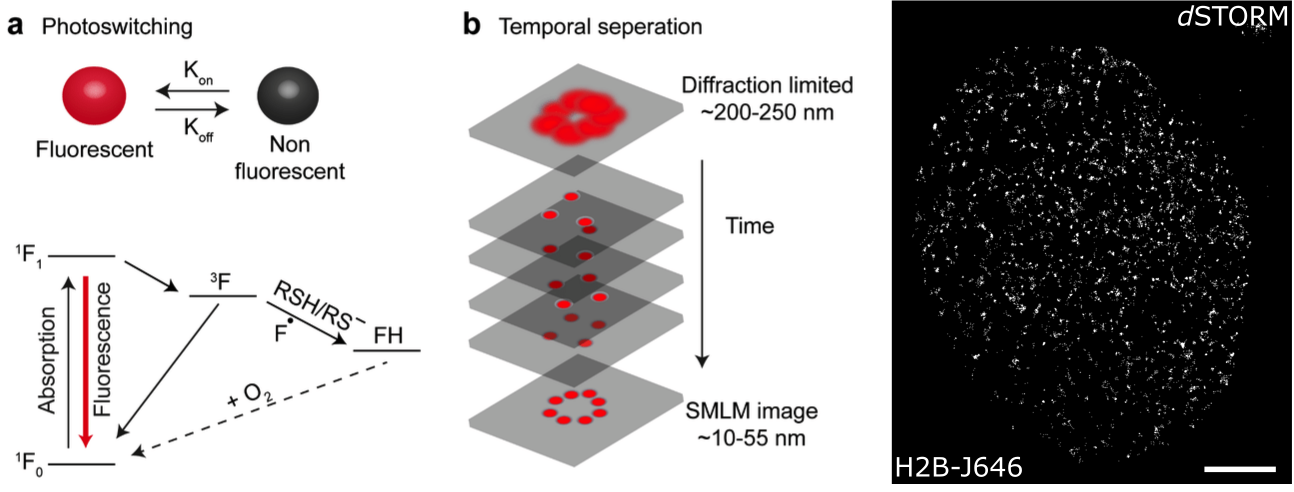
\includegraphics[width=\textwidth]{figures/Intro.png}
\caption{\textbf{Stochastic optical reconstruction microscopy (STORM)}. (A) Single molecules are resolved by separating their fluorescent emission in time, using fluorophores with multiple photophysical states (B) Example super-resolution image of H2B protein in a living Hela cell nucleus at 37C, 5 percent CO2. Image reconstructed from $10^{3}$ 10ms frames. Scalebar 5um.}
\end{figure}

Localization uncertainty, typically the RMSE of a maximum likelihood or similar statistical estimator, is bounded from below by the inverse of the Fisher information matrix, known as the Cramer-Rao lower bound (Chao 2016). Localization uncertainties in sparse conditions are often tens of nanometers, although recent work on integration of Bayesian priors with modulation enhanced SMLM (meSMLM) or structured illumination with MINFLUX, has reduced spatial resolution below to a few nanometers (Kalisvaart 2022, Gwosh 2020). Nevertheless, managing the increase in localization uncertainty at high labeling density remains a major bottleneck to SMLM. Static uncertainty due to molecular crowding can be partially amelioriated by using pairwise or higher-order temporal correlations within a pixel neighborhood, known as stochastic optical fluctuation imaging or SOFI (Dertinger 2009). Other approaches such as stimulated emission and depletion (STED) imaging bring control over the photophysical state of a chosen subset of the sample, yet the need for laser scanning prevents widespread application in live-cell studies. The spatial resolution and relative simplicity of SMLM techniques remains unmatched, inciting an effort to increase the resolution of SMLM techniques and explore avenues towards time resolved SMLM.

\subsection{Novel contributions to the field}

Here, we present single photon counting enhanced SMLM and a technique for super-resolution imaging of chromatin nanodomains in-vivo. We address dense SMLM by utilizing a high-speed single photon avalanche diode (SPAD) camera. SPAD cameras provide the necessary functionality for both single molecule localization and counting. Then, we present a more conventional dSTORM approach to study spatial organization of nucleosomes in living cells, with a particular focus on the structure of phase separated condensates containing bromodomain protein 4 (BRD4) protein.




%\ProvidesFile{ch-introduction.tex}[2022-10-05 ch-do-not-use-these-packages chapter]

\chapter{DO NOT USE THESE PACKAGES}

The
|\usepackage{|\Place{packagename}|}|
command is used to load a package.

Do not use these packages for the listed purposes.
Using them for these purposes is not compatible with \PurdueThesisLogo.\\

\noindent
\begin{tabularx}{\textwidth}{@{}lX@{}}
  \toprule
  \bf Name& \bf For\\
  \midrule
  babel&
    Translating ``Table of Contents'', etc\@. to foreign languages.
    Reported by Danushka Menikkumbura.
    Send email to {\tt latex@ecn.purdue.edu} if you need to
    typset multiple languages in your thesis.\\
  caption&
    Used to customize captions.
    Do not load this package, it is not compatible with \PurdueThesisLogo.\\
  subfig&
    For subfigures.
    This package is deprecated.
    Do not load this package.
    See page \pageref{pa:subfigures} for how to do subfigures.\\
  subfigure&
    For subfigures.
    This package is deprecated.
    Do not load this package.
    See page \pageref{pa:subfigures} for how to do subfigures.\\
  \bottomrule
\end{tabularx}


% Summary and/or conclusions are optional but often used.
% The summary and/or conclusions often are the last
% the last major division(s) of the text.
% Reference: TM2017 page 32.
%\ProvidesFile{ch-summary.tex}[2022-10-05 summary chapter]

\begin{VerbatimOut}{z.out}
\chapter{SUMMARY}

This is the summary chapter.


\section{First Section}

This is the first section of the summary chapter.
\end{VerbatimOut}

\MyIO


% Recommendations are optional.
% You may include recommendations as a major division if your
% subject matter and research dictate.
% Reference: TM2017 page 32.
%\ProvidesFile{ch-recommendations.tex}[2022-10-05 recommedations chapter]

\chapter{RECOMMENDATIONS}

Buy low.
Sell high.


% Test \begin{refsection}...\end{refsection}.
%\ProvidesFile{ch-test.tex}[2022-10-05 test chapter]

\begin{refsection}

\chapter{TEST ENVIRONMENTS AND PER-CHAPTER REFERENCES}

\verb+\cite[page v]{knuth2012}+ gives ``\cite[page v]{knuth2012}''.

\noindent
\verb+\cite[back cover]{lamport1994}+ gives ``\cite[back cover]{lamport1994}''.

\noindent
\verb+\cite{thesis2017}+ gives ``\cite{thesis2017}''.

\noindent
\verb+\cite{thesis2020}+ gives ``\cite{thesis2020}''.

This is an example of normal text.
This is an example of normal text.
This is an example of normal text.
This is an example of normal text.
This is an example of normal text.
This is an example of normal text.
This is an example of normal text.
This is an example of normal text.
This is an example of normal text.
This is an example of normal text.

\begin{definition}
  \ZZbaselinestretch{1.5}
  This is an example definition.
  This is an example definition.
  This is an example definition.
  This is an example definition.
  This is an example definition.
\end{definition}

This is an example of normal text.
This is an example of normal text.
This is an example of normal text.
This is an example of normal text.
This is an example of normal text.
This is an example of normal text.
This is an example of normal text.
This is an example of normal text.
This is an example of normal text.
This is an example of normal text.

\begin{observation}
  \ZZbaselinestretch{1.5}
  This is an example observation.
  This is an example observation.
  This is an example observation.
  This is an example observation.
  This is an example observation.
\end{observation}

This is an example of normal text.
This is an example of normal text.
This is an example of normal text.
This is an example of normal text.
This is an example of normal text.
This is an example of normal text.
This is an example of normal text.
This is an example of normal text.
This is an example of normal text.
This is an example of normal text.

\begin{proof}
  \ZZbaselinestretch{1.5}
  This is an example proof.
  This is an example proof.
  This is an example proof.
  This is an example proof.
  If \(a = b\) and \(b = c\) then \(a = c\).
\end{proof}

This is an example of normal text.
This is an example of normal text.
This is an example of normal text.
This is an example of normal text.
This is an example of normal text.
This is an example of normal text.
This is an example of normal text.
This is an example of normal text.
This is an example of normal text.
This is an example of normal text.

\begin{proposition}
  \ZZbaselinestretch{1.5}
  This is an example proposition.
  This is an example proposition.
  This is an example proposition.
  This is an example proposition.
  This is an example proposition.
\end{proposition}

This is an example of normal text.
This is an example of normal text.
This is an example of normal text.
This is an example of normal text.
This is an example of normal text.
This is an example of normal text.
This is an example of normal text.
This is an example of normal text.
This is an example of normal text.
This is an example of normal text.

\begin{theorem}
  \ZZbaselinestretch{1.5}
  This is an example theorem.
  This is an example theorem.
  This is an example theorem.
  This is an example theorem.
  This is an example theorem.
\end{theorem}

This is an example of normal text.
This is an example of normal text.
This is an example of normal text.
This is an example of normal text.
This is an example of normal text.
This is an example of normal text.
This is an example of normal text.
This is an example of normal text.
This is an example of normal text.
This is an example of normal text.

\begin{singlespace}
\def\sllnsez{[1] }
\PrintChapterBibliography
\end{singlespace}

\end{refsection}


% \immediate\setlength{\bibhang}{-3in}
% \immediate\setlength{\itemindent}{3in}
% \immediate\setlength{\rightmargin}{3in}

%
% This is only done if you are using BibLaTeX.
%
\makeatletter  % commented out on 2022-01-26
  \defbibenvironment{bibliography}
    {%
      \list
        {%
          \printtext[labelnumberwidth]%
          {%
            \printfield{prefixnumber}%
            \printfield{labelnumber}%
          }%
        }%
        {%
          \setlength{\bibhang}{1in} %%%%% was 0pt
          \setlength{\itemindent}{1in}%  -\leftmargin} %%%%% was 0pt
          \setlength{\itemsep}{\bibitemsep}%
          \setlength{\leftmargin}{0pt}%  .22in} % 0.42in}
          \setlength{\parsep}{\bibparsep}%
           \setlength{\rightmargin}{0.33in}%
        }%
    }
    {\endlist}
    {\item}
\makeatother  % commented out on 2022-01-26

% \immediate\setlength{\labelnumberwidth}{1.5in} %%%%% was commented out
\setlength{\labelwidth}{1.5in}
\def\sllnsez{[999] }

{%
  % Make _ in URLs visible.
  % \def\t{\char'137}%
  \catcode`*=\active
  \def*{\char'137}%  \char'137 is _
  \PrintBibliography
}

% Appendices are optional.  Not all theses contain appendices.
% An appendix is used for supplementary illustrative material,
% original data, computer programs, and other material that is not
% necessarily appropriate for inclusion within the text of your
% thesis.
% Reference: TM2017 page 33.
%
% Use ``\appendix'' for one appendix or ``\appendices'' for more than
% one appendix.
\appendices

% My filename conventions:
%     FILE THAT START WITH    ARE
%     ap-                     appendices
%     ch-                     chapters
%     gr-                     graphics
%     pa-                     packages
%     z                       temporary files

  % "About Appendices" appendix.
  %\ProvidesFile{ap-about-appendices.tex}[2022-10-05 about the appendicies appendix]

\begin{VerbatimOut}{z.out}
\chapter{ABOUT THE APPENDICES}

% Use single spacing in the appendices from now on to save space.
\ZZbaselinestretch{1}

\textcolor{red}{%
  \textbf{%
    These appendices are single-spaced to save space.
    Your thesis should use the default~1.5 line spacing.%
  }%
}

There are two groups of appendices.
The first group are general appendices;
the second group are domain-specific appendices.

These appendices are a series of examples.
They are a work in progress.

Each example consists of some \LaTeX\ output
followed by the corresponding input lines.
Some \LaTeX\ input lines only define things
and don't produce any output.
Each chunk in the input file begins with
\verb+\begin{VerbatimOut}{z.out}+
then has the \LaTeX\ input for the example,
% Don't literally end VerbatimOut on next line.
and ends with {\tt \char'134 end\char'173 VerbatimOut\char'175},
followed by a blank line,
followed by a line that begins with
|\My|.

\end{VerbatimOut}

\MyIO


\begin{VerbatimOut}{z.out}


\section{Paragraphs}

This is the first paragraph.
Paragraphs are separated by blank lines.

This is the second paragraph.


\section{Section Heading}

This is a sentence.
This is a sentence.
This is a sentence.
This is a sentence.
This is a sentence.


\subsection{Subsection heading}

This is a sentence.
This is a sentence.
This is a sentence.
This is a sentence.
This is a sentence.


\subsubsection{Subsubsection heading}

This is a sentence.
This is a sentence.
This is a sentence.
This is a sentence.
This is a sentence.
\end{VerbatimOut}

\MyIO



\begin{VerbatimOut}{z.out}


\section{Text math}

If items in a list are narrow like these Greek characters,\\
    \I2 \verb+$\alpha$, $\beta$, and $\gamma$+\\
I'd input the line like this\\
    \I2 \verb+$\alpha$,~$\beta$, and~$\gamma$+\\
where the \verb+~+ is a tie
that ties together what's before and after it on the same line of the output
\cite[page~92]{knuth2012}.

This text is the correct length to show what happens with and without ties:
$\alpha$,
$\beta$,
and $\gamma$.
See how the line gets split
and the~$\gamma$ is at the beginning of the line?

This text is the correct length to show what happens with and without ties:
$\alpha$,~$\beta$,
and~$\gamma$.
See how the line gets compressed a little bit so the~$\gamma$
is not at the beginning of the line?
\end{VerbatimOut}

\MyIO


  % "Bugs" appendix.
  %\ProvidesFile{ap-bugs}[2022-10-14 bugs appendix]

\makeatletter
\newcommand{\bug}[2]
  {%
    \vspace{6pt}
    \noindent
    {%
      \bfseries
      \ifthen{\equal{high}{#2}}{\color{red}}%
      \ifthen{\equal{low}{#2}}{\color{green}}%
      \ifthen{\equal{done}{#2}}{\color{black}}%
      \ifthen{\equal{fixed}{#2}}{\color{black}}%
      \ifthen{\equal{wait}{#2}}{\color{black}}%
      \ifthen{\equal{not}{#2}}{\color{gray}}%
      {\fontsize{9}{10}\reset@font\bf BUG}
      #1.
    }%
    \ignorespaces
  }
\makeatother

\chapter{BUGS}

This appendix lists all bugs/comments/issues/etc\@.
under the generic name `bug'.
Each bug is assigned a number when I learn of it.
Bug numbers are 1, 2,~\ldots~.
I started keeping track of bugs in this fashion on February 26, 2022,
and some previously known bugs are included in this list.
A color indicates a bug's priority:

\begin{tabular}{@{}ll@{}}
  \toprule
  \bf Description& \bf Color\\
  \midrule
  done or waiting on someone else& \color{black}black\\
  high priority or easy to do& \color{red}red\\
  low priority& \color{green}green\\
  not prioritized yet& \color{gray}gray\\
  \bottomrule\\
\end{tabular}

See the ap-bugs.tex file for the \LaTeXLogo\ input for this appendix.


\section{These bugs need to be looked at}

% I need to fix the following things in \PurdueThesis.
% They are listed in bug number order.

\bug{1}{high}
Table of Contents is double-spaced instead of 1\sfrac12 spacing.
{\small
  Tighten up section and less significant headings spacing?
  Reported by Anita Adams Sale on 2021-03-17.%
}

\bug{2}{high}
List of Figures indented $\approx$\sfrac14 inch
more than List of Tables.
{\small
  Reported by Anita Adams Sale on 2021-03-17.
  Still happening on 2021-11-30.
  Looked ok on 2022-08-26
  but I think this problem is probably intermittent.
  Keep Ashlee Messersmith,
  Anita Adams Sale,
  and Sherrie Tucker informed.%
}

\bug{6}{not}
APA reference style indents references too far on left.
{\small
Reported by Mark Senn on 2021-04-08.%
}

\bug{8}{not}
Use ``Last Accessed: yyyy-mm-dd.'' urldate in bibliography.
{\small
  Reported by Mark Senn on 2021-04-19.%
}

\bug{9}{low}
Check that |@{}| is before the left column
and after the right column in all tables.
{\small
  Reported by Mark Senn on 2021-04-19.%
}

\bug{11}{low}
Bibliography change:
Change,
for example,
``Acoustical Science and Technology, vol.~23, no.~1''
to
``Acoustical Science and Technology {\bfseries 23\/} ({\bfseries 1\/})''.
{\small
  Reported by Daniel Joesph Carr on 2021-06-16.%
}

\bug{12}{low}
Bibliography change:
Change,
for example,
|M.~Abramowitz and I.A.~Stegun, Eds.,|
to
|M.~Abramowitz and I.A.~Stegun, editors,|.
{\small
  Reported by Daniel Joesph Carr on 2021-06-16.
}

\bug{13}{low}
Headings containing a SmallCaps font do not work.
{\small
  Reported by Javad (Nima) Darivandpour on 2021-06-29.
  See \ref{section-headings-with-smallcaps-font}.%
}

\bug{14}{low}
On Overleaf only,
when using
|\def\ZZshowtimestamp{true}|,
the time and sometimes the date
are wrong at the top of the page.
{\small
  Reported by Mark Senn on 2022-02-25.
  This might be due to using
  |\ExplSyntaxOn| \ldots |\ExplSyntaxOff|
  and having |:| and/or other characters having the wrong catcode.
}

\bug{15}{not}
Left reference section margin is ok if a person has 10--99 references.
{\small
  Figure out how to adjusting margin for 1--9 or over 99 references.
  Reported by Mark Senn on unknown date.
}

\bug{19}{high}
|Bibliography| and |References| missing from navigation panel.
{\small
  Reported by Mark Senn on 2022-02-28.
  REFERENCES was in navigation panel on 2022-08-26.
}

\bug{20}{high}
|Bibliography| and |References| should be in all caps.
{\small
  Reported by Mark Senn on 2022-02-28.
  REFERENCES was in all caps on 2022-08-26.%
}

\bug{21}{low}
IE students should be able
to specify IEEE
or APA bibliography format.
{\small
  Reported by Patrick Brunese on 2022-03-04.%
}

\section{These bugs are waiting on a reply from someone other than Mark Senn}

\bug{10}{wait}
Using
|linktoc = section|
does not work with captions with
|\frac|.
{\small
  Reported by Mark Senn on 2021-05-27.
  In the short-term,
  check with Ashlee Messersmith
  if {\tt linktoc = page} can be used.
  If that's ok make the change
  and look into changing captions from my code
  to \LaTeXLogo's code.
  Waiting on Ashlee Messersmith.
}

\section{These bugs have been rejected or fixed}

\bug{3}{done}
Use ``Last Accessed: dd/mm/yy.'' urldate in bibliography.
{\small
  Reported by Priyank Kalgaonkar on 2021-04-06.
  Answered by Mark Senn on 2022-02-27.
  The United States uses mm/dd/yy and other countries use dd/mm/yy
  \cite{cms17-ambiguous-dates}.
  I recommend using what your bibliography style defines
  or the unambiguous ISO 8601 standard yyyy-mm-dd
  \cite{cms17-iso-dates}.%
}

\bug{4}{done}
Change citation, e.g., |[6], [71]| to |[6,71]|.
{\small
  Reported by Mark Senn on 2021-04-07.
  Fixed on 2022-04-14.
  Tested ok on 2022-04-14.%
}

\bug{5}{done}
Change citation, e.g., |[6], [7], [8]| to |[6-8]|.
{\small
  Reported by Mark Senn on 2021-04-07.
  Fixed on 2022-04-14.
  Tested ok on 2022-04-14.%
}

\bug{7}{fixed}
Non-nested description environments have bold items.
Nested description environments have non-bold items.
How come?
Are the indentations correct?
{\small
  Reported by Mark Senn on 2021-04-09.
  Tested ok on 2021-05-31.%
}

\bug{16}{fixed}
Add DTECH degree.
{\small
  Reported by Mark Senn on unknown date.
  Program ``Technology''
  and degree ``Doctor of Technology'' worked ok
  on 2022-08-26.%
}

\bug{17}{fixed}
Allow |,| (comma) in |\title|.
{\small
  Reported by Mark Senn on unknown date.
  Tested ok on 2021-11-30.%
}

\bug{18}{fixed}
Allow |\\| in |\title|.
{\small
  Reported by Mark Senn on unknown date.
  Tested ok on 2021-11-30.%
}


  % Check margins.
  %\ProvidesFile{ap-check-margins.tex}[2022-10-05 check margins appendix]

\begin{VerbatimOut}{z.out}
\chapter{CHECK MARGINS}
\end{VerbatimOut}

\MyIO


\begin{VerbatimOut}{z.out}
\MyRepeat{This is a sentence. }{300}
\end{VerbatimOut}

\MyIO


  % Demonstrate how to do separate appendices per chapter.
  %\ProvidesFile{ap-chapter-appendices.tex}[2022-10-05 chapter appendices appendix]

\begin{VerbatimOut}{z.out}
\chapter{CHAPTER APPENDICES}

Using |\chapterappendix|
or |\chapterappendices|
in a chapter will number sections,
for example,
1.1,
1.2,
\ldots,
1.A,
1.B,
\ldots\,.

Using |\chapterappendix|
or |\chapterappendices|
in an appendix will number sections,
for example,
A.1,
A.2,
\ldots,
A.A,
A.B,
\ldots\,.

I suggest only using |\chapterappendix|
or |\chapterappendices| in chapters---%
using them in appendices is too confusing.
\end{VerbatimOut}

\MyIO


\begin{VerbatimOut}{z.out}
\newpage


\section{This is a section heading}

This is a paragraph.

Use \verb+\chapterappendix+ or \verb+\chapterappendices+
to make sections until the end of the next chapter
be appendices.


\chapterappendix


\section{This is a chapter appendix}

This is a paragraph.
\end{VerbatimOut}

\MyIO


  % Demonstrate how to do separate references per chapter.
  % \ProvidesFile{ap-chapter-references.tex}[2022-10-05 chapter references appendix]

\begin{VerbatimOut}{z.out}
\begin{refsection}
\chapter{CHAPTER REFERENCES}

This is a paragraph.

\section{This is a section heading}

This is a paragraph.

|\cite{reid2013}| gives \cite{reid2013}.
|\cite{test-long-title}| gives \cite{test-long-title}.
|\cite{sexon2012}| gives \cite{sexon2012}.
|\cite{test-long-titleb}| gives \cite{test-long-titleb}.

\PrintChapterBibliography
\end{refsection}
\end{VerbatimOut}

\MyIO


  % Citations and references.
  \ProvidesFile{ap-citations-references.tex}[2022-10-05 citations and references appendix]

\begin{VerbatimOut}{z.out}
\chapter{CITATIONS AND REFERENCES}
\end{VerbatimOut}

\MyIO


\begin{VerbatimOut}{z.out}

This chapter contains information about citations
and references---how to cite a reference in the text
and the fine points of defining a bibliography
(also called ``References'')
entry.
\end{VerbatimOut}

\MyIO


\begin{VerbatimOut}{z.out}


\section{Citations}
\end{VerbatimOut}

\MyIO


\begin{VerbatimOut}{z.out}
For \LaTeX\ answers I refer to
\cite{lamport1994}
and then to
\cite{goossens1994}
or
\cite{kopka1999}.
\cite{kopka1999}
is an update to
\cite{kopka1995}.
\end{VerbatimOut}

\MyIO


\begin{VerbatimOut}{z.out}

Here is an example .bib file entry:

{\footnotesize
\begin{verbatim}
@misc{example2020,
  address   = {Imaginaryville, Indiana},
  author    = {Andrew Anteater and Bertha Bear and Charles Cheetah and Davida Deer
                and Ethan Eagle},
  date      = {2020-10-27},
  doi       = {00.0000/000-0-000-00000-0},
  editor    = {Mark Senn},
  edition   = {2},
  isbn      = {{000\FigureDash 0\FigureDash 000\FigureDash 00000\FigureDash 0}},
  publisher = {Bogus International Publishing Company},
  title     = {An Imaginary Document Not About {Mark Senn} or {NASA}},
  url       = {https://bogus.com/bogus.html},
  urldate   = {2020-10-27},
  version   = {1.0},
}
\end{verbatim}
}
\end{VerbatimOut}

\MyIO


\begin{VerbatimOut}{z.out}
\PurdueThesisLogo\ only uses \BibLaTeXLogo.
Here are some example \BibLaTeXLogo\ citations for your document.

\begin{tabular}{@{}ll@{}}
  \bf Input&                        \bf Output\\
  \verb+\cite{example2020}+&        \cite{example2020}\\
  \verb+\cite*{example2020}+&       \cite*{example2020}\\
  \verb+\citeauthor{example2020}+&  \citeauthor{example2020}\\
  \verb+\citeauthor*{example2020}+& \citeauthor*{example2020}\\
  \verb+\citedate{example2020}+&    \citedate{example2020}\\
  \verb+\citetitle{example2020}+&   \citetitle{example2020}\\
  \verb+\citetitle*{example2020}+&  \citetitle*{example2020}\\
  \verb+\citeurl{example2020}+&     \citeurl{example2020}\\
  \verb+\citeyear{example2020}+&    \citeyear{example2020}\\
  \verb+\parencite{example2020}+&   \parencite{example2020}\\
  \verb+\textcite{example2020}+&    \textcite{example2020}\\
\end{tabular}
\end{VerbatimOut}

\MyIO


\begin{VerbatimOut}{z.out}


\section{References}
\end{VerbatimOut}

\MyIO


\begin{VerbatimOut}{z.out}

Emily Spreen wrote that the following URLs are invisible in the PDF file.
They worked fine for me on 2021-04-08.
See \cite{hambleton}, \cite{gerstenmaier}, and \cite{gerstenmaier2} in the REFERENCES.

{\footnotesize
\begin{verbatim}
@misc{hambleton,
  key = {Deep Space Gateway},
  title = {{Deep Space Gateway to Open Opportunities for Distant Destinations}},
  note = {Editor: Kathryn Hambleton},
  year = {2018},
  month = {August 24,},
  howpublished = {\url{https://www.nasa.gov/feature/deep-space-gateway-to-open-...}},
  organization = {NASA},
}
\end{verbatim}
}

{\footnotesize
\begin{verbatim}
@misc{gerstenmaier,
  author = {William H. Gerstenmaier},
  title = {{Progress in Defining the Deep Space Gateway and Transport Plan}},
  month = {March},
  year = {2017},
  howpublished = {\url{https://www.nasa.gov/sites/default/files/atoms/files/...}},
  organization = {NASA},
}
\end{verbatim}
}

I suggest using the following
(added a `2' to the key so they'd have separate entries in the references.).
{\footnotesize
\begin{verbatim}
@misc{gerstenmaier2,
  author = {William H. Gerstenmaier},
  date = {2017-03},
  title = {{Progress in Defining the Deep Space Gateway and Transport Plan}},
  url = {https://www.nasa.gov/sites/default/files/atoms/files/nss_chart_v23.pdf},
  organization = {NASA},
}
\end{verbatim}
}
\end{VerbatimOut}


\MyIO


  % Common mistakes.
  %\ProvidesFile{ap-common-mistakes.tex}[2022-10-05 common mistakes appendix]

\begin{VerbatimOut}{z.out}
\chapter{COMMON MISTAKES}

The following Headings, Mathematics, and Text
sections describe some common mistakes.


\section{Headings}

\textcite[page~289]{farkas2011}
wrote

\begin{quotation}
  The practice of stacking headings
  is routinely condemned by style manuals
  and other authorities.
  Here is a typical statement,
  taken from Houghton Mifflin's guidelines for authors.
  \begin{quotation}
    Avoid ``stacking'' heads,
    or placing two levels
    of headings together without intervening text.
    A heading cannot substitute
    for the transitional
    or introductory paragraphs
    that guide the reader through a chapter.
    Remember too that a chapter opening looks better in type
    when one
    or more paragraphs
    of text precede the first heading.
  \end{quotation}
\end{quotation}
\end{VerbatimOut}

\MyIO


\begin{VerbatimOut}{z.out}


\section{Mathematics}

\subsection{Put a little extra horizontal space before dx}
\end{VerbatimOut}
\MyIO


\begin{VerbatimOut}{z.out}


\section{Text}
\end{VerbatimOut}

\MyIO


\begin{VerbatimOut}{z.out}

\subsection{e.g.,}
\ix{e.g.}

``e.g.'' should always be followed by a comma.
\end{VerbatimOut}

\MyIO


\begin{VerbatimOut}{z.out}

\subsection{``et al.'' is an abbreviation}
\ix{et al.}

The phrase ``et al.''
is an abbreviation
and should always be followed by a period.
It should be in the normal font for your document---%
do not italicize or underline it.

Example:\\[6pt]
\indent\indent
\begin{tabular}{@{}ll@{}}
  input&   \verb+Thun et al.~used data from Santa Claus.+\\
  output&  Thun et al.~used data from Santa Claus.\\
  comment& my recommendation\\[6pt]
  input&   \verb+Thun et al. used data from Santa Claus.+\\
  output&  Thun et al. used data from Santa Claus.\\
  comment& too much space after period---\LaTeX\ thinks period is end of sentence\\[6pt]
  input&   \verb+Thun et al\@. used data from Santa Claus.+\\
  output&  Thun et al\@. used data from Santa Claus.\\
  comment& spacing is right but the ``et al.'' could occur at end of a line\\
\end{tabular}
\end{VerbatimOut}

\MyIO


\begin{VerbatimOut}{z.out}

\subsection{i.e.,}
\ix{i.e.}

``i.e.'' should always be followed by a comma.
\end{VerbatimOut}

\MyIO


  % Defining commands.
  %\ProvidesFile{ap-defining-commands.tex}[2022-10-05 defining commands appendix]

\begin{VerbatimOut}{z.out}
\chapter{DEFINING COMMANDS}

The next paragraph demonstrates how to define and use a command.

\renewcommand{\t}[2]
{% The "{%" hides the space caused by the newline.  LaTeX ignores leading spaces on a line.
  Editors recommend that a #1 should never be
  followed by a #2 without some intervening text.
}

\t{chapter title}{section heading}
I suggest writing for readers.
Break the rules if necessary.
\end{VerbatimOut}

\MyIO


  % Figures.
  %\ProvidesFile{ap-figures.tex}[2022-10-05 figures appendix]

\begin{VerbatimOut}{z.out}
\chapter{FIGURES}
\end{VerbatimOut}

\MyIO


\begin{VerbatimOut}{z.out}

The
\verb+h+
specifier used in all the examples below
tells \LaTeX\ to put the figure
``here''
instead of trying
to find a good spot
at the top or bottom of a page.
Specifiers can be combined,
for example,
``\verb+\begin{figure}[htbp!]+''.
\end{VerbatimOut}

\MyIO


\begin{VerbatimOut}{z.out}

The complete list of figure placement specifiers:
\vspace*{6pt}
\begin{center}
  \begin{tabular}{@{}ll@{}}
    \toprule
    \bf Specifier& \bf Description\\
    \midrule
    \noalign{\vspace*{2pt}}
    \tt b& bottom of page\\
    \tt h& here on page\\
    \tt p& on separate page of figures\\
    \tt t& top of page\\
    \tt !& try hard to put figure as early as possible\\
    \bottomrule
  \end{tabular}
\end{center}
\index{figure!placement specifiers (\verb+b+, \verb+h+, \verb+p+, \verb+t+, {\tt \char'041})}
\index{\verb+\begin{tabular}+}
\end{VerbatimOut}

\MyIO


% !!!! Label ``fi:not-centered'' is ``\ref{fi:not-centered}''.
% !!!! Label ``sf:four-parts-c'' is ``\ref{sf:four-parts-c}''.

\begin{VerbatimOut}{z.out}

% MyRepeat is defined in MyRepeat.sty.
\MyRepeat{This is the first paragraph.  }{5}
\end{VerbatimOut}

\MyIO


\begin{VerbatimOut}{z.out}

\begin{figure}
  This is the figure.
  \caption{%
    Allocation to Common Edge for
    \(p(x_i) = 1-e^{-x_iz}\)% \frac{-x_i}z}\)%
  }
\end{figure}
\end{VerbatimOut}

\MyIO



\begin{VerbatimOut}{z.out}

\begin{figure}[ht]
  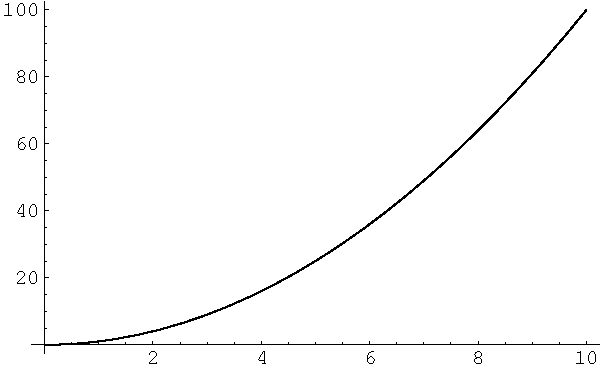
\includegraphics{gr-plot.pdf}
  \caption
  {%
    By default figures are not centered.
    This is a long caption to demonstrate that captions are single spaced.
    This is a long caption to demonstrate that captions are single spaced.%
  }
  \label{fi:not-centered}
\end{figure}
\end{VerbatimOut}

\MyIO


\begin{VerbatimOut}{z.out}

\MyRepeat{This is the second paragraph.  }{10}
\end{VerbatimOut}

\MyIO


\begin{VerbatimOut}{z.out}

\begin{figure}[ht]
  \centering
  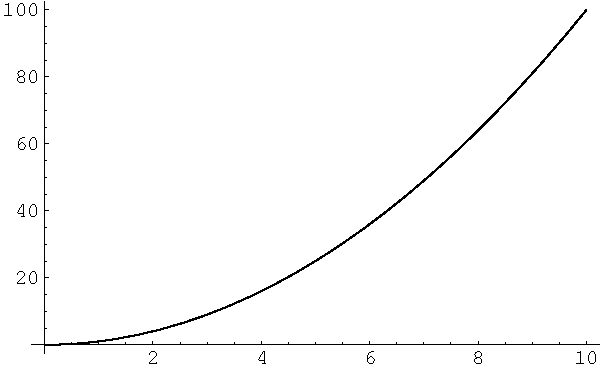
\includegraphics{gr-plot.pdf}
  \caption{Use {\tt \char'134centering\/} to center figures.}
  \label{fi:centered}
\end{figure}
\end{VerbatimOut}

\MyIO


\begin{VerbatimOut}{z.out}

\MyRepeat{This is the third paragraph.  }{15}
\end{VerbatimOut}

\MyIO


\begin{VerbatimOut}{z.out}

\begin{figure}[ht]
  \centering
  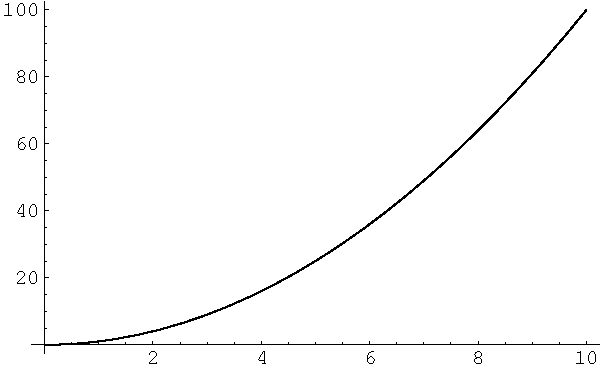
\includegraphics{gr-plot.pdf}
  \caption{This is another figuure.}
  \label{fi:another}
\end{figure}
\end{VerbatimOut}

\MyIO


\begin{VerbatimOut}{z.out}

\MyRepeat{This is the fourth paragraph.  }{10}
\end{VerbatimOut}

\MyIO


\begin{VerbatimOut}{z.out}
  
% See pages 4--5 of
%   http://mirrors.ibiblio.org/CTAN/macros/latex/contrib/caption/subcaption.pdf
% for how to use \subcaptionbox.
\begin{figure}[ht]
  % Center the entire figure (containing the two subfigures).
  \centering 
    % The \subcaptionbox for the first subfigure.
    \subcaptionbox
      % The first subcaption with a \label.
      % Use \ref{sf:two-parts-a} to print the subcaption number.
      {First subcaption.\label{sf:two-parts-a}}%
      % The first subfigure is this wide.
      [2in]%
      % This is the first subfigure.
      % You'll usually use an \includegraphics{filename}
      % inside the braces on the next line.
      {\bfseries First subfigure.}%
    % Put 0.5 inches of blank space between the subfigures.
    \hskip 0.5truein
    \subcaptionbox
      {Second subcaption.\label{sf:two-parts-b}}%
      [2in]%
      {\bfseries Second subfigure.}%
    % The caption for the entire figure (containing two subfigures).
    \caption{This figure has two subfigures arranged horizontally.}
    % The label for the entire figure.
    \label{fi:two-horizontal-parts}
\end{figure}
\ix{figure!subfigures!\(\text{1 row} \times \text{2 columns}\)}
\end{VerbatimOut}

\label{pa:subfigures}

\MyIO


\begin{VerbatimOut}{z.out}

\MyRepeat{This is the fifth paragraph.  }{10}
\end{VerbatimOut}

\MyIO


\begin{VerbatimOut}{z.out}

% See pages 4--5 of
%   http://mirrors.ibiblio.org/CTAN/macros/latex/contrib/caption/subcaption.pdf
% for how to use \subcaptionbox.
\begin{figure}[ht]
  % Center the entire figure (containing the two subfigures).
  \centering
    % The \subcaptionbox for the first subfigure.
    \vbox{\subcaptionbox  % use \vbox to stack subcaption boxes vertically
      % The first subcaption with a \label.
      % Use \ref{sf:two-vertical-parts-a} to print the subcaption number.
      {First subcaption.\label{sf:two-vertical-parts-a}}
      [2in]%
      {\bfseries First subfigure.}}%
    % Put \baselineskip blank space between the subfigures.
    \vspace*{\baselineskip}
    % The \subcaptionbox for the second subfigure.
    \vbox{\subcaptionbox  % use \vbox to stack subcaption boxes vertically
      {Second subcaption.\label{sf:two-vertical-parts-b}}
      [2in]%
      {\bfseries Second subfigure.}}%
  \caption{This figure has two subfigures arranged vertically.}
  \label{fi:two-vertical-parts}
\end{figure}
\ix{figure!subfigures!\(\text{2 rows} \times \text{1 column}\)}
\end{VerbatimOut}

\MyIO


\begin{VerbatimOut}{z.out}

\MyRepeat{This is the sixth paragraph.  }{10}
\end{VerbatimOut}

\MyIO


\begin{VerbatimOut}{z.out}
  
% See pages 4--5 of
%   http://mirrors.ibiblio.org/CTAN/macros/latex/contrib/caption/subcaption.pdf
% for how to use \subcaptionbox.
\begin{figure}[ht]
  \centering
    \subcaptionbox
      {First subcaption.\label{sf:four-parts-a}}
      [2in]%
      {\bfseries First subfigure.}%
    \hskip 0.5truein
    \subcaptionbox
      {Second subcaption.\label{sf:four-parts-b}}
      [2in]%
      {\bfseries Second subfigure.}%
    \vspace*{\baselineskip}
    \subcaptionbox
      {Third subcaption.\label{sf:four-parts-c}}
      [2in]%
      {\bfseries Third subfigure.}%
    \hskip 0.5truein
    \subcaptionbox
      {Fourth subcaption.\label{sf:four-parts-d}}
      [2in]%
      {\bfseries Fourth subfigure.}%
  \caption{This figure has four parts.}
  \label{fi:four-parts}
\end{figure}
\ix{figure!subfigures!\(\text{2 rows} \times \text{2 columns}\)}
\end{VerbatimOut}

\MyIO


\begin{VerbatimOut}{z.out}

\MyRepeat{This is the seventh paragraph.  }{10}
\end{VerbatimOut}

\MyIO


\begin{VerbatimOut}{z.out}

\newpage

\begin{figure}[ht]
  \centering 
    % Use a 5" font.
    {\fontsize{5in}{5in}\selectfont\(\hspace*{-0.07em}\sqrt 2\)}
    \caption{%
      A big ``\(\sqrt 2\)''.
      \LaTeX\ can make output big enough for T-shirts or posters.
      Square roots are printed with space before them,
      I put some negative horizontal space before this one to center it.%
    }
\end{figure}
\ix{figure!\(\sqrt 2\)}
\end{VerbatimOut}

\MyIO

\UndefineShortVerb{\|}  % so "|" in not a special character
\ix{subfigure|see{figure, subfigures}}
\DefineShortVerb{\|}  % so "|verbatim|" will be verbatim


\begin{figure}
  This is the figure.
  \caption{%
    Allocation to Common Edge for
    \(p(x_i) = 1-e^{-x_iz}\)% \frac{-x_i}z}\)%
  }
\end{figure}

\begin{VerbatimOut}{z.out}

\newpage

The remainder of this file tests having lots of figures.
There are 20 figures in this test.

\begin{figure}[ht]
  \centering
  
\includegraphics[scale=0.5]{gr-metapost-tally-01.pdf}
  \caption{Test figure 1 of 20.}
  \label{fi:1of20}
\end{figure}

\begin{figure}[ht]
  \centering
  
\includegraphics[scale=0.5]{gr-metapost-tally-02.pdf}
  \caption{Test figure 2 of 20.}
  \label{fi:2of20}
\end{figure}

\begin{figure}[ht]
  \centering
  
\includegraphics[scale=0.5]{gr-metapost-tally-03.pdf}
  \caption{Test figure 3 of 20.}
  \label{fi:3of20}
\end{figure}

\begin{figure}[ht]
  \centering
  
\includegraphics[scale=0.5]{gr-metapost-tally-04.pdf}
  \caption{Test figure 4 of 20.}
  \label{fi:4of20}
\end{figure}

\begin{figure}[ht]
  \centering
  
\includegraphics[scale=0.5]{gr-metapost-tally-05.pdf}
  \caption{Test figure 5 of 20.}
  \label{fi:5of20}
\end{figure}

\begin{figure}[ht]
  \centering
  
\includegraphics[scale=0.5]{gr-metapost-tally-06.pdf}
  \caption{Test figure 6 of 20.}
  \label{fi:6of20}
\end{figure}

\begin{figure}[ht]
  \centering
  
\includegraphics[scale=0.5]{gr-metapost-tally-07.pdf}
  \caption{Test figure 7 of 20.}
  \label{fi:7of20centered7}
\end{figure}

\begin{figure}[ht]
  \centering
  
\includegraphics[scale=0.5]{gr-metapost-tally-08.pdf}
  \caption{Test figure 8 of 20.}
  \label{fi:8of20}
\end{figure}

\begin{figure}[ht]
  \centering
  
\includegraphics[scale=0.5]{gr-metapost-tally-09.pdf}
  \caption{Test figure 9 of 20.}
  \label{fi:9of20}
\end{figure}

\begin{figure}[ht]
  \centering
  
\includegraphics[scale=0.5]{gr-metapost-tally-10.pdf}
  \caption{Test figure 10 of 20.}
  \label{fi:10of20}
\end{figure}

\begin{figure}[ht]
  \centering
  
\includegraphics[scale=0.5]{gr-metapost-tally-11.pdf}
  \caption{Test figure 11 of 20.}
  \label{fi:11of20}
\end{figure}

\begin{figure}[ht]
  \centering
  
\includegraphics[scale=0.5]{gr-metapost-tally-12.pdf}
  \caption{Test figure 12 of 20.}
  \label{fi:12of20}
\end{figure}

\begin{figure}[ht]
  \centering
  
\includegraphics[scale=0.5]{gr-metapost-tally-13.pdf}
  \caption{Test figure 13 of 20.}
  \label{fi:13of20}
\end{figure}

\begin{figure}[ht]
  \centering
  
\includegraphics[scale=0.5]{gr-metapost-tally-14.pdf}
  \caption{Test figure 14 of 20.}
  \label{fi:14of20}
\end{figure}

\begin{figure}[ht]
  \centering
  
\includegraphics[scale=0.5]{gr-metapost-tally-15.pdf}
  \caption{Test figure 15 of 20.}
  \label{fi:15of20}
\end{figure}

\begin{figure}[ht]
  \centering
  
\includegraphics[scale=0.5]{gr-metapost-tally-16.pdf}
  \caption{Test figure 16 of 20.}
  \label{fi:16of20}
\end{figure}

\begin{figure}[ht]
  \centering
  
\includegraphics[scale=0.5]{gr-metapost-tally-17.pdf}
  \caption{Test figure 17 of 20.}
  \label{fi:17of20}
\end{figure}

\begin{figure}[ht]
  \centering
  
\includegraphics[scale=0.5]{gr-metapost-tally-18.pdf}
  \caption{Test figure 18 of 20.}
  \label{fi:18of20}
\end{figure}

\begin{figure}[ht]
  \centering
  
\includegraphics[scale=0.5]{gr-metapost-tally-19.pdf}
  \caption{Test figure 19 of 20.}
  \label{fi:19of20}
\end{figure}

\begin{figure}[ht]
  \centering
  
\includegraphics[scale=0.5]{gr-metapost-tally-20.pdf}
  \caption{Test figure 20 of 20.}
  \label{fi:20of20}
\end{figure}
\end{VerbatimOut}

\MyIO


  % Frequently Asked Questions.
  %\ProvidesFile{ap-frequently-asked-questions}[2022-10-05 frequently asked questions appendix]

\newcommand{\MyA}{\textbf{A: }}

\makeatletter
\newcommand{\faq}[2]
  {%
    \vspace{6pt}
    \noindent
    {%
      \bfseries
      \ifthen{\equal{high}{#2}}{\color{red}}%
      \ifthen{\equal{medium}{#2}}{\color{yellow}}%
      \ifthen{\equal{low}{#2}}{\color{green}}%
      \ifthen{\equal{done}{#2}}{\color{black}}%
      \ifthen{\equal{fixed}{#2}}{\color{black}}%
      \ifthen{\equal{wait}{#2}}{\color{black}}%
      \ifthen{\equal{not}{#2}}{\color{gray}}%
      {\fontsize{9}{10}\reset@font\bf FAQ}
      #1.
    }%
    \ignorespaces
  }
\makeatother
  
\chapter{FREQUENTLY ASKED QUESTIONS}

This appendix lists all frequently asked questions.
Each frequently asked question is assigned a number when I learn of it.
Numbers are 1, 2,~\ldots~.
I started keeping track
of frequently asked questions
in this fashion
on March 1, 2022.

\begin{tabular}{@{}ll@{}}
  \toprule
  \bf Priority& \bf Color\\
  \midrule
  high or easy& \color{red}red\\
  medium& \color{yellow}yellow\\
  low& \color{green}green\\
  waiting on someone else& \color{black}black\\
  done& \color{black}black\\
  not assigned yet& \color{gray}gray\\
  \bottomrule\\
\end{tabular}

See the
|ap-frequently-asked-questions.tex|
file
for the \LaTeXLogo\ input
for this appendix.


\section{These questions need to be answered}


\section{These questions are waiting on a reply from someone other than Mark Senn}


\section{These questions have been answered}

The subsection headings below are what part of the document
the question is about.


\subsection*{Everywhere}
\faq{1}{done}
The \LaTeXLogo\ input\\
% \I2 \verb+$a | b$+\qquad
(Mark Senn recommends using \verb+\(a | b\)+ instead)\\
%   {\tt\char'134(\$a \char'174\ \$b\char'134)}
%   instead%
% )\\
gives\\
\I2 |! LaTeX Error: Command \ttfamily invalid in math mode.|\\
Reported by Negin Karisani.\\
\MyA
In thesis.tex, change\\
\I2 \verb+\DefineShortVerb{\|} % so "|verbatim|" will be verbatim+\\
% {\tt
%   \char'134 DefineShortVerb%
%   \{\char'134\char'174\}\ \ %
%   \% so "\char'174 verbatim\char'174" will be verbatim%
% }\\
to\\
\I2 \verb+% \DefineShortVerb{\|} % so "|verbatim|" will be verbatim+
% {\tt
%   \%\ \char'134 DefineShortVerb%
%   \{\char'134\char'174\}\ \ %
%   \% so "\char'174 verbatim\char'174" will be verbatim%
% }


\subsection*{Table of Contents}

\faq{2}{done}
I want text instead of page number to be the link
in the table of contents.
Asked by Danushka Menikkumbura on 2022-03-11.\\
\MyA
In PurdueThesis.cls change \verb+linktoc = page+
to \verb+linktoc = section+.
I do not recommend doing this because
\begin{itemize}
  \item
    you'll need to put this change
    in new PurdueThesis.cls files in the future
  \item
    people are used to using page numbers instead
    of chapter/section/etc. titles for where they
    start
\end{itemize}


  % Graphics.
  %\ProvidesFile{ap-graphics.tex}[2022-10-05 graphics appendix]

\begin{VerbatimOut}{z.out}
\chapter{GRAPHICS}

There are many ways to make graphics for \LaTeX.
I like to use a system that uses \LaTeX\ fonts
so the appearance of the output is professional.
\end{VerbatimOut}

\MyIO


\begin{VerbatimOut}{z.out}

\section{MATLAB programming language}
\ix{MATLAB programming language}

\def\gray#1{\colorbox{gray!15}{#1}}
\def\lightred#1{\colorbox{red!15}{#1}}
\def\lightgreen#1{\colorbox{green!20}{#1}}
\lightgreen{%
  By default,
  MATLAB supports a subset of TeX markup
  \cite{mathworks-help-center-text-properties}.
}

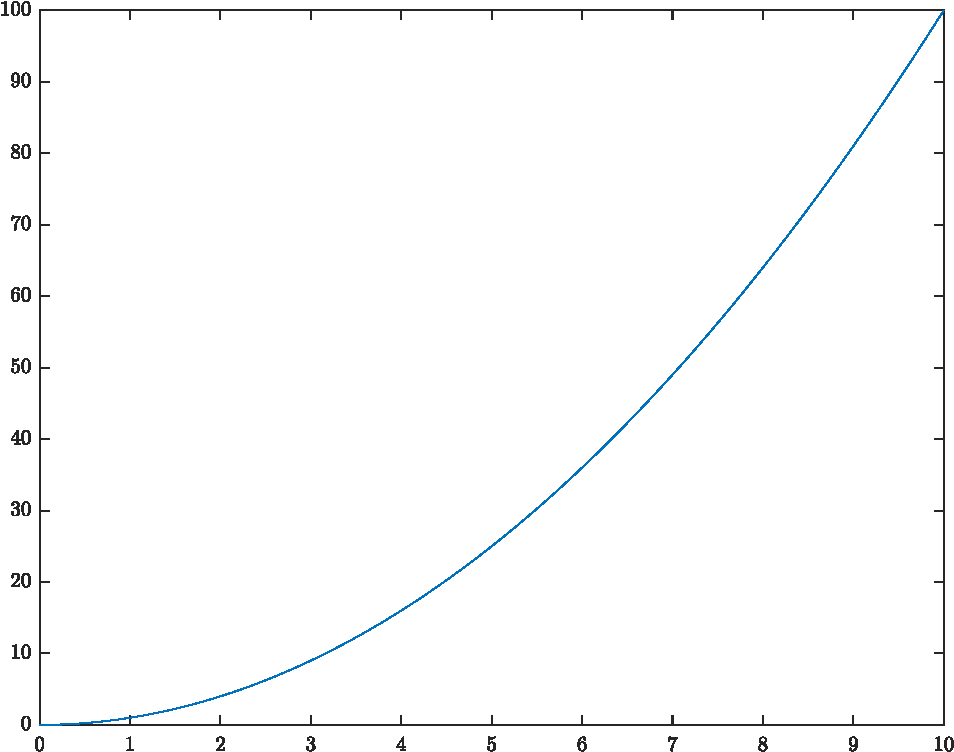
\includegraphics{gr-matlab.pdf}

This is the |misc/gr_matlab.m| input file:
\MyI{misc/gr_matlab.m}

I typed, on Linux,
\Shell{matlab -nodisplay -nodesktop -nosplash -r gr\_matlab}
in the |misc| subdirectory
to make the |graphics/gr-matlab.pdf| output file.
\end{VerbatimOut}

\MyIO


\begin{VerbatimOut}{z.out}

\section{\protect\METAPOSTLogo\ programming language}
\index{METAPOST@\METAPOSTLogo}  
\todoindex{\METAPOSTLogo}

\lightgreen{\MetaPostLogo\ uses \LaTeX\ fonts.}
\todoindex{\MetaPostLogo}

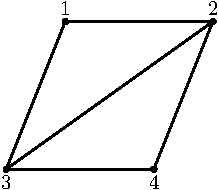
\includegraphics{gr-metapost-kim-1.pdf}
\hspace*{0.1truein}
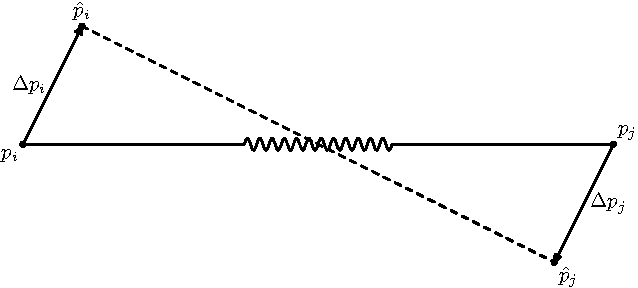
\includegraphics{gr-metapost-kim-2.pdf}

This is the |misc/gr-metapost-kim.mp| input file:
\MyI{misc/gr-metapost-kim.mp}

I typed, on Linux,\\
\hspace*{3\parindent}\Shell{mpost gr-metapost-kim}\\
\hspace*{3\parindent}\Shell{epstopdf gr-metapost-kim-1.mps;  epstopdf gr-metapost-kim-2.mps}\\
\hspace*{3\parindent}\Shell{mv -i gr-metapost-kim-1.pdf gr-metapost-kim-2.pdf ../graphics}\\
to run MetaPost and make two PDF files, |gr-metapost-kim-1.pdf| and |gr-metapost-kim-2.pdf|,
and move them to the graphics subfolder.
\end{VerbatimOut}

\MyIO


\begin{VerbatimOut}{z.out}

\subsection{Tally example}
\label{ss:tally-example}

Whenever I use files with numbers in them I like to put leading zeros
in the names so they will be listed in order in the directory.

These 20 graphics (|gr-metapost-tally-01.pdf| through |gr-metapost-tally-20.pdf|)

\vspace*{6pt}

{%
  % Let * represent zero or more spaces!
  % Method 1: \def\g#1{ requires using \g*{10} for 10.
  %           Two shifted characters, { and } are needed.
  % Method 2: \def\g#1/{ requires using \g*10/ for 10.
  %           One unshifted character, / is needed.
  \def\g#1/{\includegraphics[scale=0.5]{gr-metapost-tally-#1.pdf}}%

  % Note that tabular* instead of tabular is used below.
  %   The {\textwidth} makes the total width of the table the width
  % of the printed area of the page.
  %   The @{\kern2\parindent} puts blank space the width of two
  % paragraph indents before the first column.
  %   The @{extracolsep{\fill}} adds \fill space between all subsequent
  % columns.
  %   The lll left justifies the next three columns.
  % after the column.
  %   The @{\kern2\parindent} puts blank space the width of two
  % paragraph indents before the first column.
  \begin{tabular*}{\textwidth}{@{\kern2\parindent}@{\extracolsep{\fill}}lll@{\kern2\parindent}}%
    \g 01/& \g 02/& \g 03/\\
    \g 04/& \g 05/& \g 06/\\
    \g 07/& \g 08/& \g 09/\\
    \g 10/& \g 11/& \g 12/\\
    \g 13/& \g 14/& \g 15/\\
    \g 16/& \g 17/& \g 18/\\
    \g 19/& \g 20/\\
  \end{tabular*}%
}
\noindent were produced by

\MyI{misc/gr-metapost-tally.mp}

\end{VerbatimOut}

\MyIO


\begin{VerbatimOut}{z.out}
\section{Python programming language}
\ix{Python programming language}

\lightgreen{Python can be set up to use \LaTeX\ fonts.}

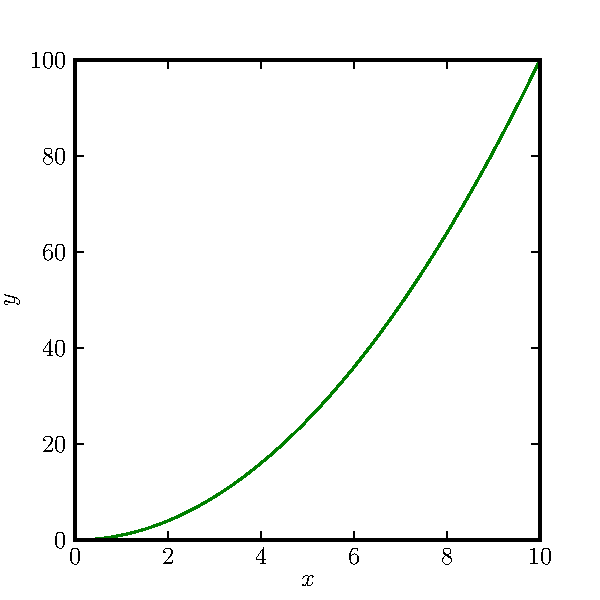
\includegraphics{gr-python2.pdf}

This is the |misc/gr-python2.py| input file:
\MyI{misc/gr-python2.py}

I typed, on Linux,
\Shell{./gr-python2.py}
in the |misc| subdirectory
to make the |graphics/gr-py|\\
|thon2.pdf| output file.
\end{VerbatimOut}

\MyIO



\begin{VerbatimOut}{z.out}

\section{R programming language}
\ix{R programming language}

\lightgreen{R can be set up to use \LaTeX\ fonts.}

% Created by tikzDevice version 0.6.2-92-0ad2792 on 2021-11-24 17:04:02
% !TEX encoding = UTF-8 Unicode
\begin{tikzpicture}[x=1pt,y=1pt]
\definecolor[named]{fillColor}{rgb}{1.00,1.00,1.00}
\path[use as bounding box,fill=fillColor,fill opacity=0.00] (0,0) rectangle (361.35,361.35);
\begin{scope}
\path[clip] ( 49.20, 61.20) rectangle (336.15,312.15);
\definecolor[named]{drawColor}{rgb}{0.00,0.00,0.00}

\path[draw=drawColor,line width= 0.4pt,line join=round,line cap=round] ( 59.83, 70.49) --
	( 62.48, 70.52) --
	( 65.14, 70.59) --
	( 67.80, 70.70) --
	( 70.46, 70.87) --
	( 73.11, 71.08) --
	( 75.77, 71.33) --
	( 78.43, 71.63) --
	( 81.08, 71.98) --
	( 83.74, 72.38) --
	( 86.40, 72.82) --
	( 89.05, 73.31) --
	( 91.71, 73.84) --
	( 94.37, 74.42) --
	( 97.03, 75.05) --
	( 99.68, 75.72) --
	(102.34, 76.44) --
	(105.00, 77.21) --
	(107.65, 78.02) --
	(110.31, 78.88) --
	(112.97, 79.79) --
	(115.62, 80.74) --
	(118.28, 81.74) --
	(120.94, 82.79) --
	(123.59, 83.88) --
	(126.25, 85.02) --
	(128.91, 86.20) --
	(131.57, 87.43) --
	(134.22, 88.71) --
	(136.88, 90.04) --
	(139.54, 91.41) --
	(142.19, 92.82) --
	(144.85, 94.29) --
	(147.51, 95.80) --
	(150.16, 97.36) --
	(152.82, 98.96) --
	(155.48,100.61) --
	(158.13,102.30) --
	(160.79,104.05) --
	(163.45,105.84) --
	(166.11,107.67) --
	(168.76,109.55) --
	(171.42,111.48) --
	(174.08,113.46) --
	(176.73,115.48) --
	(179.39,117.55) --
	(182.05,119.66) --
	(184.70,121.82) --
	(187.36,124.03) --
	(190.02,126.28) --
	(192.68,128.58) --
	(195.33,130.93) --
	(197.99,133.32) --
	(200.65,135.76) --
	(203.30,138.25) --
	(205.96,140.78) --
	(208.62,143.36) --
	(211.27,145.99) --
	(213.93,148.66) --
	(216.59,151.38) --
	(219.24,154.14) --
	(221.90,156.96) --
	(224.56,159.81) --
	(227.22,162.72) --
	(229.87,165.67) --
	(232.53,168.67) --
	(235.19,171.71) --
	(237.84,174.80) --
	(240.50,177.94) --
	(243.16,181.12) --
	(245.81,184.35) --
	(248.47,187.63) --
	(251.13,190.95) --
	(253.78,194.32) --
	(256.44,197.74) --
	(259.10,201.20) --
	(261.76,204.71) --
	(264.41,208.26) --
	(267.07,211.86) --
	(269.73,215.51) --
	(272.38,219.21) --
	(275.04,222.95) --
	(277.70,226.73) --
	(280.35,230.57) --
	(283.01,234.45) --
	(285.67,238.38) --
	(288.32,242.35) --
	(290.98,246.37) --
	(293.64,250.43) --
	(296.30,254.55) --
	(298.95,258.71) --
	(301.61,262.91) --
	(304.27,267.16) --
	(306.92,271.46) --
	(309.58,275.81) --
	(312.24,280.20) --
	(314.89,284.64) --
	(317.55,289.12) --
	(320.21,293.65) --
	(322.87,298.23) --
	(325.52,302.86);
\end{scope}
\begin{scope}
\path[clip] (  0.00,  0.00) rectangle (361.35,361.35);
\definecolor[named]{drawColor}{rgb}{0.00,0.00,0.00}

\path[draw=drawColor,line width= 0.4pt,line join=round,line cap=round] ( 59.83, 61.20) -- (325.52, 61.20);

\path[draw=drawColor,line width= 0.4pt,line join=round,line cap=round] ( 59.83, 61.20) -- ( 59.83, 55.20);

\path[draw=drawColor,line width= 0.4pt,line join=round,line cap=round] (112.97, 61.20) -- (112.97, 55.20);

\path[draw=drawColor,line width= 0.4pt,line join=round,line cap=round] (166.11, 61.20) -- (166.11, 55.20);

\path[draw=drawColor,line width= 0.4pt,line join=round,line cap=round] (219.24, 61.20) -- (219.24, 55.20);

\path[draw=drawColor,line width= 0.4pt,line join=round,line cap=round] (272.38, 61.20) -- (272.38, 55.20);

\path[draw=drawColor,line width= 0.4pt,line join=round,line cap=round] (325.52, 61.20) -- (325.52, 55.20);

\node[text=drawColor,anchor=base,inner sep=0pt, outer sep=0pt, scale=  1.00] at ( 59.83, 39.60) {0};

\node[text=drawColor,anchor=base,inner sep=0pt, outer sep=0pt, scale=  1.00] at (112.97, 39.60) {2};

\node[text=drawColor,anchor=base,inner sep=0pt, outer sep=0pt, scale=  1.00] at (166.11, 39.60) {4};

\node[text=drawColor,anchor=base,inner sep=0pt, outer sep=0pt, scale=  1.00] at (219.24, 39.60) {6};

\node[text=drawColor,anchor=base,inner sep=0pt, outer sep=0pt, scale=  1.00] at (272.38, 39.60) {8};

\node[text=drawColor,anchor=base,inner sep=0pt, outer sep=0pt, scale=  1.00] at (325.52, 39.60) {10};

\path[draw=drawColor,line width= 0.4pt,line join=round,line cap=round] ( 49.20, 70.49) -- ( 49.20,302.86);

\path[draw=drawColor,line width= 0.4pt,line join=round,line cap=round] ( 49.20, 70.49) -- ( 43.20, 70.49);

\path[draw=drawColor,line width= 0.4pt,line join=round,line cap=round] ( 49.20,116.97) -- ( 43.20,116.97);

\path[draw=drawColor,line width= 0.4pt,line join=round,line cap=round] ( 49.20,163.44) -- ( 43.20,163.44);

\path[draw=drawColor,line width= 0.4pt,line join=round,line cap=round] ( 49.20,209.91) -- ( 43.20,209.91);

\path[draw=drawColor,line width= 0.4pt,line join=round,line cap=round] ( 49.20,256.38) -- ( 43.20,256.38);

\path[draw=drawColor,line width= 0.4pt,line join=round,line cap=round] ( 49.20,302.86) -- ( 43.20,302.86);

\node[text=drawColor,rotate= 90.00,anchor=base,inner sep=0pt, outer sep=0pt, scale=  1.00] at ( 34.80, 70.49) {0};

\node[text=drawColor,rotate= 90.00,anchor=base,inner sep=0pt, outer sep=0pt, scale=  1.00] at ( 34.80,116.97) {20};

\node[text=drawColor,rotate= 90.00,anchor=base,inner sep=0pt, outer sep=0pt, scale=  1.00] at ( 34.80,163.44) {40};

\node[text=drawColor,rotate= 90.00,anchor=base,inner sep=0pt, outer sep=0pt, scale=  1.00] at ( 34.80,209.91) {60};

\node[text=drawColor,rotate= 90.00,anchor=base,inner sep=0pt, outer sep=0pt, scale=  1.00] at ( 34.80,256.38) {80};

\node[text=drawColor,rotate= 90.00,anchor=base,inner sep=0pt, outer sep=0pt, scale=  1.00] at ( 34.80,302.86) {100};

\path[draw=drawColor,line width= 0.4pt,line join=round,line cap=round] ( 49.20, 61.20) --
	(336.15, 61.20) --
	(336.15,312.15) --
	( 49.20,312.15) --
	( 49.20, 61.20);
\end{scope}
\begin{scope}
\path[clip] (  0.00,  0.00) rectangle (361.35,361.35);
\definecolor[named]{drawColor}{rgb}{0.00,0.00,0.00}

\node[text=drawColor,anchor=base,inner sep=0pt, outer sep=0pt, scale=  1.00] at (192.68, 15.60) {$x$};

\node[text=drawColor,rotate= 90.00,anchor=base,inner sep=0pt, outer sep=0pt, scale=  1.00] at ( 10.80,186.67) {$y$};
\end{scope}
\end{tikzpicture}


This is the |misc/gr-r.R| input file:
\MyI{misc/gr-r.R}

I typed, on Linux,
\Shell{R CMD BATCH gr-r}
in the |misc| subdirectory to make the |gr-r.tex| outfile file.
\end{VerbatimOut}

\MyIO


\begin{VerbatimOut}{z.out}

\section{\TikZLogo\ \LaTeX\ package}
\index{TikZ@\TikZLogo\ \LaTeX\ package}  
\todoindex{\TikZLogo\ \LaTeX\ package}

\lightgreen{\TikZLogo\ uses \LaTeX\ fonts.}
\end{VerbatimOut}

\MyIO


\begin{VerbatimOut}{z.out}

\subsection{Clock example}
\index{clock \TikZLogo\ example}
\todoindex{clock \TikZLogo\ example}
\end{VerbatimOut}

\MyIO


\begin{VerbatimOut}{z.out}

\index{TikZ@\TikZLogo}

\hbox to\textwidth{%
  \hfil
  % The idea for this clock was originally from a Google+ posting by Afamefuna ``Ferdy'' Ibeabuchia.
  \begin{tikzpicture}
    \def\CenterRadius{0.04cm}
    \def\InnerTickRadius{3.6cm}
    \def\OuterTickRadius{3.8cm}
    % Make \LR be an abbreviation for \LabelRadius so the
    % lines below will fit within the width of the page.
    \def\LabelRadius{4.5cm}      \let\LR=\LabelRadius
    \def\HourHandRadius{2.5cm}   \def\HourHandBase{0.3cm}
    \def\MinuteHandRadius{3cm}   \def\MinuteHandBase{0.4cm}
    \def\SecondHandRadius{3.5cm} \def\SecondHandBase{0.5cm}
    \def\DS{\displaystyle}
    \fill (0,0) circle (\CenterRadius);
    \foreach \i in {0,30,...,330}
    \draw (\i:\InnerTickRadius)--(\i:\OuterTickRadius);
    \node at (  0:\LR) {$\DS \qquad \sqrt9 + 9 - 9$};        %  3
    \node at ( 30:\LR) {$\DS \frac{9+9}9$};                  %  2
    \node at ( 60:\LR) {$\DS \frac{\sqrt9\sqrt9}9$};         %  1
    \node at ( 90:\LR) {$\DS 9 + \frac9{\sqrt9}$};           % 12
    \node at (120:\LR) {$\DS \frac{99}9$};                   % 11
    \node at (150:\LR) {$\DS 9 + \frac99$};                  % 10
    \node at (180:\LR) {$\DS \sqrt[\scriptstyle 9]{9^9}$};   %  9
    \node at (210:\LR) {$\DS 9 - \frac99$};                  %  8
    \node at (240:\LR) {$\DS 9 - \sqrt9 + \lceil.9\rceil$};  %  7
    \node at (270:\LR) {$\DS 9 - \frac9{\sqrt9}$};           %  6
    \node at (300:\LR) {$\DS \sqrt9\,! - \frac99$};          %  5
    \node at (330:\LR) {$\DS \sqrt9 + \frac99$};             %  4
    % In the following
    %   ABBREVIATION    DESCRIPTION
    %   deg             degrees
    %   min             minutes
    %   sec             seconds
    % for second hand:
    %   (9 sec/60 sec) * 360 deg = 54 deg;
    %   90 deg - 54 deg = 36 deg
    \draw[rotate around={36:(0,0)}]
      (-\SecondHandBase,\SecondHandBase) -- (\SecondHandRadius,0)
        -- (-\SecondHandBase,-\SecondHandBase) -- cycle;
    % for minute hand:
    %   (9 min/60 min) * 360 deg = 54 deg;
    %   90 deg - 54 deg = 36 deg
   \draw[rotate around={36:(0,0)}]
     (-\MinuteHandBase,\MinuteHandBase) -- (\MinuteHandRadius,0)
       -- (-\MinuteHandBase,-\MinuteHandBase) -- cycle;
    % for hour hand:
    %   (9 min * (60 sec/1 min)) + 9 sec) / 3600 sec
    %     = 549 sec / 3600 sec = 0.1525
    %   The hour hand is 0.1525 of the way from 9:00 to 10:00.
    %   Each hour is 30 degrees on the clock, so the hour hand
    %   position is
    %     30 deg * 0.1525 = 4.575 deg past 9:00
    %   180 deg - 4.575 deg = 175.425 deg
    \draw[rotate around={175.425:(0,0)}]
      (-\HourHandBase,\HourHandBase) -- (\HourHandRadius,0)
      -- (-\HourHandBase,-\HourHandBase) -- cycle;
  \end{tikzpicture}
  \hfil
}
\end{VerbatimOut}

\MyIO


\begin{VerbatimOut}{z.out}

\newpage

\subsection{Counter example}
\index{Counter \TikZLogo\ example}
\todoindex{Counter \TikZLogo\ example}

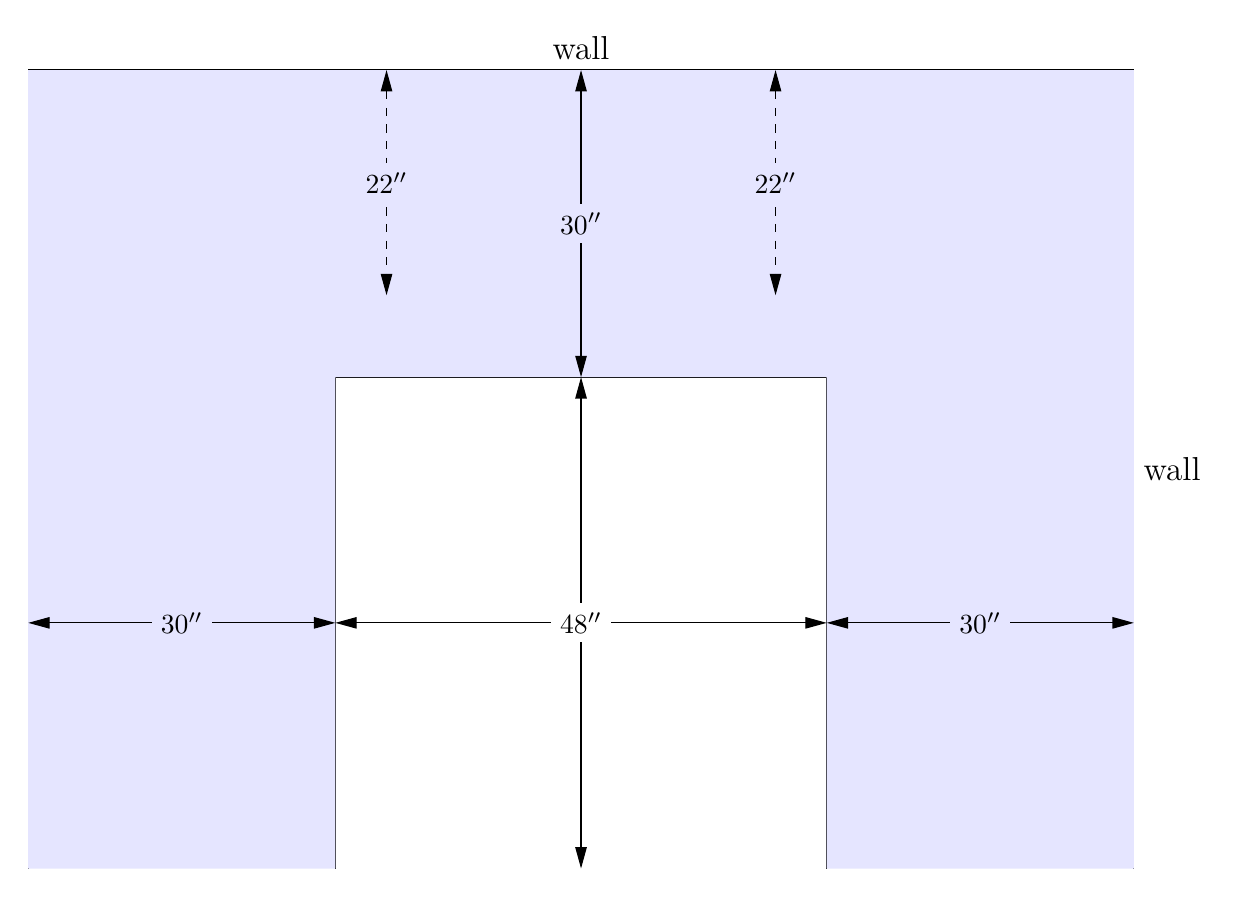
\begin{tikzpicture}[scale=0.13]
  % Define points.
  \coordinate   (p11) at (  0, 78);
    \coordinate (p14) at ( 35, 78);
    \coordinate (p15) at ( 54, 78);
    \coordinate (p16) at ( 73, 78);
    \coordinate (p19) at (108, 78);
  \coordinate   (p24) at ( 35, 67);
    \coordinate (p26) at ( 73, 67);
  \coordinate   (p35) at ( 54, 63);
  \coordinate   (p44) at ( 35, 56);
    \coordinate (p46) at ( 73, 56);
  \coordinate   (p53) at ( 30, 48);
    \coordinate (p55) at ( 54, 48);
    \coordinate (p57) at ( 78, 48);
  \coordinate   (p69) at (108, 39);
  \coordinate   (p71) at (  0, 24);
    \coordinate (p72) at ( 15, 24);
    \coordinate (p73) at ( 30, 24);
    \coordinate (p75) at ( 54, 24);
    \coordinate (p77) at ( 78, 24);
    \coordinate (p78) at ( 93, 24);
    \coordinate (p79) at (108, 24);
  \coordinate   (p81) at (  0,  0);
    \coordinate (p83) at ( 30,  0);
    \coordinate (p85) at ( 54,  0);
    \coordinate (p87) at ( 78,  0);
    \coordinate (p89) at (108,  0);
  % Put "wall" above drawing.
  \draw (p15) node[above] {\large wall};
  % Plot outer edge.
  \draw (p81) -- (p11) -- (p19) -- (p89);
  % Plot inner edge.
  \draw (p83) -- (p53) -- (p57) -- (p87);
  % Color the counter. 
  \fill[blue!10] (p81) -- (p11) -- (p19) -- (p89) -- (p87) -- (p57) -- (p53) -- (p83) -- cycle;
  % Vertical measurement lines.
  \draw[dashed, arrows = {Stealth[inset=0pt, angle=30:8pt]-Stealth[inset=0pt, angle=30:8pt]}]
    (p14) -- (p44);
  \draw (p24) node[fill=blue!10] {$22''$};
  \draw[arrows = {Stealth[inset=0pt, angle=30:8pt]-Stealth[inset=0pt, angle=30:8pt]}] (p15) -- (p55);
  \draw (p35) node[fill=blue!10] {$30''$};
  \draw[dashed, arrows = {Stealth[inset=0pt, angle=30:8pt]-Stealth[inset=0pt, angle=30:8pt]}]
    (p16) -- (p46);
  \draw (p26) node[fill=blue!10] {$22''$};
  \draw[arrows = {Stealth[inset=0pt, angle=30:8pt]-Stealth[inset=0pt, angle=30:8pt]}] (p55) -- (p85);
  % Horizontal measurement lines.
  \draw[arrows = {Stealth[inset=0pt, angle=30:8pt]-Stealth[inset=0pt, angle=30:8pt]}] (p71) -- (p73);
  \draw (p72) node[fill=blue!10] {$30''$};
  \draw[arrows = {Stealth[inset=0pt, angle=30:8pt]-Stealth[inset=0pt, angle=30:8pt]}] (p73) -- (p77);
  \draw (p75) node[fill=white] {$48''$};
  \draw[arrows = {Stealth[inset=0pt, angle=30:8pt]-Stealth[inset=0pt, angle=30:8pt]}] (p77) -- (p79);
  \draw (p78) node[fill=blue!10] {$30''$};
  % Put "wall" to the right of drawing.
  \draw (p69) node[right] {\large wall};
\end{tikzpicture}
\end{VerbatimOut}

\MyIO


\begin{VerbatimOut}{z.out}

\subsection{Fourier transform example}
\index{Fourier transform \TikZLogo\ example}
\todoindex{Fourier transform \TikZLogo\ example}
  
The Fourier transform decomposes a function
into the frequencies that make it up.
The inverse Fourier transformation combines the contributions
of all the different frequencies to recover the original function.

(Mark Senn {\tt\char'074}mark@purdue.edu{\tt\char'076} wrote sales@aavos.be on 2021-09-03
to ask permission
to use
\href{https://aavos.eu/glossary/fourier-transform/}{Fourier transform}
as the starting point
for an example \TikZLogo\ figure.  
Dominique Demurie {\tt\char'074}sales@aavos.be{\tt\char'076} replied
on 2021-09-06 with
``I think it is not an original drawing from us either.
We had it for years on our website,
but I cannot remember where we got it from.
We don't mind you using it for a thesis.'')

% Run this with
%     pdflatex --shell-escape t
% That makes the t.table.* files.
%
% See
%     https://ctan.math.washington.edu/tex-archive/graphics/pgf/base/doc/pgfmanual.pdf
%     PAGE    TOPIC
%      655    decorations.text library to draw text 
%     1221    animations
%
% for text decorations, which includes text along a path information.
% Also see
%     https://tex.stackexchange.com/questions/427454/tikz-3dplot-and-rotation-of-coordinates
%     https://tex.stackexchange.com/questions/67573/tikz-shift-and-rotate-in-3d
%     http://tug.ctan.org/graphics/pgf/contrib/tikz-3dplot/tikz-3dplot_documentation.pdf
%     https://tex.stackexchange.com/questions/45848/rotate-node-text-and-use-relative-positioning-in-tikz
  
% was scale = 2
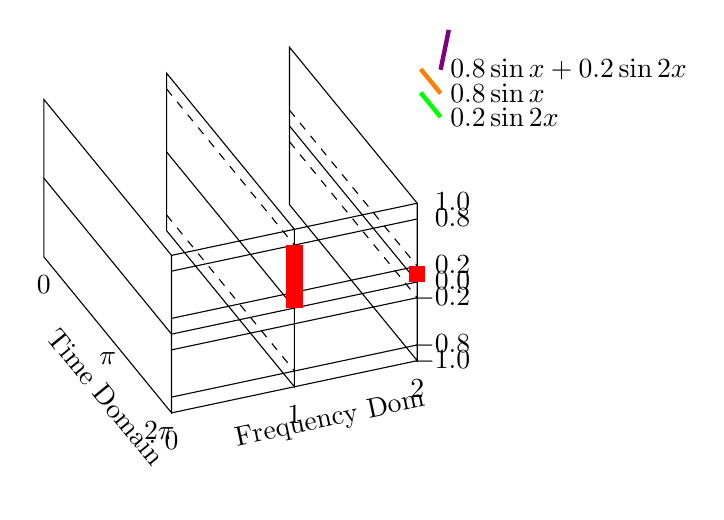
\begin{tikzpicture}[domain=0:6.283185, rotate around y=-55, scale=1]

  % total plot
  \begin{scope}[canvas is xy plane at z=0]
    \node[below=3pt] at (0,        -1) {0};
    \node[below=3pt] at (3.141593, -1) {$\pi$};
    \node[below=5pt] at (5.683185, -1) {$2\pi$};
    \draw[ultra thick,color=violet] plot[id=total,smooth] function{0.8*sin(x)+0.2*sin(8*x)};
    \draw[thin,color=black] (0,-1) -- (0,1) -- (6.283185,1) -- (6.283185,-1) -- cycle;
    \draw[thin,color=black] (0,0) -- (6.283185,0);
    \path[decorate,decoration={text along path,
% |\LARGE|
      text={Time Domain}}] (0.1,-2) -- (6.283185,-2); 
    % $s(t)$
  \end{scope}

  % tall plot
  \begin{scope}[canvas is xy plane at z=-1.5]
    \draw[dashed] (0,0.8) -- (6.283185,0.8);
    \draw[dashed] (0,-0.8) -- (6.283185,-0.8);
    \draw[thick,color=orange] plot[id=tall,smooth] function{0.8*sin(x)};
    \draw[thin,color=black] (0,-1) -- (0,1) -- (6.283185,1) -- (6.283185,-1) -- cycle;
    \draw[thin,color=black] (0,0) -- (6.283185,0);
  \end{scope}

  % short plot
  \begin{scope}[canvas is xy plane at z=-3.0]
    \draw[dashed] (0, 0.2) -- (6.283185,  0.2);
    \draw[dashed] (0,-0.2) -- (6.283185, -0.2);
    \draw[thick,color=green] plot[id=short,smooth] function{0.2*sin(2*x)};
    \draw[thin,color=black] (0,-1) -- (0,1) -- (6.283185,1) -- (6.283185,-1) -- cycle;
    \draw[thin,color=black] (0,0) -- (6.283185,0);
  \end{scope}

  % frequency plot
  \begin{scope}[canvas is zy plane at x=6.283185]
    \node[below=3pt] at ( 0.0,-1) {0};
    \node[below=3pt] at (-1.5,-1) {1};
    \node[below=3pt] at (-3.0,-1) {2};
    \draw[thin,color=black] (0,-1.0) -- (-3.0,-1.0);  \node[above=-9pt] at (-3.3,-1.0) {$-1.0$};
    \draw[thin,color=black] (0,-0.8) -- (-3.0,-0.8);  \node[above=-9pt] at (-3.3,-0.8) {$-0.8$};
    \draw[thin,color=black] (0,-0.2) -- (-3.0,-0.2);  \node[above=-9pt] at (-3.3,-0.2) {$-0.2$};
    \draw[thin,color=black] (0, 0.0) -- (-3.0, 0.0);  \node[above=-9pt] at (-3.3, 0.0) {$\phantom{-}0.0$};
    \draw[thin,color=black] (0, 0.2) -- (-3.0, 0.2);  \node[above=-9pt] at (-3.3, 0.2) {$\phantom{-}0.2$};
    \draw[thin,color=black] (0, 0.8) -- (-3.0, 0.8);  \node[above=-9pt] at (-3.3, 0.8) {$\phantom{-}0.8$};
    \draw[thin,color=black] (0, 1.0) -- (-3.0, 1.0);  \node[above=-9pt] at (-3.3, 1.0) {$\phantom{-}1.0$};
    \draw[line width=6pt,color=red] (-1.5,0) -- (-1.5,0.8);
    \draw[line width=6pt,color=red] (-3.0,0) -- (-3.0,0.2);
    \path[decorate,decoration={text along path,
% |\LARGE|
      text={Frequency Domain}}] (-0.8,-1.6) -- (-3.0,-1.6); 
    % $S(\omega)$
  \end{scope}

  %% legend
  %% Wolfram Language code:
  %%     In[1]:= ry[theta_] :=
  %%     {
  %%         {Cos[theta Degree],  0, Sin[theta Degree]},
  %%         {0,                  1, 0},
  %%         {-Sin[theta Degree], 0, Cos[theta Degree]}
  %%     }
  %%
  %%     ry[55] . {Pi, 0.7, -3.5}
  %%     # Out[] = {-1.06509, 0.7, -4.58096}
  %%     ry[55] . {(3/4)Pi, 0.7, -3.5}
  %%     # Out[] = {-1.51557, 0.7, -3.9376}

  \draw[ultra thick,color=violet] (2.45782, 1.7, -4.33538) -- (1.06509, 0.7, -4.58096);
    \node[right] at                                            (1.06509, 0.7, -4.58096) {$0.8\sin x + 0.2\sin 2x$};
  \draw[ultra thick,color=orange] ( 0.08509, 0.4, -4.58096) -- (1.06509, 0.4, -4.58096);
    \node[right] at                                            (1.06509, 0.4, -4.58096) {$0.8\sin x$};
  \draw[ultra thick,color=green]  ( 0.08509, 0.1, -4.58096) -- (1.06509, 0.1, -4.58096);
    \node[right] at                                            (1.06509, 0.1, -4.58096) {$0.2\sin 2x$};
\end{tikzpicture}
\end{VerbatimOut}

\MyIO


\begin{VerbatimOut}{z.out}

\subsection{Glider example}
\ix{Hirzel, Alex}
\index{glider \TikZLogo\ example}
\todoindex{glider \TikZLogo\ example}

The glider
is a pattern from the Game of Life,
and it's used as an emblem representing the hacker community.

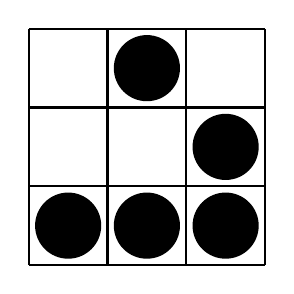
\begin{tikzpicture}[thick]
  \draw (0,0) grid (3,3);
  \foreach \c in {(0,0), (1,0), (2,0), (2,1), (1,2)}
    \fill \c + (0.5,0.5) circle (0.42);
\end{tikzpicture}
\end{VerbatimOut}

\MyIO


\begin{VerbatimOut}{z.out}

\newpage

\subsection{Tree example}
\ix{???, ???}
\index{tree \TikZLogo\ example}
\todoindex{tree \TikZLogo\ example}

{
  \def\f#1#2{$\displaystyle\frac #1#2$}
  \begin{tikzpicture}%
  [%
    level 1/.style={sibling distance=60mm},
    level 2/.style={sibling distance=30mm},
    level 3/.style={sibling distance=15mm}
  ]
    \node {\f 11}
      child {node {$\displaystyle\frac 12$}
        child {node {\f 13}
          child {node {\f 14}}
          child {node {\f 48}}
        }
        child {node {\f 32}
          child {node {\f 35}}
          child {node {\f 52}}
        }
      }
      child {node {\f 21}
        child {node {\f 23}
          child {node {\f 25}}
          child {node {\f 53}}
        }
        child {node {\f 31}
          child {node {\f 34}}
          child {node {\f 41}}
        }
      };
  \end{tikzpicture}    

\vspace*{4pt}
The node with value \f nd\\[2pt]
\indent\hspace*{4\parindent}
\begin{tabular}{@{}llll@{}}
  \bfseries with additional conditions& \bfseries has& \bfseries with value\\
  \noalign{\vspace{2pt}}
  (none)&                     left child&     \f n{{n+d}}\\
  \noalign{\vspace{12pt}}
  (none)&                     right child&    \f {{n+d}}d\\
  \noalign{\vspace{12pt}}
  $n<d$&                      parent&         \f n{{d-n}}\\
  \noalign{\vspace{12pt}}
  $n=d$&                      no parent&      (not applicable)\\
  \noalign{\vspace{12pt}}
  $n>d$&                      parent&         \f {{n-d}}d\\
\end{tabular}
}
\end{VerbatimOut}

\MyIO

\begin{VerbatimOut}{z.out}


\subsection{Yin and yang example}

This Yin and yang example was done by Thomas G. Kristensen \cite{kristensen}.
This is the ``traditional Taijitu symbol from Chinese philosophy''.
\ix{Kristensen, Thomas G.//Taijitu symbol//Yin and yang symbol}

\index{TikZ@\TikZLogo}  
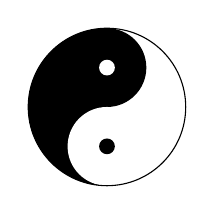
\begin{tikzpicture}
  % Yin and yang
  % Author: Thomas G. Kristensen
  
  % color one half of a unit circle                                              
  \begin{scope}
    \clip (0,0) circle (1cm);
    \fill[black] (0cm,1cm) rectangle (-1cm, -1cm);
  \end{scope}

  % fill heads                                                                   
  \fill[black] (0,0.5) circle (0.5cm);
  \fill[white] (0,-0.5) circle (0.5cm);

  % fill eyes                                                                    
  \fill[white] (0,0.5) circle (0.1cm);
  \fill[black] (0,-0.5) circle (0.1cm);

  % outer line                                                                   
  \draw (0,0) circle (1cm);

\end{tikzpicture}
\end{VerbatimOut}

\MyIO


\begin{VerbatimOut}{z.out}

\section{Wolfram Language (Mathematica uses this)}
\ix{Mathematica}
\ix{Wolfram Language}

\lightgreen{Wolfram Language can be set up to use \LaTeX\ fonts.}

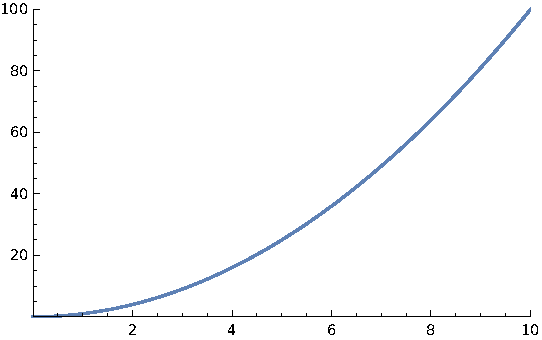
\includegraphics{gr-mathematica.pdf}

This is the |misc/gr-mathematica.ma| input file
\MyI{misc/gr-mathematica.ma}

I typed, on Linux,
\Shell{math < gr-mathematica.ma}
in the |misc| subdirectory
to make the |graphics/gr-mathematica.pdf| output file.
\end{VerbatimOut}

\MyIO


  % Ignore these references.
  %\ProvidesFile{ap-ignore-these-references.tex}[2022-10-05 ignore these references appendix]

\begin{VerbatimOut}{z.out}
\chapter{IGNORE THESE REFERENCES---THEY ARE WRONG}
\end{VerbatimOut}

\MyIO


\begin{VerbatimOut}{z.out}

You may have seen these references on the web.
Ignore them---they're wrong.

\noindent
\textbf{Purdue Online Writing Lab, IEEE Reference List}
\cite{owl}

The IEEE
(The world's largest technical professional organization
for the advancement
of technology)
has changed their references format from,
for example,

\noindent
\begin{tabular}{@{}ll@{}}
\noalign{\vspace*{6pt}}
  [1]& W. K. Chen, Linear Networks and Systems. Belmont, CA: Wadsworth Press,\\
  \multispan{2}{2003.\hfil}\\
\noalign{\vspace*{6pt}}
\noalign{\noindent to}
\noalign{\vspace*{6pt}}
  [1]& W. K. Chen, Linear Networks and Systems. Belmont, CA: Wadsworth Press,\\
  & 2003.\hfil\\
\noalign{\vspace*{6pt}}
\end{tabular}
See
\cite[page~2]{ieeedataport}.
\end{VerbatimOut}

\MyIO


% BL  @online{owl,
% BT  @misc{owl,
%     author  = {Purdue Online Writing Lab},
%     title   = {IEEE Reference List},
%     url     = {https://owl.purdue.edu/owl/research_and_citation/ieee_style/reference_list.html},
% BL  urldate = {2022-03-17},
% }
% 
% BL  @online{ieeedataport,
% BT  @misc{ieeedataport,
%     author  = {IEEEDataPort},
%     title   = {How too Cite References: IEEE Documentation Style},
%     url     = {https://ieee-dataport.org/sites/default/files/analysis/27/IEEE%20Citation%20Guidelines.pdf},
% BL  urldate = {2022-03-17},
% }  


  % Logos.
  %\ProvidesFile{ap-logos.tex}[2022-10-05 logos appendix]

\begin{VerbatimOut}{z.out}
\chapter{LOGOS}

These logos are defined in |pa-logos.sty|:

\begin{tabular}{@{}ll@{}}
  \toprule
  \bfseries Input& \bfseries Output\\
  \midrule
  % From thesis.tex
  %     \newcommand{\tabularspace}{\noalign{\vspace*{2pt}}}
  % \tabularspace
  \verb+\AMSmathLogo+& \AMSmathLogo\\[2pt]
  \verb+\BibLaTeXLogo+& \BibLaTeXLogo\\[2pt]
  \verb+\BiberLogo+& \BiberLogo\\[2pt]
  \verb+\CalligraphicAMSLaTeXLogo+& \CalligraphicAMSLaTeXLogo\\[2pt]
  \verb+\CircuiTikZLogo+& \CircuiTikZLogo\\[2pt]
  \verb+\CTANLogo{\texttt{CTAN}\xspace}+& \CTANLogo\\[2pt]
  \verb+\LaTeXLogo+& \LaTeXLogo\\[2pt]
  \verb+\LuaLaTeXLogo+& \LuaLaTeXLogo\\[2pt]
  \verb+\METAFONTLogo+& \METAFONTLogo\\[2pt]
  \verb+\METAPOSTLogo+& \METAPOSTLogo\\[2pt]
  \verb+\MetaPostLogo+& \MetaPostLogo\\[2pt]
  \verb+\NonCalligraphicAMSLaTeXLogo+& \NonCalligraphicAMSLaTeXLogo\\[2pt]
  \verb+\PurdueThesisLogo+& \PurdueThesisLogo\\[2pt]
  \verb+\PuThLogo+& \PuThLogo\\[2pt]
  \verb+\TeXLogo+& \TeXLogo\\[2pt]
  \verb+\TeXLiveLogo+& \TeXLiveLogo\\[2pt]
  \verb+\TikZLogo+& \TikZLogo\\[2pt]
  \verb+\TEXUsersGroupLogo+& \TeXUsersGroupLogo\\[2pt]
  \verb+\TUGboatLogo+& \TUGboatLogo\\[2pt]
  \bottomrule
\end{tabular}
\end{VerbatimOut}

\MyIO


  % Miscellaneous.
  %\ProvidesFile{ap-miscellaneous.tex}[2022-10-05 miscellaneous appendix]

\begin{VerbatimOut}{z.out}
\chapter{MISCELLANEOUS}
\ix{miscellaneous//Miscellaneous appendix}
\end{VerbatimOut}

\MyIO


\begin{VerbatimOut}{z.out}
Demonstrate using a long Hungarian umlaut
(double acute)
(\H{o})
in text and bibligraphy
\cite{erdos1992}.
\end{VerbatimOut}

\MyIO

  
  % Numbers and Units.
  %\ProvidesFile{ap-numbers-and-units.tex}[2022-10-05 numbers and units appendix]

%  Primary sources:
%      See https://www.bipm.org/utils/common/pdf/si-brochure/SI-Brochure-9-EN.pdf.
%      See https://www.nist.gov/pml/special-publication-811/nist-guide-si-chapter-4-two-classes-si-units-and-si-prefixes.
%
%  Notes:
%      See https://www.iso.org/standard/60241.html.

% Historic Vote Ties Kilogram and Other Units to Natural Constants
% NIST
% https://www.nist.gov/news-events/news/2018/11/historic-vote-ties-kilogram-and-other-units-natural-constants
% created 2018-11-16
% updated 2018-12-21
% last retrieved 2018-12-22

% https://www.bipm.org/utils/common/pdf/CGPM-2018/26th-CGPM-Resolutions.pdf
% Resolutions adopted
% 26^e CGPM
% Versailes
% 13--16 November 2018
% last retrieved 2018-12-30

% author Joseph Wright
% date 2018-05-17
% retrieved 2018-12-29
% url ftp://ftp.dante.de/tex-archive/macros/latex/exptl/siunitx/siunitx.pdf


\begin{VerbatimOut}{z.out}
\chapter{NUMBERS AND UNITS}
\end{VerbatimOut}

\MyIO


\begin{VerbatimOut}{z.out}

Note to self: scientific prefixes, scientific suffixes, tables.

The puthesis 2.0 and after documentclass uses the siunitx
package with some extra definitions in the puthesis.cls
file to do numbers and units.
\end{VerbatimOut}

\MyIO


\begin{VerbatimOut}{z.out}

\section{Number Examples}
\end{VerbatimOut}

\MyIO


\begin{VerbatimOut}{z.out}
\noindent\begin{tabular}{@{}lll@{}}
  \bfseries Input& \bfseries Output& \bfseries Comment\\
  \tabularspace
  \verb+\num{-0.12345}+& \num{-0.12345}& note the small space after the ``3''\\
  \verb+\num{-0.1234}+&
    \num{-0.1234}&
    note no space between the ``3'' and ``4''\\
  \verb+\num{-.123}+& \num{-.123}& the ``0.'' is inserted automatically\\
  \verb+\num{123}+& \num{123}\\
  \verb+\num{1234}+& \num{1234}\\
  \verb+\num{12345}+& \num{12345}& note the small space after the ``2''\\
  \verb+\num{2e4}+& \num{2e4}\\
  \verb+\num{e5}+& \num{e5}\\
  \verb+\num{2.34567e6}+&
    \num{2.34567e6}&
    note the small space after the ``5''\\
\end{tabular}
\end{VerbatimOut}

\MyIO


\begin{VerbatimOut}{z.out}

\section{Unit Examples}
\end{VerbatimOut}

\MyIO


\begin{VerbatimOut}{z.out}

See page~\pageref{se:Complete-List-of-Units}
for the complete list
of units defined by \PurdueThesisLogo.

\noindent\begin{tabular}{@{}lll@{}}
  \bfseries Input& \bfseries Output& \bfseries Comment\\
  \tabularspace
  \verb+\si{\kg}+& \si{\kg}& kilogram\\
  \verb+\si{\m}+& \si{\m}& meter\\
  \verb+\si{\kg\per\m\squared}+&
    \si{\kg\per\m\squared}&
    \(= \si{\kg}/\si{\m\squared}\)\\
\end{tabular}
\end{VerbatimOut}

\MyIO


\begin{VerbatimOut}{z.out}

\section{Combined Number and Unit Examples}
\end{VerbatimOut}

\MyIO


\begin{VerbatimOut}{z.out}
\begin{tabular}{@{}lll@{}}
  \bfseries Input& \bfseries Output& \bfseries Comment\\
  \tabularspace
  \verb+\SI{12}{\kg}+& \SI{12}{\kg}& 12 kilograms\\
  \verb+\SI{34}{\m}+&  \SI{34}{\m}& 34 meters\\
  % The next input line is too wide for the margins
  % so I'm splitting it into pieces.
  \verb+\SI{4.5e3}{\kg\per\m\squared}+&
    \SI{4.5e3}{\kg\per\m\squared}&
    \(= \num{4.5e3}\,\si{\kg}/\si{\m\squared}\)\\
\end{tabular}
\end{VerbatimOut}

\MyIO


\begin{VerbatimOut}{z.out}

How many seconds are in a non-leap year that does not have any leap seconds?
% I tried several things and couold not get \cancel to work with \per.
% Mark Senn    2019-12-29
\begin{align*}
           \frac{\SI{365}{\cancel\d}}{\si{\y}}
    \times \frac{\SI{24}{\cancel\h}}{\si{\cancel\d}}
    \times \frac{\SI{60}{\cancel\min}}{\si{\cancel\h}}         
    \times \frac{\SI{60}{\s}}{\si{\cancel\min}}         
    % From http://www.emerson.emory.edu/services/latex/latex_119.html
    %     Spacing in Math Mode
    %     In a math environment, LaTeX ignores the spaces you type
    %     and puts in the spacing that it thinks is best. LaTeX formats
    %     mathematics the way it's done in mathematics texts. If you
    %     want different spacing, LaTeX provides the following four
    %     commands for use in math mode:
    %         \; - a thick space
    %         \: - a medium space
    %         \, - a thin space
    %         \! - a negative thin space
    & = \num{31536000}\;\frac{\si{\s}}{\si{\y}}\\
    & = \SI{31536000}{\s\per\y}\\
    & \approx \SI{3e7}{\s\per\y}\\
    & \approx \text{30 million\,}\si{\s\per\y}\\
\end{align*}
\end{VerbatimOut}

\MyIO


\begin{VerbatimOut}{z.out}

\section{Binary Prefixes}
\end{VerbatimOut}

\MyIO


\begin{VerbatimOut}{z.out}

The \verb+\kibi+ \ldots \verb+\yobi+
commands are defined immediately after the \verb+\usepackage{siunitx}+ command
in the PurdueThesis.cls file.
\end{VerbatimOut}

\MyIO


\begin{VerbatimOut}{z.out}

\newcolumntype{m}{>{$}r<{$}}  % math mode version of "r" column type
\renewcommand{\t}[4]{\(2^{#1}\) bytes is a #2, \(10^{#3}\) bytes is a #4}
\begin{tabular}{@{}mllll@{}}
  \multicolumn{1}{l}{\bfseries Power}&
    \bfseries Prefix&
    \bfseries Symbol&
    \bfseries Command&
    \bfseries Comment\\
  \tabularspace
  10& kibi& \unit{\kibi\nounit}& \verb+\si{\kibi}+& \t{10}{KB}{3}{KiB}\\
  20& mebi& \unit{\mebi\nounit}& \verb+\si{\mebi}+& \t{20}{MB}{6}{MiB}\\
  30& gibi& \unit{\gibi\nounit}& \verb+\si{\gibi}+& \t{30}{GB}{9}{GiB}\\
  40& tebi& \unit{\tebi\nounit}& \verb+\si{\tebi}+& \t{40}{TB}{12}{TiB}\\
  50& pebi& \unit{\pebi\nounit}& \verb+\si{\pebi}+& \t{50}{PB}{15}{PiB}\\
  60& exbi& \unit{\exbi\nounit}& \verb+\si{\exbi}+& \t{60}{EB}{18}{EiB}\\
  70& zebi& \unit{\zebi\nounit}& \verb+\si{\zebi}+& \t{70}{ZB}{21}{ZiB}\\
  80& yobi& \unit{\yobi\nounit}& \verb+\si{\yobi}+& \t{80}{YB}{24}{YiB}\\
\end{tabular}
\end{VerbatimOut}

\MyIO


\begin{VerbatimOut}{z.out}

\section{Decimal Prefixes}
\end{VerbatimOut}

\MyIO

\begin{VerbatimOut}{z.out}

\newcolumntype{m}{>{$}r<{$}}  % math mode version of "r" column type
\begin{tabular}{@{}mllll@{}}
  \multicolumn{1}{l}{\bfseries Power}&
    \bfseries Prefix&
    \bfseries Symbol&
    \bfseries Command&
    \bfseries Comment\\
  \tabularspace
  -24& yocto& \unit{\yocto\nounit}& \verb+\si{\yocto}+\\
  -21& zepto& \unit{\zepto\nounit}& \verb+\si{\zepto}+\\
  -18& atto&  \unit{\atto\nounit}&  \verb+\si{\atto}+\\
  -15& femto& \unit{\femto\nounit}& \verb+\si{\femto}+\\
  -12& pico&  \unit{\pico\nounit}&  \verb+\si{\pico}+\\
   -9& nano&  \unit{\nano\nounit}&  \verb+\si{\nano}+\\
   -6& micro& \unit{\micro\nounit}& \verb+\si{\micro}+\\
   -3& milli& \unit{\milli\nounit}& \verb+\si{\milla}+\\
   -2& centi& \unit{\centi\nounit}& \verb+\si{\centi}+\\
   -1& deci&  \unit{\deci\nounit}&  \verb+\si{\deci}+\\
    1& deca&  \unit{\deca\nounit}&  \verb+\si{\deca}+\\
    1& deka&  \unit{\deka\nounit}&  \verb+\si{\deka}+& same as \verb+\si{\deca}+\\
    2& hecto& \unit{\hecto\nounit}& \verb+\si{\hecto}+\\
    3& kilo&  \unit{\kilo\nounit}&  \verb+\si{\kilo}+\\
    6& mega&  \unit{\mega\nounit}&  \verb+\si{\mega}+\\
    9& giga&  \unit{\giga\nounit}&  \verb+\si{\giga}+\\
   12& tera&  \unit{\tera\nounit}&  \verb+\si{\tera}+\\
   15& peta&  \unit{\peta\nounit}&  \verb+\si{\peta}+\\
   18& exa&   \unit{\exa\nounit}&   \verb+\si{\exa}+\\
   21& zetta& \unit{\zetta\nounit}& \verb+\si{\zetta}+\\
   24& yotta& \unit{\yotta\nounit}& \verb+\si{\yotta}+\\
\end{tabular}
\end{VerbatimOut}

\MyIO


\begin{VerbatimOut}{z.out}

\section{SI Units}
\end{VerbatimOut}

\MyIO


\begin{VerbatimOut}{z.out}

The International System of Units
(SI)
% !!! Doing
% !!!     \include{tipa}
% !!! in thesis.tex so \textprimstress works
% !!! apparently causes problems with math commands.
% !!! Figure out why the following doesn't work later.
% (%
%   SI,
%   abbreviated from the French Syst\`eme International
%   (d\textprimstress unit\'es)%
% )
is the modern form of the metric system.
There are seven SI base units:

\hspace{40pt}
\begin{tabular}{@{}lll@{}}
  \tabularspace
  \bfseries Name& \bfseries Unit Of&         \bfseries Symbol\\
  \tabularspace
  ampere&         electrical current&        \si{\ampere}\\
  candela&        luminous intensity&        \si{\candela}\\
  kelvin&         thermodynamic temperature& \si{\kelvin}\\
  kg&             mass&                      \si{\kilogram}\\
  meter&          length&                    \si{\meter}\\
  mole&           amount of substance&       \si{\mole}\\
  second&         time&                      \si{\second}\\
\end{tabular}
\end{VerbatimOut}

\MyIO


\begin{VerbatimOut}{z.out}

\section{Complete List of Units}
\label{se:Complete-List-of-Units}
\end{VerbatimOut}

\MyIO

\begin{VerbatimOut}{z.out}

{%
  \ZZbaselinestretch{1}
  \newcommand\vsp{\noalign{\vspace*{6pt}}}
  % From
  % https://tex.stackexchange.com/questions/31508/flushleft-with-p-option-in-tabular
  %     It's necessary to use the \arraybackslash in the last column,
  %     otherwise \\ would not end the table row.  You can use \newline
  %     to end lines in the last column cells (and the regular \\ in
  %     the other column cells).
  %     ...
  %     If you need it often, consider defining a new column type using
  %     array features, as I did here:
  %         \newcolumntype{P}[1]{>{\raggedright\arraybackslash}p{#1}}
  \newcolumntype{P}[1]{>{\raggedright\arraybackslash}p{#1}}%
% \begin{longtable}{@{}P{1.4in}P{1in}llP{1.8in}@{}}
% \begin{longtable}{@{}P{1in}P{1in}llP{1.8in}@{}}
% \begin{longtable}{@{}P{1.2in}P{1in}llP{1.8in}@{}}
% \begin{longtable}{@{}P{90.72pt}P{1in}llP{1.8in}@{}}  % 1.2in (86.72pt) + 4pt = 90.72pt
  \begin{longtable}{@{}P{1.4in}P{1in}llP{1.8in}@{}}% 1.2in (86.72pt) + 4pt = 90.72pt
      \caption{Units and Corresponding Symbols}\\
      \bfseries Name&
        \bfseries Unit Of&
        \bfseries Symbol&
        \bfseries Command&
        \bfseries Is equal to\\
      \vsp
    \endfirsthead
      \caption[]{~\emph{continued}}\\
      \bfseries Name&
        \bfseries Unit Of&
        \bfseries Symbol&
        \bfseries Command&
        \bfseries Is equal to\\
      \vsp
    \endhead
      \vsp
      % I don't know why the \hspace*{-7.5mm} was
      % needed to center this horizontally.
      \multicolumn{5}{@{}c@{}}{\hspace*{-7.5mm}\emph{continued on next page}}%
    \endfoot    
    \endlastfoot
    ampere&
      electrical current&
      \si{\A}&
      \verb+\si{\A}+&
      (SI base unit)\\
    \quad picoampere&
      \ditto&
      \si{\pA}&
      \verb+\si{\pA}+&
      \SI{e-12}{\A}\\ 
    \quad nanoampere&
      \ditto&
      \si{\nA}&
      \verb+\si{\nA}+&
      \SI{e-9}{\A}\\
    \quad microampere&
      \ditto&
      \si{\uA}&
      \verb+\si{\uA}+&
      \SI{e-6}{\A}\\
    \quad milliampere&
      \ditto&
      \si{\mA}&
      \verb+\si{\mA}+&
      \SI{e-3}{\A}\\
    \quad kiloampere&
      \ditto&
      \si{\kA}&
      \verb+\si{\kA}+&
      \SI{e3}{\A}\\
    \vsp
    % \aa ngstr\"om&
    %   length&
    %   \si{\AA}&
    %   \verb+\si{\AA}+&
    %   \SI{e-10}{\m}\\
    \vsp
    arcminute&
      plane angle&
      \si{\arcmin}&
      \verb+\si{\arcmin}+&
      % Changed
      %     \SI{1/60}{\degree}\\
      % to
      1/60\unit{\degree\nounit}\\
    arcsecond&
      plane angle&
      \si{\arcsec}&
      \verb+\si{\arcsec}+&
      % Changed
      %     \SI{1/60}{\arcmin}\\
      % to
      1/60\unit{\arcmin\nounit}\\
    \vsp
    astronomical unit&
      length&
      \si{\au}&
      \verb+\si{\au}+&
      mean earth to\newline sun distance\\
    \vsp
    % From
    %     siunitx - A comprehensive (SI) units package
    %     Joseph Wright
    %     Released 2021-08-04
    %     (this describes v3.0.24, last revised 2021-08-04)
    %     https://mirror.las.iastate.edu/tex-archive/macros/latex/contrib/siunitx/siunitx.pdf
    % page 51:
    %     ...the unit \atomicmassunit has similar deprecated status:
    %     this was listed as with experimentally-determined units
    %     in the 8th Edition of the si Brochure but is equivalent
    %     to the dalton, a unit which remains accepted.
    % atomic mass unit&
    %   mass&
    %   \si{\amu}&
    %   \verb+\si{\amu}+&
    %   \(1/12\) mass of\newline carbon-12 atom\\
    % \vsp
    bar&
      pressure&
      \si{\bar}&
      \verb+\si{\bar}+&
      \SI{e-5}{\Pa}\\
    \quad millibar&
      \ditto&
      \si{\mbar}&
      \verb+\si{\mbar}+&
      \SI{e-3}{\bar}\\
    \vsp
    barn&
      area&
      \si{\b}&
      \verb+\si{\b}+&
      \SI{e-28}{\m\squared}\\
    \vsp
    becquerel&
      radioactivity&
      \si{\Bq}&
      \verb+\si{\Bq}+&
      one radioactive\newline decay per second\\
    \vsp
    bel&
      sound intensity&
      \si{\B}&
      \verb+\si{\B}+&
      10 decibels\\
    \quad decibel&
      \ditto&
      \si{\dB}&
      \verb+\si{\dB}+&
      \SI{e-1}{\B}\\
    \vsp
    bohr&
      length&
      \si{\bohr}&
      \verb+\si{\bohr}+&
      distance between\newline nucleus and electron\newline in hydrogen atom\\
    \vsp
    bushel&
      quantity&
      \si{\bu}&
      \verb+\si{\bu}+&
      see \cite{wikipedia-bushel}\\
    \vsp
    candela&
      luminous intensity&
      \si{\cd}&
      \verb+\si{\cd}+&
      (SI base unit)\\
    \vsp
    coulomb&
      electrical charge&
      \si{\C}&
      \verb+\si{\C}+&
      \si{\A\per\s}\\
    \vsp
    dalton&
      mass&
      \si{\Da}&
      \verb+\si{\Da}+&
      another name for\newline atomic mass unit\\
    \vsp
    day&
      time&
      \si{\d}&
      \verb+\si{\d}+&
      \SI{86400}{\s}\\
    \vsp
    degree&
      plane angle&
      \si{\degree}&
      \verb+\si{\degree}+&
      1/360 of a cicle\\
    \vsp
    degree Celsius&
      temperature&
      \si{\celsius}&
      \verb+\si{\celsius}+&
      xxx\\
    \vsp
    electron mass&
      mass&
      \si{\em}&
      \verb+\si{\em}+&
      xxx\\
    \vsp
    electronvolt&
      energy&
      \si{\eV}&
      \verb+\si{\eV}+&
      xxx\\
    \quad millielectronvolt&
      \ditto&
      \si{\meV}&
      \verb+\si{meV}+&
      \SI{e-3}{\eV}\\
    \quad kiloelectronvolt&
      \ditto&
      \si{\keV}&
      \verb+\si{keV}+&
      \SI{e3}{\eV}\\
    \quad megaelectronvolt&
      \ditto&
      \si{\MeV}&
      \verb+\si{MeV}+&
      \SI{e6}{\eV}\\
    \quad gigaelectronvolt&
      \ditto&
      \si{\GeV}&
      \verb+\si{\GeV}+&
      \SI{e9}{\eV}\\
    \quad teraelectronvolt&
      \ditto&
      \si{\TeV}&
      \verb+\si{\TeV}+&
      \SI{e12}{\eV}\\
    \vsp
    elementary charge&
      electrical charge&
      \si{\ec}&
      \verb+\si{\ec}+&
      \href{https://en.wikipedia.org/wiki/Elementary_charge}{\SI{\approx 1.6e19}{\C}}\\
    \vsp
    farad&
      electrical capacitance&
      \si{\F}&
      \verb+\si{\F}+&
      \si{\s\tothe{4}\A\squared\per\m\squared\per\kg}\\
    \quad femtofarad&
      \ditto&
      \si{\fF}&
      \verb+\si{\fF}+&
      \SI{e-15}{\F}\\
    \quad picofarad&
      \ditto&
      \si{\pF}&
      \verb+\si{\pF}+&
      \SI{e-12}{\F}\\
    \vsp
    foot&
      length&
      \si{\ft}&
      \verb+\si{\ft}+&
      \SI{0.3048}{\m}\\  % not an SI unit
    \vsp
    % gauss: The gauss, symbol G, sometimes Gs, is the cgs unit of measurement of magnetic flux.
    gray&
      absorbed dose of ionizing radiation&
      \si{\Gy}&
      \verb+\si{\Gy}+&
      \si{\J\per\kg}\\
    \vsp
    hartree&
      energy used in molecular orbital calculations&
      \si{\hartree}&
      \verb+\si{\hartree}+&
      xxx\\
    \vsp
    hectare&
      area&
      \si{\ha}&
      \verb+\si{\ha}+&
      \SI{e4}{\m\squared}\\
    \vsp
    henry&
      electrical inductance&
      \si{\H}&
      \verb+\si{\H}+&
      \si{\kg\m\squared\per\s\squared\per\A\squared}\\
    \vsp
    hertz&
      frequency&
      \si{\Hz}&
      \verb+\si{\Hz}+&
      \si{\per\s}\\
    \quad millihertz&
      \ditto&
      \si{\mHz}&
      \verb+\si{\mHz}+&
      \SI{e-3}{\Hz}\\
    \quad kilohertz&
      \ditto&
      \si{\kHz}&
      \verb+\si{\kHz}+&
      \SI{e3}{\Hz}\\
    \quad megahertz&
      \ditto&
      \si{\MHz}&
      \verb+\si{\MHz}+&
      \SI{e6}{\Hz}\\
    \quad gigahertz&
      \ditto&
      \si{\GHz}&
      \verb+\si{\GHz}+&
      \SI{e9}{\Hz}\\
    \quad terahertz&
      \ditto&
      \si{\THz}&
      \verb+\si{\THz}+&
      \SI{e12}{\Hz}\\
    \vsp
    horsepower&
      power&
      \si{\hp}&
      \verb+\si{\hp}+&
      \SI{\approx 745.7}{\W}, {\bfseries IMPORTANT:\newline
        see \href{https://en.wikipedia.org/wiki/Horsepower#Mechanical_horsepower}{Horsepower}}\\
        % not an SI unit
    \vsp
    hour&
      time&
      \si{\h}&
      \verb+\si{\h}+&
      \SI{3600}{\s}\\
    \vsp
    inch&
      length&
      \si{\in}&
      \verb+\si{\in}+&
      \SI{25.4}{\mm}\\  % not an SI unit
    \vsp
    joule&
      work or energy&
      \si{\J}&
      \verb+\si{\J}+&
      \si{\kg\m\squared\per\s\squared}\\
    \quad microjoule&
      \ditto&
      \si{\uJ}&
      \verb+\si{\uJ}+&
      \SI{e-6}{\J}\\
    \quad millijoule&
      \ditto&
      \si{\mJ}&
      \verb+\si{\mJ}+&
      \SI{e-3}{\J}\\
    \quad kilojoule&
      \ditto&
      \si{\kJ}&
      \verb+\si{\kJ}+&
      \SI{e3}{\J}\\
    \quad megajoule&
      \ditto&
      \si{\MJ}&
      \verb+\si{\MJ}+&
      \SI{e6}{\J}\\
    \vsp
    katal&
      catalytic activity&
      \si{\kat}&
      \verb+\si{\kat}+&
      \si{\mol\per\s}\\
    \vsp
    kelvin&
      thermodynamic temperature&
      \si{\K}&
      \verb+\si{\K}+&
      (SI base unit)\\
    \vsp
    kilogram&
      mass&
      \si{\kg}&
      \verb+\si{\kg}+&
      (SI base unit)\\
    \quad femtogram&
      \ditto&
      \si{\fg}&
      \verb+\si{\fg}+&
      \SI{e-15}{\g}\\
    \quad picogram&
      \ditto&
      \si{\pg}&
      \verb+\si{\pg}+&
      \SI{e-12}{\g}\\
    \quad nanogram&
      \ditto&
      \si{\ng}&
      \verb+\si{\ng}+&
      \SI{e-9}{\g}\\
    \quad microgram&
      \ditto&
      \si{\ug}&
      \verb+\si{\ug}+&
      \SI{e-6}{\g}\\
    \quad milligram&
      \ditto&
      \si{\mg}&
      \verb+\si{\mg}+&
      \SI{e-3}{\g}\\
    \quad gram&
      \ditto&
      \si{\g}&
      \verb+\si{\g}+&
      \SI{e-3}{\kg}\\
    \vsp
    kilowatt hour&
      electrical energy&
      \si{\kWh}&
      \verb+\si{\kWh}+&
      \si{\kW\h}\\
    \vsp
    knot&
      speed&
      \si{\kn}&
      \verb+\si{\kn}+&
      \si{\M\per\h}\\
    \vsp
    liter&
      volume&
      \si{\L}&
      \verb+\si{\L}+&
      \SI{e-3}{m\cubed}\\
    \quad microliter&
      \ditto&
      \si{\uL}&
      \verb+\si{\uL}+&
      \SI{e-6}{\L}\\
    \quad milliliter&
      \ditto&
      \si{\mL}&
      \verb+\si{\mL}+&
      \SI{e-3}{\L}\\
    \quad hectoliter&
      \ditto&
      \si{\hL}&
      \verb+\si{\hL}+&
      \SI{e2}{\L}\\
    \vsp
    lumen&
      luminous flux&
      \si{\lm}&
      \verb+\si{\lm}+&
      \si{\cd\sr}\\
    \vsp
    lux&
      illumination&
      \si{\lx}&
      \verb+\si{\lx}+&
      \si{\lm\per\m\squared}\\
    \vsp
    meter&
      length&
      \si{\m}&
      \verb+\si{\m}+&
      (SI base unit)\\
    \quad picometer&
      \ditto&
      \si{\pm}&
      \verb+\si{\pm}+&
      \SI{e-12}{\m}\\
    \quad nanometer&
      \ditto&
      \si{\nm}&
      \verb+\si{\nm}+&
      \SI{e-9}{\m}\\
    \quad micrometer&
      \ditto&
      \si{\um}&
      \verb+\si{\um}+&
      \SI{e-6}{\m}\\
    \quad millimeter&
      \ditto&
      \si{\mm}&
      \verb+\si{\mm}+&
      \SI{e-3}{\m}\\
    \quad centimeter&
      \ditto&
      \si{\cm}&
      \verb+\si{\cm}+&
      \SI{e-2}{\m}\\
    \quad decimeter&
      \ditto&
      \si{\dm}&
      \verb+\si{\dm}+&
      \SI{e-1}{\m}\\
    \quad kilometer&
      \ditto&
      \si{\km}&
      \verb+\si{\km}+&
      \SI{e3}{\m}\\
    \vsp
    % mile: not an SI unit
    millimeter of mercury&
      pressure&
      \si{\mmHg}&
      \verb+\si{\mmHg}+&
      \href{https://en.wikipedia.org/wiki/Millimetre_of_mercury}{\SI{\approx 133}{\Pa}}\\
    \vsp
    minute&
      time&
      \si{\min}&
      \verb+\si{\min}+&
      \SI{60}{\s}\\
    \vsp
    mole&
      amount of substance&
      \si{\mol}&
      \verb+\si{\mol}+&
      (SI base unit)\\
    \quad femtomole&
      \ditto&
      \si{\fmol}&
      \verb+\si{\fmol}+&
      \SI{e-15}{\mol}\\
    \quad picomole&
      \ditto&
      \si{\pmol}&
      \verb+\si{\pmol}+&
      \SI{e-12}{\mol}\\
    \quad nanomole&
      \ditto&
      \si{\nmol}&
      \verb+\si{\nmol}+&
      \SI{e-9}{\mol}\\
    \quad micromole&
      \ditto&
      \si{\umol}&
      \verb+\si{\umol}+&
      \SI{e-6}{\mol}\\
    \quad millimole&
      \ditto&
      \si{\mmol}&
      \verb+\si{\mmol}+&
      \SI{e-3}{\mol}\\
    \quad kilomole&
      \ditto&
      \si{\kmol}&
      \verb+\si{\kmol}+&
      \SI{e3}{\mol}\\
    \vsp
    nautical mile&
      distance&
      \si{\M}&
      \verb+\si{\M}+&
      \SI{1852}{\m}\\
    \vsp
    neper&
      gain, loss, and relative values&
      \si{\Np}&
      \verb+\si{\Np}+&
      1\\
    \vsp
    newton&
      force&
      \si{\N}&
      \verb+\si{\N}+&
      \si{\kg\m\per\s\squared}\\
    \quad millinewton&
      \ditto&
      \si{\mN}&
      \verb+\si{\mN}+&
      \SI{e-3}{\N}\\
    \quad kilonewton&
      \ditto&
      \si{\kN}&
      \verb+\si{\kN}+&
      \SI{e3}{\N}\\
    \quad meganewton&
      \ditto&
      \si{\MN}&
      \verb+\si{\MN}+&
      \SI{e6}{\N}\\
    \vsp
    ohm&
      electrical resistance&
      \si{\ohm}&
      \verb+\si{\ohm}+&
      \si{\kg\m\squared\per\s\cubed\per\A\squared}\\
    \quad milliohm&
      \ditto&
      \si{\mohm}&
      \verb+\si{\mohm}+&
      \SI{e-3}{ohm}\\
    \quad kiloohm&
      \ditto&
      \si{\kohm}&
      \verb+\si{\kohm}+&
      \SI{e3}{ohm}\\
    \quad megaohm&
      \ditto&
      \si{\Mohm}&
      \verb+\si{\Mohm}+&
      \SI{e6}{ohm}\\
    \vsp
    pascal&
      pressure&
      \si{\Pa}&
      \verb+\si{\Pa}+&
      \si{\kg\per\m\per\s\squared}\\
    \qquad kilopascal&
      \ditto&
      \si{\kPa}&
      \verb+\si{\kPa}+&
      \SI{e3}{\Pa}\\
    \qquad megapascal&
      \ditto&
      \si{\MPa}&
      \verb+\si{\MPa}+&
      \SI{e6}{\Pa}\\
    \qquad gigapascal&
      \ditto&
      \si{\GPa}&
      \verb+\si{\GPa}+&
      \SI{e9}{\Pa}\\
    \vsp
    percent&
      hundredths&
      \si{\percent}&
      \verb+\si{\percent}+&
      \SI{e-2}{}\\
    \vsp
    pound&
      weight&
      \si{\lb}&
      \verb+\si{\lb}+&
      \SI{.45359237}{\kg}\\  % not an SI unit
    \vsp
    radian&
      plane angular measurement&
      \si{\rad}&
      \verb+\si{\rad}+&
      \(180/\pi\) \unit{\degree\nounit}\\
    \vsp
    reduced Planck constant&
      angular momentum&
      \si{\planckbar}&
      \verb+\si{\planckbar}+&
      \(\approx \SI{1.05e-34}{\J\s}\)\\
    \vsp
    second&
      time&
      \si{\s}&
      \verb+\si{\s}+&
      (SI base unit)\\
    \quad attosecond&
      \ditto&
      \si{\as}&
      \verb+\si{\as}+&
      \SI{e-18}{\s}\\
    \quad femtosecond&
      \ditto&
      \si{\fs}&
      \verb+\si{\fs}+&
      \SI{e-15}{\s}\\
    \quad picosecond&
      \ditto&
      \si{\ps}&
      \verb+\si{\ps}+&
      \SI{e-12}{\s}\\
    \quad nanosecond&
      \ditto&
      \si{\ns}&
      \verb+\si{\ns}+&
      \SI{e-9}{\s}\\
    \quad microsecond&
      \ditto&
      \si{\us}&
      \verb+\si{\us}+&
      \SI{e-6}{\s}\\
    \quad millisecond&
      \ditto&
      \si{\ms}&
      \verb+\si{\ms}+&
      \SI{e-3}{\s}\\
    \vsp
    siemens&
      conductance&
      \si{\S}&
      \verb+\si{\S}+&
      \si{\per\kg\per\m\squared\s\cubed\A\squared}\\
    \vsp
    sievert&
      dosage of ionizing radiation&
      \si{\Sv}&
      \verb+\si{\Sv}+&
      \si{\m\squared\per\s\squared}\\
    \vsp
    speed of light&
      speed&
      \si{\clight}&
      \verb+\si{\clight}+&
      \SI{299792458}{\m\per\s}\\
    \vsp
    standard deviation&
      amount of variation&
      \si{\SD}&
      \verb+\si{\SD}+&
      $\displaystyle \sqrt{\frac 1{N-1} \sum_{i=1}^N(x_i-\bar x)^2}$\\
    \vsp
    steradian&
      measure of solid angles&
      \si{\sr}&
      \verb+\si{\sr}+&
      \SI{1}{\m\squared\per\m\squared}\\
    \vsp
    tesla&
      magnetic flux density&
      \si{\T}&
      \verb+\si{\T}+&
      \si{\kg\per\s\squared\per\A}\\
    \vsp
    metric ton&
      mass&
      \si{\t}&
      \verb+\si{\t}+&
      \SI{e3}{\kg}\\
    \vsp
    volt&
      electrical potential difference&
      \si{\V}&
      \verb+\si{\V}+&
      \si{\kg\m\squared\per\s\cubed\per\A}\\
    \quad picovolt&
      \ditto&
      \si{\pV}&
      \verb+\si{\pV}+&
      \SI{e-12}{\V}\\
    \quad nanovolt&
      \ditto&
      \si{\nV}&
      \verb+\si{\nV}+&
      \SI{e-9}{\V}\\
    \quad microvolt&
      \ditto&
      \si{\uV}&
      \verb+\si{\uV}+&
      \SI{e-6}{\V}\\
    \quad millivolt&
      \ditto&
      \si{\mV}&
      \verb+\si{\mV}+&
      \SI{e-3}{\V}\\
    \quad kilovolt&
      \ditto&
      \si{\kV}&
      \verb+\si{\kV}+&
      \SI{e3}{\V}\\
    \vsp
    watt&
      power&
      \si{\W}&
      \verb+\si{\W}+&
      \si{\kg\m\squared\per\s\cubed}\\
    \quad microwatt&
      \ditto&
      \si{\uW}&
      \verb+\si{\uW}+&
      \SI{e-6}{\W}\\
    \quad milliwatt&
      \ditto&
      \si{\mW}&
      \verb+\si{\mW}+&
      \SI{e-3}{\W}\\
    \quad kilowatt&
      \ditto&
      \si{\kW}&
      \verb+\si{\kW}+&
      \SI{e3}{\W}\\
    \quad megawatt&
      \ditto&
      \si{\MW}&
      \verb+\si{\MW}+&
      \SI{e6}{\W}\\
    \quad gigawatt&
      \ditto&
      \si{\GW}&
      \verb+\si{\GW}+&
      \SI{e9}{\W}\\
    \vsp
    weber&
      magnetic flux&
      \si{\Wb}&
      \verb+\si{\Wb}+&
      \si{\kg\m\squared\per\s\squared\per\A}\\
    \vsp
    yard&
      length&
      \si{\yd}&
      \verb+\si{\yd}+&
      \SI{.9144}{\m}\\  % not an SI unit
    \vsp
    year&
      time&
      \si{\y}&
      \verb+\si{\y}+&
      \SI{\approx 365.25}{\d}\\  % not an SI unit
  \end{longtable}
}
\end{VerbatimOut}

\MyIO
\endinput

%   Non-SI units accepted for use with the International System of Units.
%   
%   % From
%   %     https://www.bipm.org/en/publications/si-brochure/section2-2-1.html
%   \begin{tabular}{@{}llll@{}}
%     \bfseries Symbol& \bfseries Command& \bfseries Name& \bfseries Unit of\\
%     m^{-1}& reciprocal meter& wavenumber\\
%     m^2& square meter& area\\
%     m^3& cubic meter& volume\\
%     m/s& meter per second& & speed, velocity\\
%     m/s^2& meter per second squared& acceleration\\
%   \end{tabular}
%   
%   In  addition  to  the  units  themselves,
%   siunitx
%   provides  pre-defined  macros  for  all
%   
%   
%   % xxx needs lots more work above and maybe below
%   
%   \section{angles}
%   
%   \ang{1}
%   \ang{1;2}
%   \ang{1;2;3}
%   \ang{;2}
%   \ang{;;3}
%   -\ang{;2}
%   
%   
%   \ang{10}    \\
%   \ang{12.3}  \\
%   \ang{4,5}   \\
%   \ang{1;2;3} \\
%   \ang{;;1}   \\
%   \ang{+10;;} \
%   
%       degrees
%       degrees,minutes
%       degrees,minutes,seconds
%   
%       \degree
%       \arcminute
%       \arcsecond
%   
%       \SI{3.1415}{\degree}
%   
%       \ang{-0;1;}
%   
%       list
%           \SIlist{10;20}{\meter}
%           \SIlist{10;20;30}{\meter}
%       
%   temperatures
%   
%       \degreeCelsius
%       \celsius
%       
%       range
%           \SIrange{1}{5}{\metre}
%           \SIrange{1}{5}{\milli\metre}
%       
%   
%   numbers
%   
%   123                \num{123}     \\
%   1234               \num{1234}    \\
%   12 345             \num{12345}   \\
%   0.123              \num{0.123}   \\
%   0.1234             \num{0.1234}  \\
%   0.123 45           \num{.12345}  \\
%   3.45 x 10-4        \num{3.45d-4} \\
%   -10^{10}           \num{-e10}
%                      \num{12345.67890}
%                      \num{1+-2i}
%                      \num{.3.45}
%   
%       number list
%           \numlist{10;20}
%           \numlist{10;20;30}
%       
%       number range
%           \numrange{10}{20}
%       \celsius


  % Resources.
  %\ProvidesFile{ap-resources.tex}[2022-10-05 resources appendix]

\begin{VerbatimOut}{z.out}
\chapter{RESOURCES}

Books:
\begin{itemize}
  \item
  \citetitle{kottwitz2021}, second edition, \cite{kottwitz2021}.
\end{itemize}
  
\noindent
From the
IEEE Author Center
\cite{ieee-author-center}
\begin{itemize}
  \item
    The
    IEEE Editorial Style Manual for Authors
    \cite{ieee-editorial-style-manual-for-authors}
    contains a formal set of editorial guidelines.
  \item
    Editing Mathematics
    \cite{editing-mathematics}
    illustrates how to do mathematics.
  \item
    The
    IEEE Reference Guide
    \cite{ieee-reference-guide}
    outlines how to cite references.
\end{itemize}

\noindent
Question and Answer site:
\begin{itemize}
  \item
    \TeX\ -- \LaTeX\ Stack Exchange
    is a question and answer site
    for users of
    \TeX,
    \LaTeX,
    and related typesetting systems
    \cite{tex-stackexchange}.
\end{itemize}
\end{VerbatimOut}

\MyIO


  % Tables.
  %\ProvidesFile{ap-tables.tex}[2022-10-05 tables appendix]

\begin{VerbatimOut}{z.out}
\chapter{TABLES}
\ix{table}
\end{VerbatimOut}

\MyIO


% \newlength{\ta}
% \newlength{\tb}
% \newlength{\tc}
% 
% \settowidth{\ta}{\vbox{\hbox{Money}\hbox{Market}}}
% \settowidth{\tb}{\vbox{\hbox{Stocks}\hbox{and}\hbox{Bonds}}}
% \settowidth{\tc}{\vbox{\hbox{Money}\hbox{Market}\hbox{and}\hbox{Stocks}}}
% 
% {
%   \renewcommand{\baselinestretch}{1}
%   \begin{table}
%     \caption{%
%       \hfil Allocation of the IRA and Keogh Wealth\hfil\break
%       \mbox{}\hfil for Investors With or Without Brokerage Accounts\hfil
%     }
%     \label{tab:ira}
%     \begin{center}
%       \begin{tabular}%
%         {%
%           |%
%           c%
%           |%
%           >{\centering\hspace{0pt}}m{\the\ta}%  Money Market
%           |%
%           c%                                    Stocks 
%           |%
%           c%                                    Bonds
%           |%
%           c%                                    Diversified
%           |%
%           >{\centering\hspace{0pt}}m{\the\tb}%  Stocks and Bonds
%           |%
%           >{\centering\hspace{0pt}}m{\the\tc}%  Money Market and Stocks
%           |%
%           c%                                    Others
%           |%
%         }
%         \hline
%         IMP&
%           Money Market&
%           Stocks&
%           Bonds&
%           Diversified&
%           Stocks and Bonds&
%           Money Market and Stocks&
%           Others\tabularnewline
%         \hline
%         1& 14.19\%& 57.71\%& 12.21\%& 4.50\%& 7.36\%& 3.04\%& 0.99\%\tabularnewline \hline
%         2& 14.08\%& 58.18\%& 12.32\%& 4.44\%& 7.30\%& 2.80\%& 0.88\%\tabularnewline \hline
%         3 &14.26\%& 58.09\%& 12.27\%& 4.50\%& 7.19\%& 2.75\%& 0.94\%\tabularnewline \hline
%         4 &13.94\%& 58.11\%& 12.14\%& 4.78\%& 7.35\%& 2.68\%& 0.99\%\tabularnewline \hline
%         5 &13.92\%& 58.13\%& 11.93\%& 4.56\%& 7.60\%& 2.98\%& 0.88\%\tabularnewline \hline
%       \end{tabular}
%     \end{center}
%     This table presents the allocations of the wealth in the IRA
%     and Keogh accounts in various asset classes.
%     Results from each set of imputed data are presented here.
%     The first column lists the number of the imputations,
%     and rest of the columns lists various allocations.
%     Entrees under each asset class show the percentage of investors
%     who have most of their IRA
%     and Keogh wealth invested in that particular asset class.
%     The asset class Diversified
%     includes stocks,
%     bonds,
%     and money market investments.
%     The asset class Others
%     include investments in various life insurance products,
%     annuities,
%     real estate, etc.
%     \medskip
%     \footnotesize SOURCE: Survey of Consumer Finances,
%     2001,
%     Federal Reserve Board,
%     USA.\par
%   \end{table}
% }


\begin{VerbatimOut}{z.out}

Here is a really simple table.
I was greatly influenced
by Herbert Voss' following ideas
on typsetting tables
\cite{voss2011}:
Use |\toprule|, |\midrule|, and |\bottomrule|.
\index{\verb+\toprule+}
\index{\verb+\midrule+}
\index{\verb+\bottomrule+}
Don't have blank horizontal space to the left
or right of body of table.
\ix{Voss, Herbert}

% "h" means put table "here"---don't let it float to top or bottom of page
\begin{table}[ht]
  \caption{The first three American Presidents.}
  \vspace*{6pt}
  \centering
    % Table format:
    %     WHAT    DESCRIPTION
    %     @{}     don't put extra space before first column
    %     r       right justify first column
    %     l       left justify second column
    %     @{}     don't put extra space after second column
    \begin{tabular}{@{}rl@{}}
      \toprule
      \bf Number& \bf Name\\
      \midrule
      1& George Washington\\
      2& John Adams\\
      3& Thomas Jefferson\\
      \bottomrule
    \end{tabular}
  \label{ta:first-three-american-presidents}
\end{table}
\ix{table}
\index{\verb+\begin{table}+}
\end{VerbatimOut}

\MyIO


\begin{VerbatimOut}{z.out}

\newpage

Here is the same table with a longer caption.

% "h" means put table "here"---don't let it float to top or bottom of page
\begin{table}[ht]
  \caption{%
    The first three American Presidents.
    This caption is
    much, much, much, much, much, much,
    much, much, much, much, much, much
    longer.%
  }
  \vspace*{6pt}
  \centering
    % Table format:
    %     WHAT    DESCRIPTION
    %     @{}     don't put extra space before first column
    %     r       right justify first column
    %     l       left justify second column
    %     @{}     don't put extra space after second column
    \begin{tabular}{@{}rl@{}}
      \toprule
      \bf Number& \bf Name\\
      \midrule
      1& George Washington\\
      2& John Adams\\
      3& Thomas Jefferson\\
      \bottomrule
    \end{tabular}
  \label{ta:first-three-american-presidents-longer-caption}
\end{table}
\end{VerbatimOut}

\MyIO


\begin{VerbatimOut}{z.out}

\newpage

\LaTeX\ can print horizontal
and vertical rules in tables.
I don't like the way this looks 
and suggest you do not use tables
with lots of horizontal and vertical lines.
\begin{table}[ht]
  \caption{The first three American Presidents with horizontal and vertical lines}
  \vspace*{6pt}
  \centering
    % Table format:
    %     WHAT    DESCRIPTION
    %     @{}     don't put any space left of first column
    %     |       print a vertical rule
    %     c       center column 
    %     |       print a vertical rule
    %     l       left justify column
    %     |       print a vertical rule
    %     @{}     don't put any space right of last column
    \begin{tabular}{@{}|c|l|@{}}
      % "\hline" prints a horizontal rule
      \hline
      \bf \#& \bf Name\\
      \hline
      1& George Washington\\
      \hline
      2& John Adams\\
      \hline
      3& Thomas Jefferson\\
      \hline
    \end{tabular}
  \label{ta:American-Presidents-with-horizontal}
\end{table}
\end{VerbatimOut}

\MyIO


\begin{VerbatimOut}{z.out}

\newpage

Here is a more complicated table.

{
  \UndefineShortVerb{\|}
\begin{table}[ht]
  \caption{C Bitwise Operators}
  \vspace*{6pt}
  \centering
    % Table format:
    %     WHAT    DESCRIPTION
    %     @{}     don't put extra space before first column
    %     c       first column is centered
    %     c       second column is centered
    %     c       third column is centered
    %     c       fourth column is centered
    %     @{}     don't put extra space after fourth column
    \begin{tabular}{@{}cccc@{}}
      \toprule
      \bf A& \bf B& \bf A\(|\)B& \bf A\&B\\[2pt]
      \midrule
      0& 0& 0& 0\\
      0& 1& 1& 0\\
      1& 0& 1& 0\\
      1& 1& 1& 1\\
      \bottomrule
    \end{tabular}
  \label{ta:C-Bitwise}
\end{table}
}
\end{VerbatimOut}

\MyIO


% Plain Tex's \halign command can be used to make tables but it is not
% worth telling users about.  LaTeX is more convenient to make tables
% with generally.
% 
% \begin{VerbatimOut}{z.out}
% 
% You can use Plain \TeX's \verb+\halign+ command to make tables also.
% If you can't do a complicated table using \LaTeX\ commands
% you may want to try using Plain \TeX\ commands.
% \LaTeX's table making commands use Plain \TeX\ commands.
% 
% \begin{table}[ht]
%   \caption{American Presidents using {\tt\char'134 halign}}
%   \hbox to \textwidth{\hss\vbox{\halign{%
%     \strut #&      % 0. \strut
%     \hfil#\qquad&  % 1. Number
%     #\hfil\cr      % 2. Name
%     %
%     & \bf Number& \bf Name\cr
%     & 1& George Washington\cr
%     & 2& John Adams\cr
%     & 3& Thomas Jefferson\cr
%   }}\hss}
%   \label{ta:American-Presidents-using}
% \end{table}
% \end{VerbatimOut}
% 
% \MyIO


\begin{VerbatimOut}{z.out}
\begin{table}[ht]
  \caption{Participant descriptors for twelve practitioners engaged in co-creation activities}
  \label{tab:22participants}
  \center
  \begin{tabular}{@{}cllS@{}}
    \toprule
    \multicolumn{1}{@{}l}{\textbf{Pseudonym}}&
      \textbf{Disciplinary Role}&
      \textbf{Company Type}&
      \multicolumn{1}{l@{}}{\textbf{\# Years of Experience}}\\
    \midrule
    \multicolumn{4}{@{}l@{}}%
    {%
      \textbf{Sequence 1:} $\text{A1.1}\to\text{B2.1}$:
      Overlapping dilemma cards to strengthen and represent%
    }\\
    \multicolumn{4}{@{}l}{ethical complexity
      through practitioner's current ecological complexity model}\\
    1P1& UX Designer& Enterprise (B2C)& 1.5\\
    1P2& Product Manager& Enterprise (B2B)& 5\\
    1P3& Data Scientist& Agency or Consultancy& 1\\
    \noalign{\vspace{8pt}}
    \multicolumn{4}{@{}l@{}}%
    {%
      \textbf{Sequence 2:} $\text{B2.1}\to\text{A1.1}$:
      Building and tracing complexity based on Dilemmas Cards%
    }\\
    \multicolumn{4}{@{}l}{to reconstruct and reflect on their experience}\\
    2P1& UX Designer& Agency or Consultancy& 8\\
    2P2& Product Manager& Agency or Consultancy& 2\\
    2P3& Software Engineer& Enterprise (B2B)& 2\\
    \bottomrule
  \end{tabular}
\end{table}
\end{VerbatimOut}

\MyIO


\begin{VerbatimOut}{z.out}

\newpage

Here is a table that is too long to fit on one page.

% This is very loosely based on page 106 of _A Guide to LaTeX_, third edition,
% by Helmut Kopka and Patrick W. Daly.
\begin{longtable}{@{}ll@{}}
    \caption{State Abbreviations}\\
    \toprule
    \bf State& \bf Abbreviation\\
    \hline
  \endfirsthead
    \caption[]{\emph{continued}}\\
    \midrule
    \bf State& \bf Abbreviation\\
    \midrule
  \endhead
    \hline
    \multicolumn{2}{r}{\emph{continued on next page}}
  \endfoot
    \bottomrule
  \endlastfoot
  Alabama& AL\\
  Alaska& AK\\
  American Samoa& AS\\
  Arizona& AZ\\
  Arkansas& AR\\
  Armed Forces Europe& AE\\
  Armed Forces Pacific& AP\\
  Armed Forces the Americas& AA\\
  California& CA\\
  Colorado& CO\\
  Connecticut& CT\\
  Delaware& DE\\
  District of Columbia& DC\\
  Federated States of Micronesia& FM\\
  Florida& FL\\
  Georgia& GA\\
  Guam& GU\\
  Hawaii& HI\\
  Idaho& ID\\
  Illinois& IL\\
  Indiana& IN\\
  Iowa& IA\\
  Kansas& KS\\
  Kentucky& KY\\
  Louisiana& LA\\
  Maine& ME\\
  Marshall Islands& MH\\
  Maryland& MD\\
  Massachusetts& MA\\
  Michigan& MI\\
  Minnesota& MN\\
  Mississippi& MS\\
  Missouri& MO\\
  Montana& MT\\
  Nebraska& NE\\
  Nevada& NV\\
  New Hampshire& NH\\
  New Jersey& NJ\\
  New Mexico& NM\\
  New York& NY\\
  North Carolina& NC\\
  North Dakota& ND\\
  Northern Mariana Islands& MP\\
  Ohio& OH\\
  Oklahoma& OK\\
  Oregon& OR\\
  Pennsylvania& PA\\
  Puerto Rico& PR\\
  Rhode Island& RI\\
  South Carolina& SC\\
  South Dakota& SD\\
  Tennessee& TN\\
  Texas& TX\\
  Utah& UT\\
  Vermont& VT\\
  Virgin Islands& VI\\
  Virginia& VA\\
  Washington& WA\\
  West Virginia& WV\\
  Wisconsin& WI\\
  Wyoming& WY\\
  \multicolumn{2}{c}{make this three pages long}\\
  \multicolumn{2}{c}{make this three pages long}\\
  \multicolumn{2}{c}{make this three pages long}\\
  \multicolumn{2}{c}{make this three pages long}\\
  \multicolumn{2}{c}{make this three pages long}\\
  \multicolumn{2}{c}{make this three pages long}\\
  \multicolumn{2}{c}{make this three pages long}\\
  \multicolumn{2}{c}{make this three pages long}\\
  \multicolumn{2}{c}{make this three pages long}\\
  \multicolumn{2}{c}{make this three pages long}\\
  \multicolumn{2}{c}{make this three pages long}\\
  \multicolumn{2}{c}{make this three pages long}\\
  \multicolumn{2}{c}{make this three pages long}\\
  \multicolumn{2}{c}{make this three pages long}\\
  \multicolumn{2}{c}{make this three pages long}\\
  \multicolumn{2}{c}{make this three pages long}\\
  \multicolumn{2}{c}{make this three pages long}\\
  \multicolumn{2}{c}{make this three pages long}\\
  \multicolumn{2}{c}{make this three pages long}\\
  \multicolumn{2}{c}{make this three pages long}\\
  \multicolumn{2}{c}{make this three pages long}\\
  \multicolumn{2}{c}{make this three pages long}\\
  \multicolumn{2}{c}{make this three pages long}\\
  \multicolumn{2}{c}{make this three pages long}\\
  \multicolumn{2}{c}{make this three pages long}\\
  \multicolumn{2}{c}{make this three pages long}\\
  \multicolumn{2}{c}{make this three pages long}\\
  \multicolumn{2}{c}{make this three pages long}\\
  \multicolumn{2}{c}{make this three pages long}\\
  \multicolumn{2}{c}{make this three pages long}\\
  \multicolumn{2}{c}{make this three pages long}\\
  \multicolumn{2}{c}{make this three pages long}\\
  \multicolumn{2}{c}{make this three pages long}\\
  \multicolumn{2}{c}{make this three pages long}\\
  \multicolumn{2}{c}{make this three pages long}\\
\end{longtable}
\end{VerbatimOut}

\MyIO


\begin{VerbatimOut}{z.out}

% The table is on the next page.

\newpage

% Set \LTcapwidth (the longtable caption width)
% to \textwidth minus 4 paragraph indent widths.
\setlength{\LTcapwidth}{\textwidth}
\addtolength{\LTcapwidth}{-4\parindent}

\newlength{\twidth}
\newlength{\theight}

\setlength{\twidth}{\textwidth}
\setlength{\theight}{\textheight}

\begin{sidewaystable}
  % The following two lines compensate for what I think is a bug.
  \setlength{\textwidth}{\theight}
  \setlength{\textheight}{\twidth}
  \caption{Sidewaystable of the first three American Presidents.}
  \vspace*{6pt}
  \centering
    \begin{tabular}{@{}rl@{}}
      \toprule
      \bf Number& \bf Name\\
      \midrule
      1& George Washington\\
      2& John Adams\\
      3& Thomas Jefferson\\
      \bottomrule
    \end{tabular}
\end{sidewaystable}
\end{VerbatimOut}

\MyIO

\begin{VerbatimOut}{z.out}
\begin{sidewaystable}
  % The following two lines compensate for what I think is a bug.
  \setlength{\textwidth}{\theight}
  \setlength{\textheight}{\twidth}
  \caption{Two tables can be placed vertically in a sidewaystable environment.}
  \vspace*{6pt}
  \centering
    \begin{tabular}{@{}rl@{}}
      \toprule
      \bf Number& \bf Name\\
      \midrule
      1& George Washington\\
      2& John Adams\\
      3& Thomas Jefferson\\
      \bottomrule
    \end{tabular}
  \vspace*{2\baselineskip}
  \caption{This is the second table in the sideways environment.}
  \vspace*{6pt}
    \begin{tabular}{@{}rl@{}}
      \toprule
      \bf Number& \bf Name\\
      \midrule
      1& George Washington\\
      2& John Adams\\
      3& Thomas Jefferson\\
      \bottomrule
    \end{tabular}
\end{sidewaystable}
\end{VerbatimOut}

\MyIO


% Plain Tex's \halign command can be used to make tables but it is not
% worth telling users about.  LaTeX is more convenient to make tables
% with generally.
% 
% \begin{VerbatimOut}{z.out}
%
% \begin{sidewaystable}
%   % The following two lines compensate for what I think is a bug.
%   \setlength{\textwidth}{\theight}
%   \setlength{\textheight}{\twidth}
%   \caption{%
%     sidewaystable
%     {\tt\cbackslash halign\copencurly}\ldots{\tt\cclosecurly\/} table%
%   }
%   \hbox to \textwidth{\hss\vbox{\halign{%
%     \strut #&      % 0. \strut
%     \hfil#\qquad&  % 1. Number
%     #\hfil\cr      % 2. Name
%     %
%     & \bf Number& \bf Name\cr
%     \noalign{\vskip 2pt}
%     & 1& George Washington\cr
%     & 2& John Adams\cr
%     & 3& Thomas Jefferson\cr
%   }}\hss}
% \end{sidewaystable}
% \end{VerbatimOut}
%
% \MyIO


\begin{VerbatimOut}{z.out}
\begin{sidewaystable}[ht]%
  % The following two lines compensate for what I think is a bug.
  \setlength{\textwidth}{\theight}%
  \setlength{\textheight}{\twidth}%
  \caption{Live Guitar Open String Testing Data - Pitch (\textit{f\textsubscript{0}})}
  \vspace*{6pt}%
  \label{ta:live-guitar}%
  % Define "Live Guitar Test" column.
  \def\lgt#1{\bf Live Guitar Test #1}
  % Define "Note", "Computed", "Measured", "%", and "Accuracy" column headings.
  \def\note{\bf Note}
  \def\cal{\bf Computed}
  \def\mea{\bf Measured}
  \def\per{\bf \%}
  \def\acc{\bf Accuracy}
  % Define "Name", "f_0 (Hz)", "Error", and "Range (\textcent)" column headings.
  \def\name{\bf Name}
  \def\fsz{\bf \textit{f\textsubscript{0}} (Hz)}
  \def\err{\bf Error}
  \def\ran{\bf Range (\textcent)}
  % Make "!" be an invisible character the width of a digit.
  % (All digits in the normal font are the same width.)
  \catcode`\!=\active    \def!{\hphantom 1}
  \hbox to \textwidth
  {%
    \hss
    % From http://zerocapcable.com/?page_id=225
    %     The units of tuning accuracy are cents. A cent is one hundredth
    %     of a semitone.  Since there are 12 semitones in an octave, there
    %     are 1200 cents in an octave.
    % The default \tabcolsep is 6.0pt.
    \setlength{\tabcolsep}{5pt}%
    \begin{tabular}{@{}cc|ccc|ccc|ccc@{}}
      \hline
      \multicolumn{2}{c|}{ }&
        \multicolumn{3}{c|}{\lgt1}&
        \multicolumn{3}{c|}{\lgt2}&
        \multicolumn{3}{c}{\lgt3}\\
      \cline{3-11}
      \note& \cal& \mea& \per& \acc& \mea& \per& \acc& \mea& \per& \acc\\
      \name& \fsz& \fsz& \err& \ran& \fsz& \err& \ran& \fsz& \err& \ran\\
      \hline
      E\textsubscript 2& !82.407& !82.333& 0.0897& $+2$& !82.616& 0.2538& $+6$& !82.474& 0.0814& $+2$\\
      A\textsubscript 2& 110.000& 110.092& 0.0836& $+2$& 110.092& 0.0836& $+2$& 110.092& 0.0836& $+2$\\
      D\textsubscript 3& 146.832& 146.789& 0.0295& $-2$& 146.789& 0.0295& $-2$& 147.239& 0.2769& $+6$\\
      G\textsubscript 3& 195.998& 196.721& 0.3690& $+8$& 195.918& 0.0407& $+2$& 196.721& 0.3690& $+8$\\
      B\textsubscript 3& 246.942& 247.423& 0.1949& $+4$& 246.517& 0.1720& $-4$& 247.423& 0.1949& $+4$\\
      E\textsubscript 4& 329.628& 331.034& 0.4267& $+8$& 331.034& 0.4267& $+8$& 331.034& 0.4267& $+8$\\
      \hline
      \multicolumn{11}{@{}l}{Thanks to Kathryn Schmidt for donating this table.}\\
    \end{tabular}
    \hss
  }
\end{sidewaystable}
\end{VerbatimOut}

\MyIO


\begin{VerbatimOut}{z.out}
% Define a control sequence to save typing.
% Let * represent zero or more spaces!
% Method 1: \def\g#1{ requires using \g*{10} for 10.
%           Two shifted characters, { and } are needed.
% Method 2: \def\g#1/{ requires using \g*10/ for 10.
%           One unshifted character, / is needed.
% Method 2 requires less work than Method 1.
\def\g#1/{\includegraphics[scale=0.5]{gr-metapost-tally-#1.pdf}}%

% Define a length for use later.
\newlength{\tlen}
\setlength{\tlen}{2\parindent}
\end{VerbatimOut}

\MyIO


\begin{VerbatimOut}{z.out}
\begin{table}[h]%
  \label{ta:first-tally-table}
  \caption
  [%
    First tally table.  Use this method.%
  ]%
  {%
    First tally table.  Use this method.  I think it is the simplest.
  }
  \vspace*{6pt}
  %   Note that tabular* instead of tabular is used below.
  %   The {\textwidth} makes the total width of the table the width
  % of the printed area of the page.
  %   The @{\kern\tlen} puts blank space the width of two paragraph indents
  % before the first column.
  %   The @{extracolsep{\fill}} adds \fill space between all subsequent
  % columns.
  %   The lll left justifies the next three columns.
  % after the column.
  %   The @{\kern\tlen} puts blank space the width of two
  % paragraph indents before the first column.
  \begin{tabular*}{\textwidth}{@{\kern\tlen}@{\extracolsep{\fill}}lll@{\kern\tlen}}%
    \g 01/& \g 02/& \g 03/\\
    \g 04/& \g 05/\\
  \end{tabular*}%
\end{table}
\end{VerbatimOut}

\MyIO


\begin{VerbatimOut}{z.out}
\begin{table}[h]
  \caption{%
    Second tally table.
    Don't use this method.
    The method used in the first tally table
    is easier to understand.%
  }%  
  \vspace*{6pt}
  %   Note that tabularx instead of tabular is used below.
  %   The {\textwidth} makes the total width of the table the width
  % of the printed area on the page.
  %   The @{\kern\tlen} puts blank space the width of two paragraph indents
  % before the first column.
  %   The XX makes the first two columns the same width including the space
  % after the column.
  %   The l left justifies the last column.
  %   The @{\kern\tlen} puts blank space the width of two paragraph indents
  % after the last column.
  \begin{tabularx}{\textwidth}{@{\kern\tlen}XXl@{\kern\tlen}}%
    \g 01/& \g 02/& \g 03/\\
    \g 04/& \g 05/\\
  \end{tabularx}%
\end{table}
\end{VerbatimOut}

\MyIO


\begin{VerbatimOut}{z.out}
\begin{table}[h!]
  \caption{
    Third tally table.
    Don't use this method.
    The method used in the first tally table
    is easier to understand.%
  }%
  \vspace*{6pt}
  \def\t #1/#2/#3/%
  {%
    \hbox to\textwidth{%
      \kern\tlen \g #1/\hfil \g #2/\hfil \g #3/\kern\tlen
    }%
  }%
  \vbox{
    \t 01/02/03/
    \hbox to\textwidth{%
      \kern\tlen \g 04/\hfil \g 05/\hfil \phantom{\g 05/}\kern\tlen
    }%
    }
  \end{table}
\end{VerbatimOut}

\MyIO
  

\begin{VerbatimOut}{z.out}


% Process all unprocessed floats.
% None of the current floats will be after the \FloatBarrier.
\FloatBarrier
\end{VerbatimOut}

\MyIO





%\newlength{\ta}
%\settowidth{\ta}{\vbox{\hbox{Money}\hbox{Market}}}
%\newlength{\tb}
%\settowidth{\tb}{\vbox{\hbox{Stocks}\hbox{and}\hbox{Bonds}}}
%\newlength{\tc}
%\settowidth{\tc}{\vbox{\hbox{Money}\hbox{Market}\hbox{and}\hbox{Stocks}}}
%
%  {\renewcommand{\baselinestretch}{1}
%\begin{table}
%  \caption{\hfil Allocation of the IRA and Keogh Wealth\hfil\break\mbox{}\hfil for Investors With or Without Brokerage Accounts\hfil}
%  \label{tab:ira}
%  \begin{center}
%    \begin{tabular}%
%      {%
%        |%
%        c%
%        |%
%        >{\centering\hspace{0pt}}m{\the\ta}%  Money Market
%        |%
%        c%                                    Stocks 
%        |%
%        c%                                    Bonds
%        |%
%        c%                                    Diversified
%        |%
%        >{\centering\hspace{0pt}}m{\the\tb}%  Stocks and Bonds
%        |%
%        >{\centering\hspace{0pt}}m{\the\tc}%  Money Market and Stocks
%        |%
%        c%                                    Others
%        |%
%      }
%      \hline
%      IMP&
%        Money Market&
%        Stocks&
%        Bonds&
%        Diversified&
%        Stocks and Bonds&
%        Money Market and Stocks&
%        Others\tabularnewline
%      \hline
%      1& 14.19\%& 57.71\%& 12.21\%& 4.50\%& 7.36\%& 3.04\%& 0.99\%\tabularnewline \hline
%      2& 14.08\%& 58.18\%& 12.32\%& 4.44\%& 7.30\%& 2.80\%& 0.88\%\tabularnewline \hline
%      3 &14.26\%& 58.09\%& 12.27\%& 4.50\%& 7.19\%& 2.75\%& 0.94\%\tabularnewline \hline
%      4 &13.94\%& 58.11\%& 12.14\%& 4.78\%& 7.35\%& 2.68\%& 0.99\%\tabularnewline \hline
%      5 &13.92\%& 58.13\%& 11.93\%& 4.56\%& 7.60\%& 2.98\%& 0.88\%\tabularnewline \hline
%    \end{tabular}
%  \end{center}
%  This table presents the allocations of the wealth in the IRA
%  and Keogh accounts in various asset classes.
%  Results from each set of imputed data are presented here.
%  The first column lists the number of the imputations,
%  and rest of the columns lists various allocations.
%  Entrees under each asset class show the percentage of investors
%  who have most of their IRA
%  and Keogh wealth invested in that particular asset class.
%  The asset class Diversified
%  includes stocks,
%  bonds,
%  and money market investments.
%  The asset class Others
%  include investments in various life insurance products,
%  annuities,
%  real estate, etc.
%  \medskip
%  \footnotesize SOURCE: Survey of Consumer Finances,
%  2001,
%  Federal Reserve Board,
%  USA.\par
%\end{table}
%  }


  % Special characters.
  %\ProvidesFile{ap-special-characters.tex}[2022-10-05 special characters appendix]

\begin{VerbatimOut}{z.out}
\chapter{SPECIAL CHARACTERS}
\ix{special characters//Special Characters appendix}
\end{VerbatimOut}

\MyIO


\begin{VerbatimOut}{z.out}
% The following two lines compensate for what I think is a bug.
\begin{tabular}{@{}lll@{}}
  \toprule
  \textbf{Symbol}  & \textbf{\LaTeX\ Input}& \textbf{Comment}\\
  \midrule
  \textexclamdown  & |\textexclamdown|     & inverted exclamation mark\\
                   &                       & |!`| also works in PurdueThesis\\
  \textquestiondown& |\textquestiondown|   & inverted question mark\\
                   &                       & |?`| also works in PurdueThesis\\
  \H{o}            & |\H{o}|               & Hungarian o with double acute\\
  \bottomrule
\end{tabular}
\index{special characters}
\index{\verb+\begin{tabular}+}
\end{VerbatimOut}

\MyIO


  % Testing.
  %\ProvidesFile{ch-testing.tex}[2022-10-05 testing appendix]

\chapter{TESTING (THIS APPENDIX IS USED FOR TESTING, DOES THIS
  VERY, VERY, VERY, VERY, VERY, VERY, VERY,
  VERY, VERY, VERY, VERY, VERY, VERY, VERY,
  LONG TITLE LOOK OK?)}

\ix{Testing chapter}

\METAPOSTLogo


% {
%   \makeatletter
%     \renewcommand\@makechapterhead[1]%
%     {{%
%       \renewcommand{\baselinestretch}{1} \reset@font
%       \large\bf\thechapter. #1\endgraf
%     }}
% 
%     \chapter{TEST CHAPTER---THIS IS A VERY, VERY, VERY, VERY, VERY, VERY, VERY, VERY, VERY, VERY LONG CHAPTER NAME}
%   \makeatother
% }

\vspace*{0.2in}
\begin{tabular}{@{}lll@{}}
  \bfseries Input&         \bfseries Output&   Comment\\
  \verb+PurdueThesis+&      PurdueThesis&                 just ordinary text\\
  \verb+\PurdueThesisLogo+& \PurdueThesisLogo& PurdueThesis logo, less space between\\
    & & \verb+P+ and \verb+u+, \verb+e+ and \verb+T+, and \verb+T+ and \verb+h+\\
  \verb+\PuThLogo+&         \PuThLogo&         PuTh abbreviation logo\\
\end{tabular}
\vspace*{0.2in}

\ix{%
  alpha//beta//gamma//delta//epsilon//zeta//%
  eta//theta//iota//kappa//lambda//mu//%
  nu//xi//omicron//pi//rho//sigma//%
  tau//upsilon//phi//chi//psi//omega%
}

\section{Figure Captions}


\begin{VerbatimOut}{z.out}

\paragraph{This is a paragraph.}
\end{VerbatimOut}

\MyIO


\begin{VerbatimOut}{z.out}

\begin{figure}[h]
  This is the figure.
  \caption
  [%
    This is the caption.  This is the caption.  This is the caption.
    This is the caption.  This is the caption.  This is the caption.%
  ]%
  {%
    This is the caption.  This is the caption.  This is the caption.
    This is the caption.  This is the caption.  This is the caption.%
  }
\end{figure}
\end{VerbatimOut}

\MyIO
  

\begin{VerbatimOut}{z.out}


\section{Apostrophes}

Test apostrophes in text mode: f', f'', and f'''.

Test apostrophes in math mode: \(f',\ f'',\text{ and }f'''\).
\end{VerbatimOut}

\MyIO


\begin{VerbatimOut}{z.out}


\section{Citations}

Do a bunch of citations:\\
\cite{t001,t002,t003,t004,t005,t006,t007,t008,t009,t010}\\
\cite{t011,t012,t013,t014,t015,t016,t017,t018,t019,t020}\\
\cite{t021,t022,t023,t024,t025,t026,t027,t028,t029,t030}\\
\cite{t031,t032,t033,t034,t035,t036,t037,t038,t039,t040}\\
\cite{t041,t042,t043,t044,t045,t046,t047,t048,t049,t050}\\
\cite{t051,t052,t053,t054,t055,t056,t057,t058,t059,t060}\\
\cite{t061,t062,t063,t064,t065,t066,t067,t068,t069,t070}\\
\cite{t071,t072,t073,t074,t075,t076,t077,t078,t079,t080}\\
\cite{t081,t082,t083,t084,t085,t086,t087,t088,t089,t090}\\
\cite{t091,t092,t093,t094,t095,t096,t097,t098,t099,t100}.

If numeric citations are used,
these numeric citations get ``compressed'':\\
\cite{t100,t099,t001,t002,t003,t005,,t007,t008,t098}.\\
\end{VerbatimOut}

\MyIO


% \begin{lemma} ... \end{lemma} is not defined yet
%
% \begin{VerbatimOut}{z.out}
% 
% 
% \section{Environments}
% 
% \begin{lemma}
%   This is a lemma.
% \end{lemma}
% 
% \MyIO


\begin{VerbatimOut}{z.out}


\section{Footnote}

This is a footnote\footnote{This is a footnote.}%
\index{\verb+\footnote+}%
\ix{footnote}
\end{VerbatimOut}

\MyIO


\section{Section heading in {\protect\scshape SmallCaps} font}
\label{section-headings-with-smallcaps-font}

Section headings with \verb+{\protect\scshape SmallCaps}+ don't work.%
\todoerror{Section headings with {\protect\scshape SmallCaps} don't work.}

\mbox{}

\todowarn{Putting this section in a VerbatimOut environment
  caused a ``'! LaTeX Error: Float(s) lost.'' error.}

This does not work:
\begin{verbatim}
\section{Section heading in {\protect\scshape SmallCaps} font}
\end{verbatim}
use
\begin{verbatim}
\section
  [Section heading with {\protect\scshape SmallCaps}]%
  {Section heading with S{\protect\scriptsize MALL}C{\protect\scriptsize APS}}
\end{verbatim}
instead.


\begin{VerbatimOut}{z.out}


\section{To-do notes}

Make a todo comment.%
\todocomment{Some people use ``to-do'',
  but I want to be consistent with command names.}

The Purdue football game is at noon tomorrow.%
\todowarn{Leave at 10:00---the traffic will be terrible.}

\[
  \sum_1^n = 1, 2, \ldots, n - 1
\]%
\todoerror{\(n-1\) should be \(n\).}
\end{VerbatimOut}

\MyIO


\begin{VerbatimOut}{z.out}
Cite a reference with a very, very, very, \ldots long title
\cite{test-long-title}.
\end{VerbatimOut}

\MyIO


\begin{VerbatimOut}{z.out}
Emily Spreen wrote that the following URLs are invisible in the PDF file.

\begin{verbatim}
@misc{gerstenmaier,
  author = {William H. Gerstenmaier},
  title = {{Progress in Defining the Deep Space Gateway and Transport Plan}},
  month = {March},
  year = {2017},
  howpublished = {\url{https://www.nasa.gov/sites/default/files/atoms/files/nss_chart_v23.pdf}},
  organization = {NASA}
}
\end{verbatim}

I suggest using the following
(added a `2' to the key so they'd have separate entries in the references.).
\begin{verbatim}
@misc{gerstenmaier2,
  author = {William H. Gerstenmaier},
  title = {{Progress in Defining the Deep Space Gateway and Transport Plan}},
  date = {2017-03},
  url = {https://www.nasa.gov/sites/default/files/atoms/files/nss_chart_v23.pdf},
  organization = {NASA}
}
\end{verbatim}

See \cite{gerstenmaier} and \cite{gerstenmaier2} in the REFERENCES.
\end{VerbatimOut}


@misc{hambleton,
  key = {Deep Space Gateway},
  title = {{Deep Space Gateway to Open Opportunities for Distant Destinations}},
  note = {Editor: Kathryn Hambleton},
  year = {2018},
  month = {August 24,},
  howpublished = {\url{https://www.nasa.gov/feature/deep-space-gateway-to-open-opportunities-for-distant-destinations}},
  organization = {NASA}
}
              
\MyIO


  % Text.
  %\usepackage{amsmath}
\ProvidesFile{ap-text.tex}[2022-10-05 text appendix]


\subsection{Photoswitching induced spatial coherence}

Photoswitching fluorescent molecules are described in the density matrix formalism

\begin{equation*}
\rho = \xi\ket{\alpha}\bra{\alpha} + (1-\xi)\ket{0}\bra{0}
\end{equation*}

where $\ket{\alpha}$ is a coherent state with amplitude $\alpha$ i.e., $\langle n\rangle = \bra{\alpha} n\ket{\alpha} = |\alpha|^{2}$. We consider a simplified model consisting of a single mode field 

\begin{equation*}
E_{0}^{+}\sim \sum_{j=1}^{M}\delta(s-s_{j})a_{j} \;\; E^{+}(r_{i}) = \int d^{2}s E_{0}^{+} h(r-s) = h(r_{i}-s)\hat{a}
\end{equation*}

\begin{equation*}
g^{(2)}_{ij}(0) = \frac{\langle E^{-}(r_{i})E^{-}(r_{j})E^{+}(r_{i})E^{+}(r_{j}) \rangle}{\langle E^{-}(r_{i})E^{+}(r_{i})\rangle\langle E^{-}(r_{j})E^{+}(r_{j})\rangle} = \frac{\mathrm{Tr}(a^{\dagger}a^{\dagger}aa\rho)}{\mathrm{Tr}(a^{\dagger}a\rho)^{2}}
\end{equation*}

Notice that terms related to point spread function will cancel. Now,

\begin{align*}
\mathrm{Tr}(a^{\dagger}a^{\dagger}aa\rho) &= \mathrm{Tr}(a^{\dagger}a^{\dagger}aa \left(\xi\ket{\alpha}\bra{\alpha} + (1-\xi)\ket{0}\bra{0}\right))\\
&= \mathrm{Tr}\left(\xi e^{-|\alpha|^{2}}\sum_{n,m}^{\infty}\frac{\alpha^{n}}{n!}\ket{n}\bra{m}\right)\\
&= \mathrm{Tr}\left(\xi e^{-|\alpha|^{2}}\sum_{n}^{\infty}\frac{|\alpha|^{2n}}{n!}n(n-1)\right)\\
&= \mathrm{Tr}\left(\xi e^{-|\alpha|^{2}}\sum_{n=2}^{\infty}\frac{|\alpha|^{2n}}{(n-2)!}\right)\\
&= \xi|\alpha|^{4}
\end{align*}

The second trace in the denominator proceeds similarly to the first

\begin{align*}
\mathrm{Tr}(a^{\dagger}a\rho) &= \mathrm{Tr}(a^{\dagger}a \left(\xi\ket{\alpha}\bra{\alpha} + (1-\xi)\ket{0}\bra{0}\right))\\
&= \mathrm{Tr}\left(\xi e^{-|\alpha|^{2}}\sum_{n,m}^{\infty}\frac{\alpha^{n}}{n!}\ket{n}\bra{m} \right)\\
&= \mathrm{Tr}\left(\xi e^{-|\alpha|^{2}}\sum_{n}^{\infty}\frac{|\alpha|^{2n}}{n!}n\right)\\
&= \mathrm{Tr}\left(\xi e^{-|\alpha|^{2}}\sum_{n=2}^{\infty}\frac{|\alpha|^{2n}}{(n-1)!}\right)\\
&= \xi|\alpha|^{2}
\end{align*}

As expected, this gives $\langle n\rangle$. Putting it all together yields a simple expression for the two-point coherence function

\begin{equation*}
g^{(2)}_{ij}(0) = \frac{\xi|\alpha|^{4}}{\xi^{2}|\alpha|^{4}} = \frac{1}{\xi}
\end{equation*}

Notice that as $\xi\rightarrow 1$ (always on) we recover the coherent state. As $\xi\rightarrow 0$ we observe $g^{(2)}_{ij}(0) > 1$ i.e., bunching. This is a critical result: photoswitching results in non-trivial correlations between pixels $i$ and $j$. Introducing more than one photoswitching emitter gives? In practice, we can estimate of $g^{(2)}_{ij}(0)$ in a finite time interval. I guess that $\langle n_{i}\rangle = \xi |\alpha|^{2}\Delta = 0.5$ is reasonable; however this is best addressed by Monte Carlo simulation. The total interval $T$ constrained by the super-resolution frame rate e.g., $T=10\mathrm{ms}$. 



\subsection{Details of the Gaussian PSF}

We will derive the gradients for the integrated astigmatic Gaussian, since it is the more general case. As before, define $i_{0} = g_{k}\gamma\Delta t N_{0}$ such that $\mu_{k}' = i_{0}\lambda_{k}$

\begin{equation*}
J_{x_{0}} = \beta_{k}\lambda_{y}\frac{\partial \lambda_{x}}{\partial x_{0}} \;\; J_{y_{0}} = \beta_{k}\lambda_{x}\frac{\partial \lambda_{y}}{\partial y_{0}}\;\;\; J_{z_{0}}  = \frac{\partial \mu_{k}'}{\partial \sigma_{x}}\frac{\partial \sigma_{x}}{\partial z_{0}} + \frac{\partial \mu_{k}'}{\partial \sigma_{y}}\frac{\partial \sigma_{y}}{\partial z_{0}}
\end{equation*}

\begin{align*}
J_{x_{0}} &= \beta_{k}\lambda_{y}\frac{\partial \lambda_{x}}{\partial x_{0}} \\
&= \frac{\beta_{k}\lambda_{y}}{2}\frac{\partial}{\partial x_{0}}\left(\mathrm{erf}\left(\frac{x_{k}+\frac{1}{2}-x_{0}}{\sqrt{2}\sigma_{x}}\right) -\mathrm{erf}\left(\frac{x_{k}-\frac{1}{2}-x_{0}}{\sqrt{2}\sigma_{x}}\right)\right)\\
&= \frac{\beta_{k}\lambda_{y}}{\sqrt{2\pi}\sigma_{x}}\left(\mathrm{exp}\left(\frac{(x_{k}-\frac{1}{2}-x_{0})^{2}}{2\sigma_{x}^{2}}\right) -\mathrm{exp}\left(\frac{(x_{k}+\frac{1}{2}-x_{0})^{2}}{2\sigma_{x}^{2}}\right)\right)
\end{align*}

\begin{align*}
J_{y_{0}} &= \beta_{k}\lambda_{x}\frac{\partial \lambda_{y}}{\partial y_{0}} \\
&= \frac{\beta_{k}\lambda_{x}}{2}\frac{\partial}{\partial y_{0}}\left(\mathrm{erf}\left(\frac{y_{k}+\frac{1}{2}-y_{0}}{\sqrt{2}\sigma_{y}}\right) -\mathrm{erf}\left(\frac{y_{k}-\frac{1}{2}-y_{0}}{\sqrt{2}\sigma_{y}}\right)\right)\\
&= \frac{\beta_{k}\lambda_{x}}{\sqrt{2\pi}\sigma_{y}}\left(\mathrm{exp}\left(\frac{(y_{k}-\frac{1}{2}-y_{0})^{2}}{2\sigma_{y}^{2}}\right) -\mathrm{exp}\left(\frac{(y_{k}+\frac{1}{2}-y_{0})^{2}}{2\sigma_{y}^{2}}\right)\right)
\end{align*}

\begin{align*}
J_{\sigma_{x}} &= \beta_{k}\lambda_{y}\frac{\partial \lambda_{x}}{\partial \sigma_{x}} \\
&= \frac{\beta_{k}\lambda_{y}}{2}\frac{\partial}{\partial \sigma_{x}}\left(\mathrm{erf}\left(\frac{x_{k}+\frac{1}{2}-x_{0}}{\sqrt{2}\sigma_{x}}\right) -\mathrm{erf}\left(\frac{x_{k}-\frac{1}{2}-x_{0}}{\sqrt{2}\sigma_{x}}\right)\right)\\
&= \frac{\beta_{k}\lambda_{y}}{\sqrt{2\pi}}\left(\frac{\left(x-x_{0}-\frac{1}{2}\right) e^{-\frac{\left(x-x_{0}-\frac{1}{2}\right)^2}{2 \sigma_{x} ^2}}}{\sigma_{x} ^2}-\frac{ \left(x-x_{0}+\frac{1}{2}\right) e^{-\frac{\left(x-x_{0}+\frac{1}{2}\right)^2}{2 \sigma_{x} ^2}}}{\sigma_{x} ^2}\right)
\end{align*}

\begin{align*}
J_{\sigma_{y}} &= \beta_{k}\lambda_{x}\frac{\partial \lambda_{y}}{\partial \sigma_{y}} \\
&= \frac{\beta_{k}\lambda_{x}}{2}\frac{\partial}{\partial \sigma_{y}}\left(\mathrm{erf}\left(\frac{y_{k}+\frac{1}{2}-y_{0}}{\sqrt{2}\sigma_{y}}\right) -\mathrm{erf}\left(\frac{y_{k}-\frac{1}{2}-y_{0}}{\sqrt{2}\sigma_{y}}\right)\right)\\
&= \frac{\beta_{k}\lambda_{x}}{\sqrt{2\pi}}\left(\frac{\left(y-y_{0}-\frac{1}{2}\right) e^{-\frac{\left(y-y_{0}-\frac{1}{2}\right)^2}{2 \sigma_{y} ^2}}}{\sigma_{y} ^2}-\frac{ \left(y-y_{0}+\frac{1}{2}\right) e^{-\frac{\left(y-y_{0}+\frac{1}{2}\right)^2}{2 \sigma_{y} ^2}}}{\sigma_{y} ^2}\right)
\end{align*}

Luckily, computing the Hessian matrix for (2.9) is tractable, and is actually quite simple when one takes advantage of the chain rule for Hessian matrices. Looking at (2.9), the likelihood is a hierarchical function that maps a vector space $\Theta$ to a vector space $\Lambda$ to a scalar value. Formally, we define $T: \Theta \rightarrow \Lambda$ and $W: \Lambda \rightarrow \mathbb{R}$. The parameter vector $(x_{0},y_{0},z_{0}, \sigma_{0}, N_{0})\in \Theta$, the Poisson rate vector $\vec{\lambda} \in \Lambda$ and $\ell \in \mathbb{R}$. Note that we choose to optimize $\sigma_{x}$ and $\sigma_{y}$ directly and compute $z_{0}$ to simplify the computation of the Hessian. To get the Hessian, we need the chain-rule for Hessian matrices, which can be quickly computed in terms of the jacobian and hessian of $T$ and $W$.


\begin{equation*}
H_{\ell} = J_{\mu}^{T} H_{\ell} J_{\mu} + (J_{\ell}\otimes I_{n})H_{\mu}
\end{equation*}

where we have used $J_{\mu}$ to represent the jacobian of $T$ and $J_{\ell}$ for the jacobian of $W$. Similar notation is used for the corresponding Hessian matrices. 
In the 3D case, the Hessian matrix is not directly separable since $\mu \propto \lambda_{x}(x_{0},\sigma_{0},\sigma_{x})\lambda_{y}(y_{0},\sigma_{0},\sigma_{y})$. To see this, an abstract representation of the Hessian reads 


\subsection{Fisher information for 2D integrated gaussian}

For the 2D integrated gaussian point spread function, the Hessian only contains separable second order derivatives, so the Fisher information matrix takes on a convenient form

\begin{equation}
I_{ij}(\theta) = \underset{\theta}{\mathbb{E}}\left(\frac{\partial \ell}{\partial\theta_{i}}\frac{\partial\ell}{\partial\theta_{j}}\right) 
\end{equation}

For an arbitrary parameter then we have

\begin{align*}
\frac{\partial \ell}{\partial \theta_{i}} &= \frac{\partial}{\partial \theta_{i}} \sum_{k}  x_{k}\log x_{k} + \mu_{k}' - x_{k}\log\left(\mu_{k}'\right)\\
&= \sum_{k} \frac{\partial \mu_{k}'}{\partial\theta_{i}} \left(\frac{\mu_{k}'-x_{k}}{\mu_{k}'}\right)
\end{align*}

\begin{equation*}
I_{ij}(\theta) = \underset{\theta}{\mathbb{E}}\left(\sum_{k}\frac{\partial \mu_{k}'}{\partial\theta_{i}}\frac{\partial \mu_{k}'}{\partial\theta_{j}} \left(\frac{\mu_{k}'-x_{k}}{\mu_{k}'}\right)^{2}\right) = \sum_{k}\frac{1}{\mu_{k}'}\frac{\partial \mu_{k}'}{\partial\theta_{i}}\frac{\partial \mu_{k}'}{\partial\theta_{j}}
\end{equation*}

To compute the bound, it turns out all we need is the jacobian $\frac{\partial \mu_{k}'}{\partial\theta_{j}} $.

\section{The Fokker-Planck Equation}

The Fokker-Planck equation is a central tool in non-equilibrium statistical mechanics, analagous to the master equation for discrete systems. It allows us to determine the time evolution of probability densities over continuous state spaces. Important examples in biophysics are the phase space of a particle or the membrane potential of a nerve cell.

Suppose we have a random variable $\bm{x}$ and its joint distribution $P(\bm{x},t)$, which is not necessarily stationary. Define a vector field $\vec{J}(\bm{x},t)$ which is the probability current, which we will specify in a moment. The Fokker-Planck equation is by starting with a continuity equation for probability 

\begin{align*}
\frac{d}{dt}\int_{V_{0}} P(\bm{x},t)dV &= \int_{S}P(\bm{x},t)(\vec{J}\cdot\hat{n})dS\\
&= -\int_{V_{0}}P(\bm{x},t)(\nabla\cdot \vec{J})dV
\end{align*}

Clearly this implies that

\begin{equation*}
\frac{dP(\bm{x},t)}{dt} = -\left(\nabla\cdot \vec{J}\right)P(\bm{x},t)
\end{equation*}

We often call the divergence term, the Fokker-Planck operator $\mathcal{L}_{FP}=-\nabla\cdot \vec{J}$. A more rigorous derivation is given in the appendix, which tells us that, to second order

\begin{equation*}
J(x_{i},t)  = \left(M_{i}^{(1)}(t) - \sum_{j}\frac{\partial}{\partial x_{j}}M_{ij}^{(2)}(t) \right)P(\bm{x},t)
\end{equation*}

where $M_{i}^{n}(t)$ is the $n$th moment of a transition kernel $T(x_{i}',t'|x_{i},t)$ for variable $i$. The first moment is essentially just the deterministic part of the Langevin dynamics. The second and higher moments will depend on these higher moments in the stochastic forcing terms. As proven more completely in the appendix, the full multi-dimensional Fokker-Planck equation reads

\begin{align}
\frac{\partial P(\vec{x},t)}{\partial t}  &= \vec{\nabla} \cdot J(\vec{x},t)\\
&= \sum_{i=1}^{N}\left(-\frac{\partial}{\partial x_{i}}M_{i}^{(1)}(t) + \sum_{j=1}^{N} \frac{\partial^{2}}{\partial x_{i}\partial x_{j}}M_{ij}^{(2)}(t)\right)P(\vec{x},t)
\end{align}

If we make a further constraint that the moments of the transition operator are stationary $M_{i}^{(1)}(t) = \Upsilon_{ij}$ and $M_{ij}^{(2)}(t) = D_{ij}$ 

\begin{align}
\frac{\partial P(\vec{x},t)}{\partial t}  &= \sum_{ij}\left(\Upsilon_{ij}\frac{\partial}{\partial x_{i}} + D_{ij}\frac{\partial^{2}}{\partial x_{i}\partial x_{j}}\right)P(\vec{x},t)
\end{align}

\begin{equation*}
D = \begin{pmatrix}0&0 \\ 0& \gamma k_{B}T/m \end{pmatrix}\;\;\Upsilon = \begin{pmatrix}0 & -1\\ 0 & \gamma\end{pmatrix}
\end{equation*}

\section{Free Brownian particle}

Consider a familiar Langevin dynamics on phase space $\bm{x} = (x,v)$, where a free particle ($V(x)=0\; \forall x$) experiences a viscous drag force and stochastic forcing $\xi(t)$ where $\xi(t)\sim\mathcal{N}(\mu,\sigma^{2})$ and $\langle \xi(t)\xi(t+\tau)\rangle = \delta(t-\tau)$. 

\begin{align*}
\dot{x} &= v\\
\dot{v} &= -\frac{\gamma}{m}v + \frac{1}{m}\xi(t)
\end{align*}

The moments of the transition kernel must be

\begin{equation*}
M_{x}^{(1)} = v  \;\; M_{v}^{(1)} = -\frac{\gamma}{m}v + \mu \;\; M_{v}^{(v)} = \sigma^{2}
\end{equation*}

To simplify the notation let us define $\nabla\cdot \vec{J} = \frac{\partial J_{x}}{\partial x} + \frac{\partial J_{x}}{\partial v}= \mathcal{L}_{x} + \mathcal{L}_{v} = \mathcal{L}_{FP}$. This gives the full Fokker-Planck equation $\frac{dP(\bm{x},t)}{dt} = -\mathcal{L}_{FP}P(\bm{x},t)$. 

\begin{align*}
\mathcal{L}_{x}P(\bm{x},t) &= \frac{\partial}{\partial x}\left(vP(\bm{x},t)\right)\\
\mathcal{L}_{v}P(\bm{x},t) &= \frac{\partial}{\partial v}\left(-\frac{\gamma}{m}v + \frac{1}{m}F(x)\right)P(\bm{x},t) + \sigma^{2}\frac{\partial^{2}}{\partial v^{2}}P(\bm{x},t)
\end{align*}


\section{The Brownian Harmonic oscillator}

Consider a familiar Langevin dynamics on phase space $\bm{x} = (x,v)$, where a particle in a potential $V(x)$ experiences a viscous drag force and stochastic forcing $\xi(t)$ where $\xi(t)\sim\mathcal{N}(\mu,\sigma^{2})$ and $\langle \xi(t)\xi(t+\tau)\rangle = \delta(t-\tau)$. 

\begin{align*}
\dot{x} &= v\\
\dot{v} &= -\frac{\gamma}{m}v + \frac{1}{m}F(x) + \frac{1}{m}\xi(t)
\end{align*}

The moments of the transition kernel must be

\begin{equation*}
M_{x}^{(1)} = v  \;\; M_{v}^{(1)} = -\frac{\gamma}{m}v + \frac{1}{m}F(x) + \mu \;\; M_{v}^{(v)} = \sigma^{2}
\end{equation*}

To simplify the notation let us define $\nabla\cdot \vec{J} = \frac{\partial J_{x}}{\partial x} + \frac{\partial J_{x}}{\partial v}= \mathcal{L}_{x} + \mathcal{L}_{v} = \mathcal{L}_{FP}$. This gives the full Fokker-Planck equation $\frac{dP(\bm{x},t)}{dt} = -\mathcal{L}_{FP}P(\bm{x},t)$. 

\begin{align*}
\mathcal{L}_{x}P(\bm{x},t) &= \frac{\partial}{\partial x}\left(vP(\bm{x},t)\right)\\
\mathcal{L}_{v}P(\bm{x},t) &= \frac{\partial}{\partial v}\left(-\frac{\gamma}{m}v + \frac{1}{m}F(x)\right)P(\bm{x},t) + \sigma^{2}\frac{\partial^{2}}{\partial v^{2}}P(\bm{x},t)
\end{align*}


\begin{VerbatimOut}{z.out}
\chapter{TEXT}

\end{VerbatimOut}

\MyIO


  % Video.
  % \ProvidesFile{ap-video.tex}[2022-10-05 video appendix]

\begin{VerbatimOut}{z.out}
\chapter{VIDEO}

% The following is based on information in
%     http://ctan.math.washington.edu/tex-archive/macros/latex/contrib/media9/doc/media9.pdf
% with the following details
%     The media9 Package, v1.19
%     Alexander Grahn
%     https://gitlab.com/agrahn/media9
%     29th July 2021
% See section 2 on page 3 of the document for software dependencies.
% Embed a YouTube video.

This video example doesn't work for me using Firefox on Linux.

\includemedia[
  activate  = pageopen,
  flashvars =
  {
    autohide        = 1   % Autohide controlbar.
    &modestbranding = 1   % No YouTube logo in control bar.
    &rel            = 0   % No related videos after end of this video.
    &showinfo       = 0   % No title and other info before start of video.
  },
  height    = 2.25in,     % 9 x 16 aspect ratio
  width     = 4in
]{}{https://www.youtube.com/watch?v=C0DPdy98e4c}
\end{VerbatimOut}

\MyIO


  % Astronomy.
  %\ProvidesFile{ap-astronomy.tex}[2022-10-05 astronomy appendix]

\begin{VerbatimOut}{z.out}
\chapter{ASTRONOMY}
\ix{astronomy//Astronomy appendix}

\ix{astronomy}  

\end{VerbatimOut}

\MyIO


  % Biology.
  %\ProvidesFile{ap-biology.tex}[2022-10-05 biology appendix]

\begin{VerbatimOut}{z.out}
\chapter{BIOLOGY}

\ix{Biology appendix}
\end{VerbatimOut}

\MyIO


  % Chemistry.
  %\ProvidesFile{ap-chemistry.tex}[2022-10-05 chemistry appendix]

\begin{VerbatimOut}{z.out}
\chapter{CHEMISTRY}
\label{ch:chemistry}

\ix{chemistry}
\ix{Chemistry appendix}

\end{VerbatimOut}

\MyIO


\begin{VerbatimOut}{z.out}


\section{Chemical Diagrams}

The chemplants package
\cite{feffin2019}
extends the
\href{http://ctan.math.washington.edu/tex-archive/graphics/pgf/base/doc/pgfmanual.pdf}{\TikZLogo}
package
to draw chemical process units.
\end{VerbatimOut}

\MyIO


\begin{VerbatimOut}{z.out}


\section{Chemical Equations}

The mhchem Bundle
\cite{hensel2018}
contains mhchem v4.08 (chemical equations),
hpstatement v1.02 (official hazard and precautionary statements),
and rsphrase v3.11 (official rist and safety phrases).
\end{VerbatimOut}

\MyIO


\begin{VerbatimOut}{z.out}

Defined in thesis.tex: \nitrate.
\end{VerbatimOut}

\MyIO


\begin{VerbatimOut}{z.out}

% See page 1 of
%     https://www.thoughtco.com/what-is-a-chemical-equation-604026
\ce{CH4 + 2O2 -> CO2 + 2H2O}
\end{VerbatimOut}

\MyIO


\begin{VerbatimOut}{z.out}

% See page 1 of
%     https://www.thoughtco.com/what-is-a-chemical-equation-604026
\ce{2H2(g) + O2(g) -> 2H2O(l)}
\end{VerbatimOut}

\MyIO


\begin{VerbatimOut}{z.out}

% See page 1 of
% https://www.thoughtco.com/definition-of-ionic-equation-605262
\ce{Ag+(aq) + NO3-(aq) + Na+(aq) + Cl-(aq) -> AgCl(s) + Na+(aq) + NO3-(aq)}
is an ionic equation of the chemical reaction:
\ce{AgNO3(aq) + NaCl(aq) -> AgCl(s) + NaNO3(aq)}
\end{VerbatimOut}

\MyIO


\begin{VerbatimOut}{z.out}

% See page 1 of
%     https://www.thoughtco.com/definition-of-balanced-equation-and-examples-604380
\ce{Fe2O3 + C -> Fe + CO2}
\end{VerbatimOut}

\MyIO


\begin{VerbatimOut}{z.out}

% From page 1 of
%     https://www.thoughtco.com/definition-of-molecular-equation-605366

For example, in the reaction between sodium chloride
(\ce{NaCl})
and silver nitrate
(\ce{AgNO3}),
the molecular reaction is:

\ce{NaCl(aq) + AgNO3 -> NaNO3(aq) + AgCl(s)}
\end{VerbatimOut}

\MyIO


\begin{VerbatimOut}{z.out}

The complete ionic equation is:

\ce{Na+(aq) + Cl-(aq) + Ag+(aq) + NO3-(aq) -> AgCl(s) + Na+(aq) + NO3-(aq)}
\end{VerbatimOut}

\MyIO


\begin{VerbatimOut}{z.out}

Ruben
\cite[starting at 5:25]{meerman2013}
claims this equation
\begin{center}
  \ce{C55H104O6 + 78O2 -> 55CO2 + 52H2O + energy}\endgraf
\end{center}
describes weight loss.
\end{VerbatimOut}

\MyIO


\begin{VerbatimOut}{z.out}

And with better annotation:

\begin{center}
  \newcommand{\vph}{{\vphantom{\large Ag}}}
  \ce{
    $\underset{\text{\vph \footnotesize human fat}}{\ce{C55H104O6}}$
    +
    $\underset{\text{\vph \footnotesize oxygen}}{\ce{78O2}}$
    ->
    $\underset{\text{\vph \footnotesize carbon dioxide}}{\ce{55CO2}}$
    +
    $\underset{\text{\vph \footnotesize water}}{\ce{52H2O}}$
    +
    $\underset{\text{\vph \footnotesize body heat, moving, thinking, growing}}{\text{energy}}$
  }
\end{center}
\end{VerbatimOut}

\MyIO


\begin{VerbatimOut}{z.out}

And with still better annotation:

\begin{center}
  \newcommand{\Fs}{\scriptsize}
  \begin{tabular}{@{}c@{}c@{}c@{}c@{}c@{}c@{}c@{}c@{}c@{}}
    &                                                       %  1. C55H10406
      &                                                     %  2. +
      &                                                     %  3. 78O2
      &                                                     %  4. ->
      &                                                     %  5. 55CO2
      &                                                     %  6. +
      &                                                     %  7. 52H2O
      &                                                     %  8. +
      \Fs calories\\                                        %  9. energy
    %
    \Fs kg&                                                 %  1.
      &                                                     %  2.
      \Fs kg&                                               %  3.
      &                                                     %  4.
      \Fs kg&                                               %  5.
      &                                                     %  6.
      \Fs kg&                                               %  7.
      &                                                     %  8.
      \Fs kJ\\                                              %  9.
    %
    \noalign{\vspace{3pt}}
    %
    \ce{C55H104O6}                                          %  1.
      & \ce{+}                                              %  2.
      & \ce{78O2}                                           %  3.
      & \ce{->}                                             %  4.
      & \ce{55CO2}                                          %  5.
      & \ce{+}                                              %  6.
      & \ce{52H2O}                                          %  7.
      & \ce{+}                                              %  8.
      & energy\\                                            %  9.
    %
    \Fs human fat&                                          %  1.
      &                                                     %  2.
      \Fs oxygen&                                           %  3.
      &                                                     %  4.
      \Fs carbon dioxide&                                   %  5.
      &                                                     %  6.
      \Fs water&                                            %  7.
      &                                                     %  8.
      \Fs body heat, moving, thinking, growing\\            %  9.
  \end{tabular}
\end{center}
\end{VerbatimOut}

\MyIO


\begin{VerbatimOut}{z.out}


\section{Chemical Figures}

Below is an example of how to use the chemfig package
\cite{tellechea2021}.

% Chicago Manual of Style Online, 17 edition, section 9.61 states
% that 72--73, not 72--3, should be used.
Here is the chemical figure
for Penicillin
\cite[pages~72--73]{tellechea2021}\\

\chemfig{
  [:-90]HN(-[::-45](-[::-45]R)=[::+45]O)>[::+45]*4(-(=O)-N*5(-(<:(=[::-60]O)
  -[::+60]OH)-(<[::+0])(<:[::-108])-S>)--)
}
\end{VerbatimOut}

\MyIO


\begin{VerbatimOut}{z.out}
\newpage
\section{Chemical Schemes}

Below are some examples of how to do schemes.

\begin{scheme}[ht]
  \caption{This is the first scheme caption.}
  \vspace*{6pt}
  \begin{center}
    This is the first scheme.
  \end{center}
\end{scheme}
\end{VerbatimOut}

\MyIO


\begin{VerbatimOut}{z.out}
\begin{scheme}[ht]
  \caption{This is the second scheme caption.}
  \vspace*{6pt}
  \begin{center}
    % Next line was added to make scheme a little smaller.
    \scriptsize\setchemfig{bond offset=1pt,atom sep=3em,compound sep=6em}
    \schemestart
      \chemfig{-[:30](-[2])-[:-30]OH}
      \arrow
      \chemfig{-[:30](-[2])=^[:-30]O}
    \schemestop
  \end{center}
\end{scheme}
\end{VerbatimOut}

\MyIO


\begin{VerbatimOut}{z.out}
\newpage
\begin{scheme}[ht]
  \caption[The Fischer indole synthesis]{%
    The Fischer indole synthesis
    \cite[pages~74--75]{tellechea2021}.%
  }
  \vspace*{6pt}
  \begin{center}
    % Next line was added to make scheme a little smaller.
    \scriptsize\setchemfig{bond offset=1pt,atom sep=3em,compound sep=6em}
    \schemestart
      \chemfig{*6(=-*6(-\chembelow{N}{H}-NH_2)=-=-)}
      \+
      \chemfig{(=[:-150]O)(-[:-30]R_2)-[2]-[:150]R_1}
      \arrow(.mid east--.mid west){->[\chemfig{H^+}]}
      \chemfig{*6(-=*5(-\chembelow{N}{H}-(-R_2)=(-R_1)-)-=-=)}
    \schemestop
  \end{center}
\end{scheme}
\end{VerbatimOut}

\MyIO


\begin{VerbatimOut}{z.out}
\newpage
\begin{scheme}[ht]
  \caption[The Cannizzaro reaction.]{%
    The Cannizzaro reaction
    \cite[pages~77--78]{tellechea2021}.%
  }
  \vspace*{12pt}
  \begin{center}
    % Next line was added to make scheme a little smaller.
    \scriptsize\setchemfig{bond offset=1pt,atom sep=3em,compound sep=6em}
    \schemestart
      \chemfig{[:-30]*6(=-=(-@{atoc}C([6]=[@{db}]@{atoo1}O)-H)-=-)}
      \arrow(start.mid east--.mid west){->[\chemfig{@{atoo2}\chemabove{O}{\scriptstyle\ominus}}H]}
      \chemmove[-stealth,shorten >=2pt,dash pattern=on 1pt off 1pt,thin]{
        \draw[shorten <=8pt](atoo2) ..controls +(up:10mm) and +(up:10mm)..(atoc);
        \draw[shorten <=2pt](db) ..controls +(left:5mm) and +(west:5mm)..(atoo1);}
      \chemfig{[:-30]*6(=-=(-C([6]-[@{sb1}]@{atoo1}\chembelow{O}{\scriptstyle\ominus})
        ([2]-OH)-[@{sb2}]H)-=-)}
      \hspace{1cm}
      \chemfig{[:-30]*6((-@{atoc}C([6]=[@{db}]@{atoo2}O)-[2]H)-=-=-=)}
      \chemmove[-stealth,shorten <=2pt,shorten >=2pt,dash pattern=on 1pt off 1pt,thin]{
        \draw([yshift=-4pt]atoo1.270) ..controls +(0:5mm) and +(right:10mm)..(sb1);
        \draw(sb2) ..controls +(up:10mm) and +(north west:10mm)..(atoc);
        \draw(db) ..controls +(right:5mm) and +(east:5mm)..(atoo2);}
      \arrow(@start.base west--){0}[-75,2]
      {}
      \arrow
      \chemfig{[:-30]*6(=-=(-C([1]-@{atoo2}O-[@{sb}0]@{atoh}H)([6]=O))-=-)}
      \arrow{0}
      \chemfig{[:-30]*6((-C(-[5]H)(-[7]H)-[2]@{atoo1}\chemabove{O}{\scriptstyle\ominus})-=-=-=)}
      \chemmove[-stealth,shorten >=2pt,dash pattern=on 1pt off 1pt,thin]{
        \draw[shorten <=7pt](atoo1.90) ..controls +(+90:8mm) and +(up:10mm)..(atoh);
        \draw[shorten <=2pt](sb) ..controls +(up:5mm) and +(up:5mm)..(atoo2);}
    \schemestop
  \end{center}
\end{scheme}
\end{VerbatimOut}

\MyIO


%\begin{scheme}[ht]
%  \caption{This is the third scheme caption.}
%  \vspace*{6pt}
%  \begin{center}
%    \schemestart
%      \chemfig{*6(=-=(-(=[2]O)-[%-60]O-[0]O-[%30](=[2]O)-[%-60]*6(=-=-=-))=-)}
%      \arrow{->[$\Delta$]}
%      2 \chemfig{*6(=-=(-(=[2]O)-[%-60]{0.,0})-=-)}
%      \arrow
%      2 \chemfig{*6(=-=(-[,.15,,,draw-none]{0.,})-=-)}\+\ch{2 CO2 ^}
%    \schemestop
%  \end{center}
%\end{scheme}


  % Computer Science.
  %\ProvidesFile{ap-computer-science.tex}[2022-10-05 computer science appendix]

\begin{VerbatimOut}{z.out}
\chapter{COMPUTER SCIENCE}
\ix{computer science//Computer Science appendix}

The cryptocode package
\cite{mittelbach2020}
\ix{cryptocode//pseudocode//algorithm//protocol}%
is used to typeset pseudocode,
algorithms,
and protocols.
\end{VerbatimOut}

\MyIO


\begin{VerbatimOut}{z.out}


\section{Protocol examples}

\begin{protocol}[ht]
  \caption{This is the first protocol caption.}
  This is the first protocol.
\end{protocol}

\begin{protocol}[ht]
  \caption{This is the second protocol caption.}
  \pseudocodeblock
  {
    \textbf{Alice} \> \> \textbf{Bob}\\
    b \sample \bin \> \>\\
    \> \xrightarrow{\text{send over } b} \> \\
    \> \> \text{do something}
  }
\end{protocol}
\end{VerbatimOut}

\MyIO


  % Electrical Engineering.
  %\ProvidesFile{ap-electrical-engineering.tex}[2022-10-05 electrical engineering appendix]

\begin{VerbatimOut}{z.out}
\chapter{ELECTRICAL ENGINEERING}
\ix{electrical engineering//Electrical Engineering appendix}
\end{VerbatimOut}

\MyIO


\begin{VerbatimOut}{z.out}


\section{Amplifiers}
\end{VerbatimOut}

\MyIO


\begin{VerbatimOut}{z.out}
This \qty{18}{\W} MOSFET amplifier
with npn transistor was done by Ram\'on Jaramillo
\cite{jaramillo}.
\ix{Jaramillo, Ram\'on}
This example make uses the \CircuiTikZLogo\index{\CircuiTikZLogo}
\cite{redaelli2021}
\ix{Redaelli, Massimo A.}%
and siunitx packages.

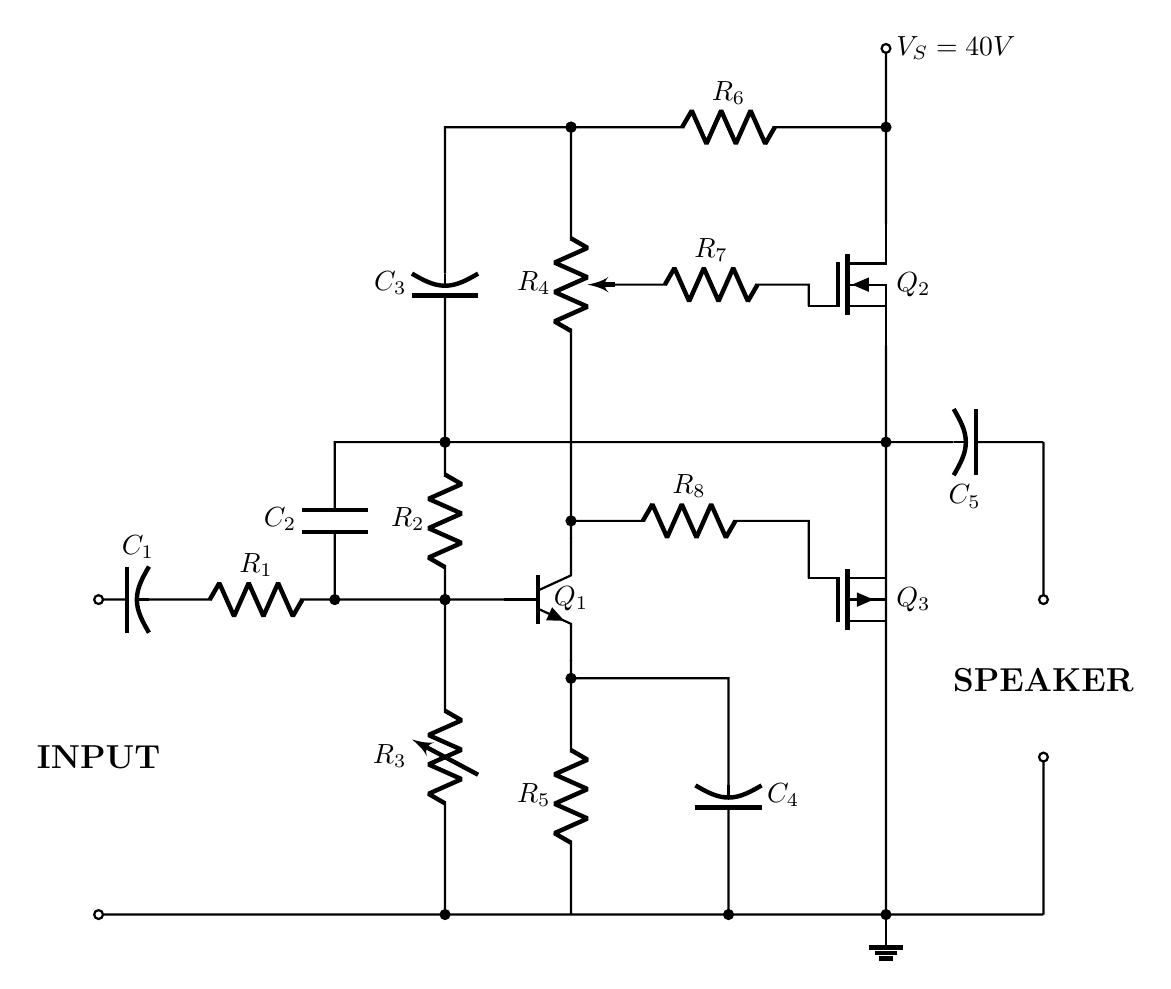
\begin{tikzpicture}[scale=2]
  \draw[color=black, thick]
    (0,0) to [short,o-] (6,0){} % Baseline for connection to ground
    % Input and ground
    (0,1) node[]{\large{\textbf{INPUT}}}
    % Connection of passive components
    (5,0) node[ground]{} node[circ](4.5,0){}
    (0,2) to [cC, l=$C_1$, o-] (0.5,2)
    to [R,l=$R_1$,](1.5,2)
    to node[short]{}(2.6,2)
    (1.5,2) to [C, l=$C_2$, *-] (1.5,3) -| (5,3)
    (2.2,2) to [R, l=$R_2$, *-*] (2.2,3)
    (2.2,3) to [cC, l=$C_3$, *-] (2.2,5) -| (3,5)
    % Transistor Bipolar Q1
    (3,0) to [R,l=$R_5$,-*] (3,1.5)
    to [Tnpn,n=npn1] (3,2.5)
    (npn1.E) node[right=3mm, above=5mm]{$Q_1$} % Labelling the NPN transistor
    (4,0) to [cC, l_=$C_4$, *-] (4, 1.5)--(3,1.5)
    (2.2,0) to [vR, l=$R_3$, *-*] (2.2,2)
    (3,2.5) to node[short]{}(3,3)
    (3,5) to [pR, n=pot1, l_=$R_4$, *-] (3,3)
    (3,5) to [R, l=$R_6$, *-] (5,5)
    to [short,*-o](5,5.5) node[right]{$V_S=40 V$}
    % Mosfet Transistors
    (5,3) to [Tnigfetd,n=mos1] (5,5)
    (mos1.B) node[anchor=west]{$Q_2$} % Labelling MOSFET Q2 Transistor
    (pot1.wiper) to [R, l=$R_7$] (4.5,4) -| (mos1.G)
    (5,1.5) to [Tpigfetd,n=mos2] (5,2.5)
    (5,0) to (mos2.S)
    (3,2.5) to [R, l=$R_8$, *-] (4.5,2.5)
    -| (mos2.G)
    (mos2.B) node[anchor=west]{$Q_3$} % Labelling MOSFET Q3 Transistor
    % Output
    (6,3) to [cC, l=$C_5$,-*](5,3)
    (6,3) to [short,-o] (6,2){}
    (mos1.S)--(mos2.D)
    (6,0) to [short,-o] (6,1){} node[above=7mm]{\large{\textbf{SPEAKER}}}
    ;
\end{tikzpicture}
\end{VerbatimOut}

\MyIO


\begin{VerbatimOut}{z.out}


\section{Kalman Filter System Model}

This Kalman filter system model was done by Burkart Lingner
\cite{lingner2010}.
\ix{Lingner, Burkart}

% An example using TikZ/PGF 2.00
%
% Features: Decorations, Fit, Layers, Matrices, Styles
% Tags: Block diagrams, Diagrams
% Technical area: Electrical engineering

%%%% \documentclass[a4paper,10pt]{article}
%%%% 
%%%% \usepackage[english]{babel}
%%%% \usepackage[T1]{fontenc}
%%%% \usepackage[ansinew]{inputenc}
%%%% 
%%%% \usepackage{lmodern}	% font definition
%%%% \usepackage{amsmath}	% math fonts
%%%% \usepackage{amsthm}
%%%% \usepackage{amsfonts}
%%%% 
%%%% \usepackage{tikz}
%%%% 
%%%% %%%<
%%%% \usepackage{verbatim}
%%%% \usepackage[active,tightpage]{preview}
%%%% \PreviewEnvironment{tikzpicture}
%%%% \setlength\PreviewBorder{5pt}%
%%%% %%%>
%%%% 
%%%% \begin{comment}
%%%% :Title: Kalman Filter System Model
%%%% :Slug: kalman-filter
%%%% :Author: Burkart Lingner
%%%% 
%%%% This is the system model of the (linear) Kalman filter. 
%%%% 
%%%% \end{comment}
%%%% 
%%%% 

\begin{figure}[htbp]
\caption{Kalman filter system model}
\centering
% The state vector is represented by a blue circle.
% "minimum size" makes sure all circles have the same size
% independently of their contents.
\tikzstyle{state}=[circle,
                                    thick,
                                    minimum size=1.2cm,
                                    draw=blue!80,
                                    fill=blue!20]

% The measurement vector is represented by an orange circle.
\tikzstyle{measurement}=[circle,
                                                thick,
                                                minimum size=1.2cm,
                                                draw=orange!80,
                                                fill=orange!25]

% The control input vector is represented by a purple circle.
\tikzstyle{input}=[circle,
                                    thick,
                                    minimum size=1.2cm,
                                    draw=purple!80,
                                    fill=purple!20]

% The input, state transition, and measurement matrices
% are represented by gray squares.
% They have a smaller minimal size for aesthetic reasons.
\tikzstyle{matrx}=[rectangle,
                                    thick,
                                    minimum size=1cm,
                                    draw=gray!80,
                                    fill=gray!20]

% The system and measurement noise are represented by yellow
% circles with a "noisy" uneven circumference.
% This requires the TikZ library "decorations.pathmorphing".
\tikzstyle{noise}=[circle,
                                    thick,
                                    minimum size=1.2cm,
                                    draw=yellow!85!black,
                                    fill=yellow!40,
                                    decorate,
                                    decoration={random steps,
                                                            segment length=2pt,
                                                            amplitude=2pt}]

% Everything is drawn on underlying gray rectangles with
% rounded corners.
\tikzstyle{background}=[rectangle,
                                                fill=gray!10,
                                                inner sep=0.2cm,
                                                rounded corners=5mm]

\begin{tikzpicture}[>=latex,text height=1.5ex,text depth=0.25ex]
    % "text height" and "text depth" are required to vertically
    % align the labels with and without indices.
  
  % The various elements are conveniently placed using a matrix:
  \matrix[row sep=0.5cm,column sep=0.5cm] {
    % First line: Control input
    &
        \node (u_k-1) [input]{$\mathbf{u}_{k-1}$}; &
        &
        \node (u_k)   [input]{$\mathbf{u}_k$};     &
        &
        \node (u_k+1) [input]{$\mathbf{u}_{k+1}$}; &
        \\
        % Second line: System noise & input matrix
        \node (w_k-1) [noise] {$\mathbf{w}_{k-1}$}; &
        \node (B_k-1) [matrx] {$\mathbf{B}$};       &
        \node (w_k)   [noise] {$\mathbf{w}_k$};     &
        \node (B_k)   [matrx] {$\mathbf{B}$};       &
        \node (w_k+1) [noise] {$\mathbf{w}_{k+1}$}; &
        \node (B_k+1) [matrx] {$\mathbf{B}$};       &
        \\
        % Third line: State & state transition matrix
        \node (A_k-2)         {$\cdots$};           &
        \node (x_k-1) [state] {$\mathbf{x}_{k-1}$}; &
        \node (A_k-1) [matrx] {$\mathbf{A}$};       &
        \node (x_k)   [state] {$\mathbf{x}_k$};     &
        \node (A_k)   [matrx] {$\mathbf{A}$};       &
        \node (x_k+1) [state] {$\mathbf{x}_{k+1}$}; &
        \node (A_k+1)         {$\cdots$};           \\
        % Fourth line: Measurement noise & measurement matrix
        \node (v_k-1) [noise] {$\mathbf{v}_{k-1}$}; &
        \node (H_k-1) [matrx] {$\mathbf{H}$};       &
        \node (v_k)   [noise] {$\mathbf{v}_k$};     &
        \node (H_k)   [matrx] {$\mathbf{H}$};       &
        \node (v_k+1) [noise] {$\mathbf{v}_{k+1}$}; &
        \node (H_k+1) [matrx] {$\mathbf{H}$};       &
        \\
        % Fifth line: Measurement
        &
        \node (z_k-1) [measurement] {$\mathbf{z}_{k-1}$}; &
        &
        \node (z_k)   [measurement] {$\mathbf{z}_k$};     &
        &
        \node (z_k+1) [measurement] {$\mathbf{z}_{k+1}$}; &
        \\
    };
    
    % The diagram elements are now connected through arrows:
    \path[->]
        (A_k-2) edge[thick] (x_k-1)	% The main path between the
        (x_k-1) edge[thick] (A_k-1)	% states via the state
        (A_k-1) edge[thick] (x_k)		% transition matrices is
        (x_k)   edge[thick] (A_k)		% accentuated.
        (A_k)   edge[thick] (x_k+1)	% x -> A -> x -> A -> ...
        (x_k+1) edge[thick] (A_k+1)
        
        (x_k-1) edge (H_k-1)				% Output path x -> H -> z
        (H_k-1) edge (z_k-1)
        (x_k)   edge (H_k)
        (H_k)   edge (z_k)
        (x_k+1) edge (H_k+1)
        (H_k+1) edge (z_k+1)
        
        (v_k-1) edge (z_k-1)				% Output noise v -> z
        (v_k)   edge (z_k)
        (v_k+1) edge (z_k+1)
        
        (w_k-1) edge (x_k-1)				% System noise w -> x
        (w_k)   edge (x_k)
        (w_k+1) edge (x_k+1)
        
        (u_k-1) edge (B_k-1)				% Input path u -> B -> x
        (B_k-1) edge (x_k-1)
        (u_k)   edge (B_k)
        (B_k)   edge (x_k)
        (u_k+1) edge (B_k+1)
        (B_k+1) edge (x_k+1)
        ;
    
    % Now that the diagram has been drawn, background rectangles
    % can be fitted to its elements. This requires the TikZ
    % libraries "fit" and "background".
    % Control input and measurement are labeled. These labels have
    % not been translated to English as "Measurement" instead of
    % "Messung" would not look good due to it being too long a word.
    \begin{pgfonlayer}{background}
        \node [background,
                    fit=(u_k-1) (u_k+1),
                    label=left:Entrance:] {};
        \node [background,
                    fit=(w_k-1) (v_k-1) (A_k+1)] {};
        \node [background,
                    fit=(z_k-1) (z_k+1),
                    label=left:Measure:] {};
    \end{pgfonlayer}
\end{tikzpicture}

\end{figure}
\end{VerbatimOut}

\MyIO


  % Linguistics.
  %\ProvidesFile{ap-linguistics.tex}[2022-10-05 linguistics appendix]

\begin{VerbatimOut}{z.out}
\chapter{LINGUISTICS}
\ix{linguistics//Linguistics appendix}

See WIKIBOOKS \LaTeX/Linguistics \cite{wikibooks-latex-linguistics}
or google for the information you need.

The doulossil font
\cite{tambe2020}
is a TrueType font.
Version 0.1 on September 21, 2020 claimed
``it has characters that are not in other TeX IPA fonts''.
\end{VerbatimOut}

\MyIO


\begin{VerbatimOut}{z.out}


\section{Demonstrate the example and examples environments}

The example and examples environment
are defined
in the covington
\cite{covington2021}
package.

Demonstrate the example environment:
\begin{example}
  This is an example.
  This is an example.
\end{example}

Demonstrate the examples environment:
\begin{examples}
  \item First example.
  \item Second example.
\end{examples}
\end{VerbatimOut}

\MyIO


  % Mathematics.
  %\ProvidesFile{ap-mathematics.tex}[2022-10-05 mathematics appendix]

\begin{VerbatimOut}{z.out}
\chapter{MATHEMATICS}
\ix{mathematics//Mathematics appendix}

\PurdueThesisLogo\ loads the \AMSmathLogo\ package
\cite{amslatex3project2019}
to do mathematics.
\end{VerbatimOut}


\subsection{Photoswitching induced spatial coherence}

Photoswitching fluorescent molecules are described in the density matrix formalism

\begin{equation*}
\rho = \xi\ket{\alpha}\bra{\alpha} + (1-\xi)\ket{0}\bra{0}
\end{equation*}

where $\ket{\alpha}$ is a coherent state with amplitude $\alpha$ i.e., $\langle n\rangle = \bra{\alpha} n\ket{\alpha} = |\alpha|^{2}$. We consider a simplified model consisting of a single mode field 

\begin{equation*}
E_{0}^{+}\sim \sum_{j=1}^{M}\delta(s-s_{j})a_{j} \;\; E^{+}(r_{i}) = \int d^{2}s E_{0}^{+} h(r-s) = h(r_{i}-s)\hat{a}
\end{equation*}

\begin{equation*}
g^{(2)}_{ij}(0) = \frac{\langle E^{-}(r_{i})E^{-}(r_{j})E^{+}(r_{i})E^{+}(r_{j}) \rangle}{\langle E^{-}(r_{i})E^{+}(r_{i})\rangle\langle E^{-}(r_{j})E^{+}(r_{j})\rangle} = \frac{\mathrm{Tr}(a^{\dagger}a^{\dagger}aa\rho)}{\mathrm{Tr}(a^{\dagger}a\rho)^{2}}
\end{equation*}

Notice that terms related to point spread function will cancel. Now,

\begin{align*}
\mathrm{Tr}(a^{\dagger}a^{\dagger}aa\rho) &= \mathrm{Tr}(a^{\dagger}a^{\dagger}aa \left(\xi\ket{\alpha}\bra{\alpha} + (1-\xi)\ket{0}\bra{0}\right))\\
&= \mathrm{Tr}\left(\xi e^{-|\alpha|^{2}}\sum_{n,m}^{\infty}\frac{\alpha^{n}}{n!}\ket{n}\bra{m}\right)\\
&= \mathrm{Tr}\left(\xi e^{-|\alpha|^{2}}\sum_{n}^{\infty}\frac{|\alpha|^{2n}}{n!}n(n-1)\right)\\
&= \mathrm{Tr}\left(\xi e^{-|\alpha|^{2}}\sum_{n=2}^{\infty}\frac{|\alpha|^{2n}}{(n-2)!}\right)\\
&= \xi|\alpha|^{4}
\end{align*}

The second trace in the denominator proceeds similarly to the first

\begin{align*}
\mathrm{Tr}(a^{\dagger}a\rho) &= \mathrm{Tr}(a^{\dagger}a \left(\xi\ket{\alpha}\bra{\alpha} + (1-\xi)\ket{0}\bra{0}\right))\\
&= \mathrm{Tr}\left(\xi e^{-|\alpha|^{2}}\sum_{n,m}^{\infty}\frac{\alpha^{n}}{n!}\ket{n}\bra{m} \right)\\
&= \mathrm{Tr}\left(\xi e^{-|\alpha|^{2}}\sum_{n}^{\infty}\frac{|\alpha|^{2n}}{n!}n\right)\\
&= \mathrm{Tr}\left(\xi e^{-|\alpha|^{2}}\sum_{n=2}^{\infty}\frac{|\alpha|^{2n}}{(n-1)!}\right)\\
&= \xi|\alpha|^{2}
\end{align*}

As expected, this gives $\langle n\rangle$. Putting it all together yields a simple expression for the two-point coherence function

\begin{equation*}
g^{(2)}_{ij}(0) = \frac{\xi|\alpha|^{4}}{\xi^{2}|\alpha|^{4}} = \frac{1}{\xi}
\end{equation*}

Notice that as $\xi\rightarrow 1$ (always on) we recover the coherent state. As $\xi\rightarrow 0$ we observe $g^{(2)}_{ij}(0) > 1$ i.e., bunching. This is a critical result: photoswitching results in non-trivial correlations between pixels $i$ and $j$. Introducing more than one photoswitching emitter gives? In practice, we can estimate of $g^{(2)}_{ij}(0)$ in a finite time interval. I guess that $\langle n_{i}\rangle = \xi |\alpha|^{2}\Delta = 0.5$ is reasonable; however this is best addressed by Monte Carlo simulation. The total interval $T$ constrained by the super-resolution frame rate e.g., $T=10\mathrm{ms}$. 



\subsection{Details of the Gaussian PSF}

We will derive the gradients for the integrated astigmatic Gaussian, since it is the more general case. As before, define $i_{0} = g_{k}\gamma\Delta t N_{0}$ such that $\mu_{k}' = i_{0}\lambda_{k}$

\begin{equation*}
J_{x_{0}} = \beta_{k}\lambda_{y}\frac{\partial \lambda_{x}}{\partial x_{0}} \;\; J_{y_{0}} = \beta_{k}\lambda_{x}\frac{\partial \lambda_{y}}{\partial y_{0}}\;\;\; J_{z_{0}}  = \frac{\partial \mu_{k}'}{\partial \sigma_{x}}\frac{\partial \sigma_{x}}{\partial z_{0}} + \frac{\partial \mu_{k}'}{\partial \sigma_{y}}\frac{\partial \sigma_{y}}{\partial z_{0}}
\end{equation*}

\begin{align*}
J_{x_{0}} &= \beta_{k}\lambda_{y}\frac{\partial \lambda_{x}}{\partial x_{0}} \\
&= \frac{\beta_{k}\lambda_{y}}{2}\frac{\partial}{\partial x_{0}}\left(\mathrm{erf}\left(\frac{x_{k}+\frac{1}{2}-x_{0}}{\sqrt{2}\sigma_{x}}\right) -\mathrm{erf}\left(\frac{x_{k}-\frac{1}{2}-x_{0}}{\sqrt{2}\sigma_{x}}\right)\right)\\
&= \frac{\beta_{k}\lambda_{y}}{\sqrt{2\pi}\sigma_{x}}\left(\mathrm{exp}\left(\frac{(x_{k}-\frac{1}{2}-x_{0})^{2}}{2\sigma_{x}^{2}}\right) -\mathrm{exp}\left(\frac{(x_{k}+\frac{1}{2}-x_{0})^{2}}{2\sigma_{x}^{2}}\right)\right)
\end{align*}

\begin{align*}
J_{y_{0}} &= \beta_{k}\lambda_{x}\frac{\partial \lambda_{y}}{\partial y_{0}} \\
&= \frac{\beta_{k}\lambda_{x}}{2}\frac{\partial}{\partial y_{0}}\left(\mathrm{erf}\left(\frac{y_{k}+\frac{1}{2}-y_{0}}{\sqrt{2}\sigma_{y}}\right) -\mathrm{erf}\left(\frac{y_{k}-\frac{1}{2}-y_{0}}{\sqrt{2}\sigma_{y}}\right)\right)\\
&= \frac{\beta_{k}\lambda_{x}}{\sqrt{2\pi}\sigma_{y}}\left(\mathrm{exp}\left(\frac{(y_{k}-\frac{1}{2}-y_{0})^{2}}{2\sigma_{y}^{2}}\right) -\mathrm{exp}\left(\frac{(y_{k}+\frac{1}{2}-y_{0})^{2}}{2\sigma_{y}^{2}}\right)\right)
\end{align*}

\begin{align*}
J_{\sigma_{x}} &= \beta_{k}\lambda_{y}\frac{\partial \lambda_{x}}{\partial \sigma_{x}} \\
&= \frac{\beta_{k}\lambda_{y}}{2}\frac{\partial}{\partial \sigma_{x}}\left(\mathrm{erf}\left(\frac{x_{k}+\frac{1}{2}-x_{0}}{\sqrt{2}\sigma_{x}}\right) -\mathrm{erf}\left(\frac{x_{k}-\frac{1}{2}-x_{0}}{\sqrt{2}\sigma_{x}}\right)\right)\\
&= \frac{\beta_{k}\lambda_{y}}{\sqrt{2\pi}}\left(\frac{\left(x-x_{0}-\frac{1}{2}\right) e^{-\frac{\left(x-x_{0}-\frac{1}{2}\right)^2}{2 \sigma_{x} ^2}}}{\sigma_{x} ^2}-\frac{ \left(x-x_{0}+\frac{1}{2}\right) e^{-\frac{\left(x-x_{0}+\frac{1}{2}\right)^2}{2 \sigma_{x} ^2}}}{\sigma_{x} ^2}\right)
\end{align*}

\begin{align*}
J_{\sigma_{y}} &= \beta_{k}\lambda_{x}\frac{\partial \lambda_{y}}{\partial \sigma_{y}} \\
&= \frac{\beta_{k}\lambda_{x}}{2}\frac{\partial}{\partial \sigma_{y}}\left(\mathrm{erf}\left(\frac{y_{k}+\frac{1}{2}-y_{0}}{\sqrt{2}\sigma_{y}}\right) -\mathrm{erf}\left(\frac{y_{k}-\frac{1}{2}-y_{0}}{\sqrt{2}\sigma_{y}}\right)\right)\\
&= \frac{\beta_{k}\lambda_{x}}{\sqrt{2\pi}}\left(\frac{\left(y-y_{0}-\frac{1}{2}\right) e^{-\frac{\left(y-y_{0}-\frac{1}{2}\right)^2}{2 \sigma_{y} ^2}}}{\sigma_{y} ^2}-\frac{ \left(y-y_{0}+\frac{1}{2}\right) e^{-\frac{\left(y-y_{0}+\frac{1}{2}\right)^2}{2 \sigma_{y} ^2}}}{\sigma_{y} ^2}\right)
\end{align*}

Luckily, computing the Hessian matrix for (2.9) is tractable, and is actually quite simple when one takes advantage of the chain rule for Hessian matrices. Looking at (2.9), the likelihood is a hierarchical function that maps a vector space $\Theta$ to a vector space $\Lambda$ to a scalar value. Formally, we define $T: \Theta \rightarrow \Lambda$ and $W: \Lambda \rightarrow \mathbb{R}$. The parameter vector $(x_{0},y_{0},z_{0}, \sigma_{0}, N_{0})\in \Theta$, the Poisson rate vector $\vec{\lambda} \in \Lambda$ and $\ell \in \mathbb{R}$. Note that we choose to optimize $\sigma_{x}$ and $\sigma_{y}$ directly and compute $z_{0}$ to simplify the computation of the Hessian. To get the Hessian, we need the chain-rule for Hessian matrices, which can be quickly computed in terms of the jacobian and hessian of $T$ and $W$.


\begin{equation*}
H_{\ell} = J_{\mu}^{T} H_{\ell} J_{\mu} + (J_{\ell}\otimes I_{n})H_{\mu}
\end{equation*}

where we have used $J_{\mu}$ to represent the jacobian of $T$ and $J_{\ell}$ for the jacobian of $W$. Similar notation is used for the corresponding Hessian matrices. 
In the 3D case, the Hessian matrix is not directly separable since $\mu \propto \lambda_{x}(x_{0},\sigma_{0},\sigma_{x})\lambda_{y}(y_{0},\sigma_{0},\sigma_{y})$. To see this, an abstract representation of the Hessian reads 


\subsection{Fisher information for 2D integrated gaussian}

For the 2D integrated gaussian point spread function, the Hessian only contains separable second order derivatives, so the Fisher information matrix takes on a convenient form

\begin{equation}
I_{ij}(\theta) = \underset{\theta}{\mathbb{E}}\left(\frac{\partial \ell}{\partial\theta_{i}}\frac{\partial\ell}{\partial\theta_{j}}\right) 
\end{equation}

For an arbitrary parameter then we have

\begin{align*}
\frac{\partial \ell}{\partial \theta_{i}} &= \frac{\partial}{\partial \theta_{i}} \sum_{k}  x_{k}\log x_{k} + \mu_{k}' - x_{k}\log\left(\mu_{k}'\right)\\
&= \sum_{k} \frac{\partial \mu_{k}'}{\partial\theta_{i}} \left(\frac{\mu_{k}'-x_{k}}{\mu_{k}'}\right)
\end{align*}

\begin{equation*}
I_{ij}(\theta) = \underset{\theta}{\mathbb{E}}\left(\sum_{k}\frac{\partial \mu_{k}'}{\partial\theta_{i}}\frac{\partial \mu_{k}'}{\partial\theta_{j}} \left(\frac{\mu_{k}'-x_{k}}{\mu_{k}'}\right)^{2}\right) = \sum_{k}\frac{1}{\mu_{k}'}\frac{\partial \mu_{k}'}{\partial\theta_{i}}\frac{\partial \mu_{k}'}{\partial\theta_{j}}
\end{equation*}

To compute the bound, it turns out all we need is the jacobian $\frac{\partial \mu_{k}'}{\partial\theta_{j}} $.

\section{The Fokker-Planck Equation}

The Fokker-Planck equation is a central tool in non-equilibrium statistical mechanics, analagous to the master equation for discrete systems. It allows us to determine the time evolution of probability densities over continuous state spaces. Important examples in biophysics are the phase space of a particle or the membrane potential of a nerve cell.

Suppose we have a random variable $\bm{x}$ and its joint distribution $P(\bm{x},t)$, which is not necessarily stationary. Define a vector field $\vec{J}(\bm{x},t)$ which is the probability current, which we will specify in a moment. The Fokker-Planck equation is by starting with a continuity equation for probability 

\begin{align*}
\frac{d}{dt}\int_{V_{0}} P(\bm{x},t)dV &= \int_{S}P(\bm{x},t)(\vec{J}\cdot\hat{n})dS\\
&= -\int_{V_{0}}P(\bm{x},t)(\nabla\cdot \vec{J})dV
\end{align*}

Clearly this implies that

\begin{equation*}
\frac{dP(\bm{x},t)}{dt} = -\left(\nabla\cdot \vec{J}\right)P(\bm{x},t)
\end{equation*}

We often call the divergence term, the Fokker-Planck operator $\mathcal{L}_{FP}=-\nabla\cdot \vec{J}$. A more rigorous derivation is given in the appendix, which tells us that, to second order

\begin{equation*}
J(x_{i},t)  = \left(M_{i}^{(1)}(t) - \sum_{j}\frac{\partial}{\partial x_{j}}M_{ij}^{(2)}(t) \right)P(\bm{x},t)
\end{equation*}

where $M_{i}^{n}(t)$ is the $n$th moment of a transition kernel $T(x_{i}',t'|x_{i},t)$ for variable $i$. The first moment is essentially just the deterministic part of the Langevin dynamics. The second and higher moments will depend on these higher moments in the stochastic forcing terms. As proven more completely in the appendix, the full multi-dimensional Fokker-Planck equation reads

\begin{align}
\frac{\partial P(\vec{x},t)}{\partial t}  &= \vec{\nabla} \cdot J(\vec{x},t)\\
&= \sum_{i=1}^{N}\left(-\frac{\partial}{\partial x_{i}}M_{i}^{(1)}(t) + \sum_{j=1}^{N} \frac{\partial^{2}}{\partial x_{i}\partial x_{j}}M_{ij}^{(2)}(t)\right)P(\vec{x},t)
\end{align}

If we make a further constraint that the moments of the transition operator are stationary $M_{i}^{(1)}(t) = \Upsilon_{ij}$ and $M_{ij}^{(2)}(t) = D_{ij}$ 

\begin{align}
\frac{\partial P(\vec{x},t)}{\partial t}  &= \sum_{ij}\left(\Upsilon_{ij}\frac{\partial}{\partial x_{i}} + D_{ij}\frac{\partial^{2}}{\partial x_{i}\partial x_{j}}\right)P(\vec{x},t)
\end{align}

\begin{equation*}
D = \begin{pmatrix}0&0 \\ 0& \gamma k_{B}T/m \end{pmatrix}\;\;\Upsilon = \begin{pmatrix}0 & -1\\ 0 & \gamma\end{pmatrix}
\end{equation*}

\section{Free Brownian particle}

Consider a familiar Langevin dynamics on phase space $\bm{x} = (x,v)$, where a free particle ($V(x)=0\; \forall x$) experiences a viscous drag force and stochastic forcing $\xi(t)$ where $\xi(t)\sim\mathcal{N}(\mu,\sigma^{2})$ and $\langle \xi(t)\xi(t+\tau)\rangle = \delta(t-\tau)$. 

\begin{align*}
\dot{x} &= v\\
\dot{v} &= -\frac{\gamma}{m}v + \frac{1}{m}\xi(t)
\end{align*}

The moments of the transition kernel must be

\begin{equation*}
M_{x}^{(1)} = v  \;\; M_{v}^{(1)} = -\frac{\gamma}{m}v + \mu \;\; M_{v}^{(v)} = \sigma^{2}
\end{equation*}

To simplify the notation let us define $\nabla\cdot \vec{J} = \frac{\partial J_{x}}{\partial x} + \frac{\partial J_{x}}{\partial v}= \mathcal{L}_{x} + \mathcal{L}_{v} = \mathcal{L}_{FP}$. This gives the full Fokker-Planck equation $\frac{dP(\bm{x},t)}{dt} = -\mathcal{L}_{FP}P(\bm{x},t)$. 

\begin{align*}
\mathcal{L}_{x}P(\bm{x},t) &= \frac{\partial}{\partial x}\left(vP(\bm{x},t)\right)\\
\mathcal{L}_{v}P(\bm{x},t) &= \frac{\partial}{\partial v}\left(-\frac{\gamma}{m}v + \frac{1}{m}F(x)\right)P(\bm{x},t) + \sigma^{2}\frac{\partial^{2}}{\partial v^{2}}P(\bm{x},t)
\end{align*}


\section{The Brownian Harmonic oscillator}

Consider a familiar Langevin dynamics on phase space $\bm{x} = (x,v)$, where a particle in a potential $V(x)$ experiences a viscous drag force and stochastic forcing $\xi(t)$ where $\xi(t)\sim\mathcal{N}(\mu,\sigma^{2})$ and $\langle \xi(t)\xi(t+\tau)\rangle = \delta(t-\tau)$. 

\begin{align*}
\dot{x} &= v\\
\dot{v} &= -\frac{\gamma}{m}v + \frac{1}{m}F(x) + \frac{1}{m}\xi(t)
\end{align*}

The moments of the transition kernel must be

\begin{equation*}
M_{x}^{(1)} = v  \;\; M_{v}^{(1)} = -\frac{\gamma}{m}v + \frac{1}{m}F(x) + \mu \;\; M_{v}^{(v)} = \sigma^{2}
\end{equation*}

To simplify the notation let us define $\nabla\cdot \vec{J} = \frac{\partial J_{x}}{\partial x} + \frac{\partial J_{x}}{\partial v}= \mathcal{L}_{x} + \mathcal{L}_{v} = \mathcal{L}_{FP}$. This gives the full Fokker-Planck equation $\frac{dP(\bm{x},t)}{dt} = -\mathcal{L}_{FP}P(\bm{x},t)$. 

\begin{align*}
\mathcal{L}_{x}P(\bm{x},t) &= \frac{\partial}{\partial x}\left(vP(\bm{x},t)\right)\\
\mathcal{L}_{v}P(\bm{x},t) &= \frac{\partial}{\partial v}\left(-\frac{\gamma}{m}v + \frac{1}{m}F(x)\right)P(\bm{x},t) + \sigma^{2}\frac{\partial^{2}}{\partial v^{2}}P(\bm{x},t)
\end{align*}


  % Music.
  %\ProvidesFile{ap-music.tex}[2022-10-05 music appendix]

\begin{VerbatimOut}{z.out}
\chapter{MUSIC}
\ix{music//Music appendix}

To get the following printed music score I did the following steps.
\begin{itemize}
  \item
    Get the ``Example of LilyPond input file''
    from the Wikipedia LilyPond page
    \cite{wikipedia-lilypond}
    and put it in a \verb+fib.ly+ file.
  \item
    Ran \verb+lilypond fib.ly+ and got the following \verb+fib.pdf+ file:
\end{itemize}
\ix{LilyPond music typesetting software}

\noindent 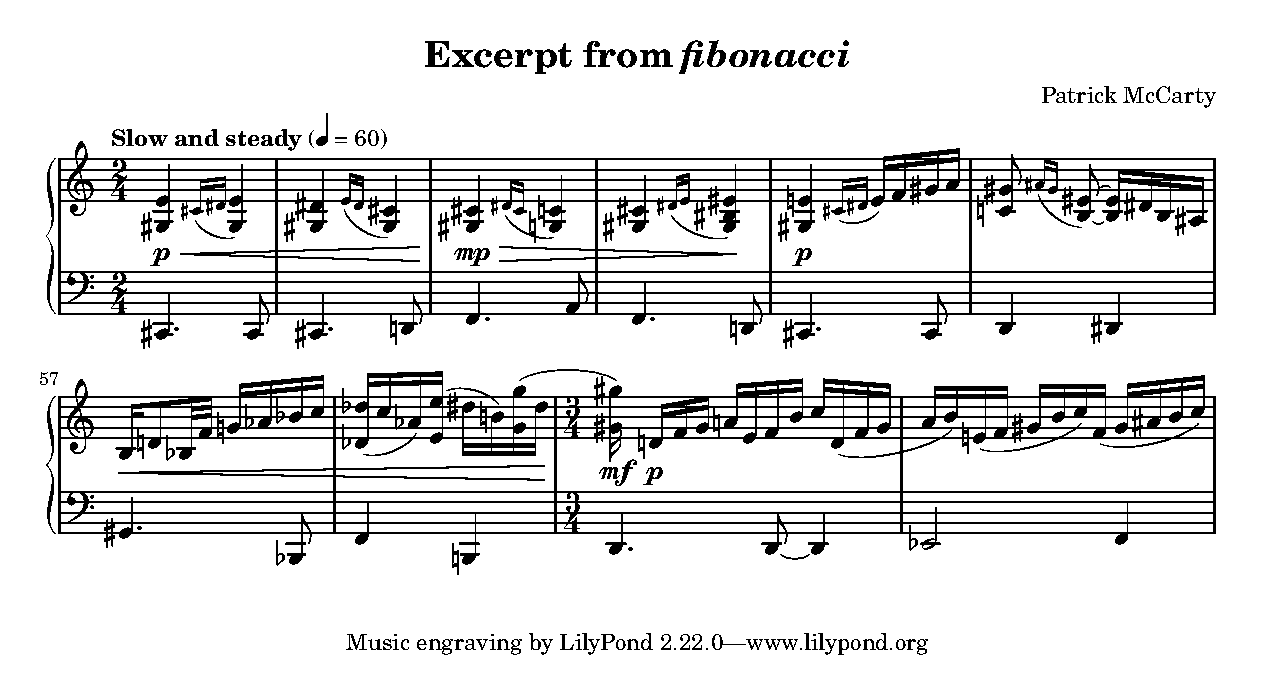
\includegraphics[scale=0.77]{gr-fib.pdf}
\end{VerbatimOut}

\MyIO


  % The examples in ap-physics require LuaLaTeX but LuaLaTeX
  % screws up the spacing in the List of Figures.  So, the
  % ap-physics file is not included.
  %
  % For some reason, ap-physics doesn't work when using BibTeX.
  % Just enclosing \ProvidesFile{ap-physics.tex}[2022-10-05 Physics appendix]

\chapter{Optical fluctuation microscopy}
\ix{physics//Physics appendix}

\subsection{Spatial coherence for an isolated emitter}

Photoswitching fluorescent molecules are described in the density matrix formalism

\begin{equation*}
\rho = \sum_{k}\xi_{k}\ket{\alpha_{k}}\bra{\alpha_{k}}\;\; \sum_{k}\xi_{k} = 1
\end{equation*}


where $\ket{\alpha_{k}}$ is a coherent state with amplitude $\alpha_{k}$ i.e., $\langle n\rangle = \bra{\alpha_{k}} n\ket{\alpha_{k}} = \lvert\alpha_{k}^{2}\rvert$. Typically $\xi_{k}$ and $\langle n_{k}\rangle$ are heterogeneous. We consider a simplified model consisting of a single mode field 

\begin{equation*}
E^{+}(r_{i}) = h(r_{i}-s_{0})\hat{a}_{n}
\end{equation*}

\begin{equation*}
g^{(2)}_{ij}(0) = \frac{\langle E^{-}(r_{i})E^{-}(r_{j})E^{+}(r_{i})E^{+}(r_{j}) \rangle}{\langle E^{-}(r_{i})E^{+}(r_{i})\rangle\langle E^{-}(r_{j})E^{+}(r_{j})\rangle} = \frac{\mathrm{Tr}(E^{-}(r_{i})E^{-}(r_{j})E^{+}(r_{i})E^{+}(r_{j})\rho)}{\mathrm{Tr}(E^{-}(r_{i})E^{+}(r_{i})\rho)\mathrm{Tr}(E^{-}(r_{j})E^{+}(r_{j})\rho)}
\end{equation*}

Terms related to point spread function will cancel. It is instructive to compute

\begin{align*}
\mathrm{Tr}(a^{\dagger}a^{\dagger}aa \left(\xi_{k}\ket{\alpha_{k}}\bra{\alpha_{k}}\right) &= \mathrm{Tr}\left(\xi_{k} e^{-\lvert\alpha\rvert^{2}}\sum_{n,m}^{\infty}\frac{\alpha^{n}}{n!}\ket{n}\bra{m}\right)\\
&= \mathrm{Tr}\left(\xi_{k} e^{-\lvert\alpha\rvert^{2}}\sum_{n}^{\infty}\frac{\lvert\alpha\rvert^{2n}}{n!}n(n-1)\right)\\
&= \mathrm{Tr}\left(\xi_{k} e^{-\lvert\alpha\rvert^{2}}\sum_{n=2}^{\infty}\frac{\lvert\alpha\rvert^{2n}}{(n-2)!}\right)\\
&= \xi_{k}\lvert\alpha_{k}\rvert^{4}
\end{align*}

Similarly,

\begin{align*}
\mathrm{Tr}(a^{\dagger}a \left(\xi \ket{\alpha}\bra{\alpha}\right)) &= \mathrm{Tr}\left(\xi e^{-\lvert\alpha\rvert^{2}}\sum_{n,m}^{\infty}\frac{\alpha^{n}(\alpha^{m})^{*}}{\sqrt{n!}\sqrt{m!}}a^{\dagger}a\ket{n}\bra{m} \right)\\
&= \xi e^{-\lvert\alpha\rvert^{2}}\sum_{n=0}^{\infty}\frac{(\lvert\alpha\rvert^{2})^{n}}{n!}n\\
&= \xi e^{-\lvert\alpha\rvert^{2}}\sum_{n=1}^{\infty}\frac{(\lvert\alpha\rvert^{2})^{n}}{(n-1)!}\\
&= \xi e^{-\lvert\alpha\rvert^{2}}\left(\lvert\alpha\rvert^{2} + \frac{\lvert\alpha\rvert^{4}}{1!} + \frac{\lvert\alpha\rvert^{6}}{2!}+...\right)\\
&= \xi e^{-\lvert\alpha\rvert^{2}}\lvert\alpha\rvert^{2}\left(1 + \frac{\lvert\alpha\rvert^{2}}{1!} + \frac{\lvert\alpha\rvert^{3}}{2!}+...\right)\\
&= \xi e^{-\lvert\alpha\rvert^{2}}e^{\lvert\alpha\rvert^{2}}\lvert\alpha\rvert^{2} = \xi\lvert\alpha\rvert^{2}
\end{align*}

\begin{align*}
\mathrm{Tr}(a a^{\dagger} \left(\xi \ket{\alpha}\bra{\alpha}\right)) &= \mathrm{Tr}\left(\xi e^{-\lvert\alpha\rvert^{2}}\sum_{n,m}^{\infty}\frac{\alpha^{n}(\alpha^{m})^{*}}{\sqrt{n!}\sqrt{m!}}a a^{\dagger}\ket{n}\bra{m} \right)\\
&= \xi e^{-\lvert\alpha\rvert^{2}}\sum_{n=0}^{\infty}\frac{(\lvert\alpha\rvert^{2})^{n}}{n!}(n+1)\\
&= \xi e^{-\lvert\alpha\rvert^{2}}\left(\sum_{n=1}^{\infty}\frac{(\lvert\alpha\rvert^{2})^{n}}{(n-1)!} + e^{\lvert\alpha\rvert^{2}}\right)\\
&= \xi e^{-\lvert\alpha\rvert^{2}}\left(\lvert\alpha\rvert^{2}e^{\lvert\alpha\rvert^{2}} + e^{\lvert\alpha\rvert^{2}}\right) = \xi(\lvert\alpha\rvert^{2} + 1)
\end{align*}

Putting it all together yields a simple expression for the two-point coherence function

\begin{equation*}
g^{(2)}_{ij}(0) = \frac{\sum_{k}\xi_{k}\lvert\alpha_{k}\rvert^{4}}{\left(\sum_{k}\xi_{k}\lvert\alpha_{k}\rvert^{2}\right)\left(\sum_{k}\xi_{k}\lvert\alpha_{k}\rvert^{2}\right)}
\end{equation*}

For example, if we have a two-level system consisting of a fluorescent state with amplitude $\alpha$ and the vacuum state, this becomes

\begin{equation*}
g^{(2)}_{ij}(0) = \frac{\xi\lvert\alpha\rvert^{4}}{\xi^{2}\lvert\alpha\rvert^{4}} = \frac{1}{\xi}
\end{equation*}

As $\xi\rightarrow 1$ (always on) we recover a coherent state. As $\xi\rightarrow 0$ we observe $g^{(2)}_{ij}(0) > 1$ i.e., bunching.

\subsection{Generalization to nonzero background}

\begin{equation*}
E_{0}^{+}\sim \sum_{j=1}^{M}\delta(s-s_{j})a_{j} \;\; E^{+}(r_{i}) = \int d^{2}s E_{0}^{+} = \sum_{n}h(r_{i}-s_{n})a_{n}
\end{equation*}

\begin{equation*}
\rho_{S} = \xi\ket{\alpha}\bra{\alpha} + (1-\xi)\ket{0}\bra{0}\;\;\rho_{B} = \ket{\beta}\bra{\beta}\;\;\rho = \rho_{S}\otimes\rho_{B}
\end{equation*}

\begin{equation*}
E(r_{i})^{+} = E_{S}(r_{i})^{+} + E_{B}(r_{i})^{+} = h(r_{i}-s_{n})a_{S} + a_{B}
\end{equation*}

\begin{align*}
G^{2}_{ij}(0) &= \langle(E_{S}^{\dagger} + E_{B}^{\dagger}) (E_{S}^{\dagger} + E_{B}^{\dagger})( E_{S} + E_{B}) (E_{S} + E_{B})\rangle \\
&= h_{i}^{2}h_{j}^{2}\langle a_{S}^{\dagger}a_{S}^{\dagger}a_{S}a_{S}\rangle + h_{i}^{2}\langle a_{S}^{\dagger}a_{B}^{\dagger}a_{S}a_{B}\rangle + h_{j}^{2}\langle a_{B}^{\dagger}a_{S}^{\dagger}a_{B}a_{S}\rangle  + \langle a_{B}^{\dagger}a_{B}^{\dagger}a_{B}a_{B}\rangle  \\
&= \xi(h_{i}^{2}h_{j}^{2}\lvert\alpha\rvert^{4}+ h_{i}^{2}\lvert\alpha\rvert^{2}\lvert\beta\rvert^{2} + h_{j}^{2}\lvert\alpha\rvert^{2}\lvert\beta\rvert^{2}\rangle  + \lvert\beta\rvert^{4} ) \\
&= \xi(h_{i}^{2}h_{j}^{2}\lvert\alpha\rvert^{4}+ \lvert\alpha\rvert^{2}\lvert\beta\rvert^{2}(h_{i}^{2} + h_{j}^{2})  + \lvert\beta\rvert^{4}) \\
\end{align*}

The normalized second order coherence function then reads

\begin{align*}
g^{2}_{ij}(0) &= \frac{\xi h_{i}^{2}h_{j}^{2}N_{0}^{2} + \xi N_{0}B_{0}(h_{i}^{2} + h_{j}^{2}) + B_{0}^{2}}{\xi^{2} h_{i}^{2}h_{j}^{2}N_{0}^{2} + \xi N_{0}B_{0}(h_{i}^{2}+h_{j}^{2}) +  B_{0}^{2}}
\end{align*}

Notice the PSF factor $h_{i}$ appears squared. This squared value can be seen as the probability of photon detection at a point $s_i$, while $h_{i}$ is the amplitude of the electric field. 

\subsection{Ergodicity of photoswitching}

In general, Markov jump processes are non-ergodic, meaning that their time averages and ensemble averages are not equal. The use of $\xi$ as a probability is only valid when the observation duration (exposure time) is much longer than the characteristic switching time. However, the use of $\xi$ above is quite convenient, so we look to determine how long our exposure must be for the emitter to be considered in equilibrium. For a two state process

\begin{equation*}
P(t) = e^{Wt}P(0)\rightarrow \dot{P}(t) = We^{Wt}P(0)
\end{equation*}

\begin{equation*}
e^{Wt} = I + W\frac{1-e^{-2\lambda t}}{2\lambda}
\end{equation*}

where $\lambda = (\lambda_1 + \lambda_2)/2$. Now,

\begin{equation*}
\dot{P}(t) = W\left(I + W\frac{1-e^{-2\lambda t}}{2\lambda}\right)P(0)
\end{equation*}

It can then be shown that the individual gradients are


\begin{equation*}
\begin{pmatrix}
\frac{\lambda_1 \lambda_2 \left(1-e^{-t (\lambda_1+\lambda_2)}\right)}{\lambda_1+\lambda_2}-\lambda_1 \left(1-\frac{\lambda_1 \left(1-e^{-t (\lambda_1+\lambda_2)}\right)}{\lambda_1+\lambda_2}\right) & \lambda_2 \left(1-\frac{\lambda_2 \left(1-e^{-t (\lambda_1+\lambda_2)}\right)}{\lambda_1+\lambda_2}\right)-\frac{\lambda_1 \lambda_2 \left(1-e^{-t (\lambda_1+\lambda_2)}\right)}{\lambda_1+\lambda_2} \\
\lambda_1 \left(1-\frac{\lambda_1 \left(1-e^{-t (\lambda_1+\lambda_2)}\right)}{\lambda_1+\lambda_2}\right)-\frac{\lambda_1 \lambda_2 \left(1-e^{-t (\lambda_1+\lambda_2)}\right)}{\lambda_1+\lambda_2} & \frac{\lambda_1 \lambda_2 \left(1-e^{-t (\lambda_1+\lambda_2)}\right)}{\lambda_1+\lambda_2}-\lambda_2 \left(1-\frac{\lambda_2 \left(1-e^{-t (\lambda_1+\lambda_2)}\right)}{\lambda_1+\lambda_2}\right)
\end{pmatrix}
\end{equation*}



\subsection{Details of the Gaussian PSF}\

We will derive the gradients for the integrated astigmatic Gaussian, since it is the more general case. As before, define $i_{0} = g_{k}\gamma\Delta t N_{0}$ such that $\mu_{k}' = i_{0}\lambda_{k}$

\begin{equation*}
J_{x_{0}} = \beta_{k}\lambda_{y}\frac{\partial \lambda_{x}}{\partial x_{0}} \;\; J_{y_{0}} = \beta_{k}\lambda_{x}\frac{\partial \lambda_{y}}{\partial y_{0}}\;\;\; J_{z_{0}}  = \frac{\partial \mu_{k}'}{\partial \sigma_{x}}\frac{\partial \sigma_{x}}{\partial z_{0}} + \frac{\partial \mu_{k}'}{\partial \sigma_{y}}\frac{\partial \sigma_{y}}{\partial z_{0}}
\end{equation*}

\begin{align*}
J_{x_{0}} &= \beta_{k}\lambda_{y}\frac{\partial \lambda_{x}}{\partial x_{0}} \\
&= \frac{\beta_{k}\lambda_{y}}{2}\frac{\partial}{\partial x_{0}}\left(\mathrm{erf}\left(\frac{x_{k}+\frac{1}{2}-x_{0}}{\sqrt{2}\sigma_{x}}\right) -\mathrm{erf}\left(\frac{x_{k}-\frac{1}{2}-x_{0}}{\sqrt{2}\sigma_{x}}\right)\right)\\
&= \frac{\beta_{k}\lambda_{y}}{\sqrt{2\pi}\sigma_{x}}\left(\mathrm{exp}\left(\frac{(x_{k}-\frac{1}{2}-x_{0})^{2}}{2\sigma_{x}^{2}}\right) -\mathrm{exp}\left(\frac{(x_{k}+\frac{1}{2}-x_{0})^{2}}{2\sigma_{x}^{2}}\right)\right)
\end{align*}

\begin{align*}
J_{y_{0}} &= \beta_{k}\lambda_{x}\frac{\partial \lambda_{y}}{\partial y_{0}} \\
&= \frac{\beta_{k}\lambda_{x}}{2}\frac{\partial}{\partial y_{0}}\left(\mathrm{erf}\left(\frac{y_{k}+\frac{1}{2}-y_{0}}{\sqrt{2}\sigma_{y}}\right) -\mathrm{erf}\left(\frac{y_{k}-\frac{1}{2}-y_{0}}{\sqrt{2}\sigma_{y}}\right)\right)\\
&= \frac{\beta_{k}\lambda_{x}}{\sqrt{2\pi}\sigma_{y}}\left(\mathrm{exp}\left(\frac{(y_{k}-\frac{1}{2}-y_{0})^{2}}{2\sigma_{y}^{2}}\right) -\mathrm{exp}\left(\frac{(y_{k}+\frac{1}{2}-y_{0})^{2}}{2\sigma_{y}^{2}}\right)\right)
\end{align*}

\begin{align*}
J_{\sigma_{x}} &= \beta_{k}\lambda_{y}\frac{\partial \lambda_{x}}{\partial \sigma_{x}} \\
&= \frac{\beta_{k}\lambda_{y}}{2}\frac{\partial}{\partial \sigma_{x}}\left(\mathrm{erf}\left(\frac{x_{k}+\frac{1}{2}-x_{0}}{\sqrt{2}\sigma_{x}}\right) -\mathrm{erf}\left(\frac{x_{k}-\frac{1}{2}-x_{0}}{\sqrt{2}\sigma_{x}}\right)\right)\\
&= \frac{\beta_{k}\lambda_{y}}{\sqrt{2\pi}}\left(\frac{\left(x-x_{0}-\frac{1}{2}\right) e^{-\frac{\left(x-x_{0}-\frac{1}{2}\right)^2}{2 \sigma_{x} ^2}}}{\sigma_{x} ^2}-\frac{ \left(x-x_{0}+\frac{1}{2}\right) e^{-\frac{\left(x-x_{0}+\frac{1}{2}\right)^2}{2 \sigma_{x} ^2}}}{\sigma_{x} ^2}\right)
\end{align*}

\begin{align*}
J_{\sigma_{y}} &= \beta_{k}\lambda_{x}\frac{\partial \lambda_{y}}{\partial \sigma_{y}} \\
&= \frac{\beta_{k}\lambda_{x}}{2}\frac{\partial}{\partial \sigma_{y}}\left(\mathrm{erf}\left(\frac{y_{k}+\frac{1}{2}-y_{0}}{\sqrt{2}\sigma_{y}}\right) -\mathrm{erf}\left(\frac{y_{k}-\frac{1}{2}-y_{0}}{\sqrt{2}\sigma_{y}}\right)\right)\\
&= \frac{\beta_{k}\lambda_{x}}{\sqrt{2\pi}}\left(\frac{\left(y-y_{0}-\frac{1}{2}\right) e^{-\frac{\left(y-y_{0}-\frac{1}{2}\right)^2}{2 \sigma_{y} ^2}}}{\sigma_{y} ^2}-\frac{ \left(y-y_{0}+\frac{1}{2}\right) e^{-\frac{\left(y-y_{0}+\frac{1}{2}\right)^2}{2 \sigma_{y} ^2}}}{\sigma_{y} ^2}\right)
\end{align*}

Luckily, computing the Hessian matrix for (2.9) is tractable, and is actually quite simple when one takes advantage of the chain rule for Hessian matrices. Looking at (2.9), the likelihood is a hierarchical function that maps a vector space $\Theta$ to a vector space $\Lambda$ to a scalar value. Formally, we define $T: \Theta \rightarrow \Lambda$ and $W: \Lambda \rightarrow \mathbb{R}$. The parameter vector $(x_{0},y_{0},z_{0}, \sigma_{0}, N_{0})\in \Theta$, the Poisson rate vector $\vec{\lambda} \in \Lambda$ and $\ell \in \mathbb{R}$. Note that we choose to optimize $\sigma_{x}$ and $\sigma_{y}$ directly and compute $z_{0}$ to simplify the computation of the Hessian. To get the Hessian, we need the chain-rule for Hessian matrices, which can be quickly computed in terms of the jacobian and hessian of $T$ and $W$.


\begin{equation*}
H_{\ell} = J_{\mu}^{T} H_{\ell} J_{\mu} + (J_{\ell}\otimes I_{n})H_{\mu}
\end{equation*}

where we have used $J_{\mu}$ to represent the jacobian of $T$ and $J_{\ell}$ for the jacobian of $W$. Similar notation is used for the corresponding Hessian matrices. 
In the 3D case, the Hessian matrix is not directly separable since $\mu \propto \lambda_{x}(x_{0},\sigma_{0},\sigma_{x})\lambda_{y}(y_{0},\sigma_{0},\sigma_{y})$. To see this, an abstract representation of the Hessian reads 


\subsection{Fisher information for 2D integrated gaussian}

For the 2D integrated gaussian point spread function, the Hessian only contains separable second order derivatives, so the Fisher information matrix takes on a convenient form

\begin{equation}
I_{ij}(\theta) = \underset{\theta}{\mathbb{E}}\left(\frac{\partial \ell}{\partial\theta_{i}}\frac{\partial\ell}{\partial\theta_{j}}\right) 
\end{equation}

For an arbitrary parameter then we have

\begin{align*}
\frac{\partial \ell}{\partial \theta_{i}} &= \frac{\partial}{\partial \theta_{i}} \sum_{k}  x_{k}\log x_{k} + \mu_{k}' - x_{k}\log\left(\mu_{k}'\right)\\
&= \sum_{k} \frac{\partial \mu_{k}'}{\partial\theta_{i}} \left(\frac{\mu_{k}'-x_{k}}{\mu_{k}'}\right)
\end{align*}

\begin{equation*}
I_{ij}(\theta) = \underset{\theta}{\mathbb{E}}\left(\sum_{k}\frac{\partial \mu_{k}'}{\partial\theta_{i}}\frac{\partial \mu_{k}'}{\partial\theta_{j}} \left(\frac{\mu_{k}'-x_{k}}{\mu_{k}'}\right)^{2}\right) = \sum_{k}\frac{1}{\mu_{k}'}\frac{\partial \mu_{k}'}{\partial\theta_{i}}\frac{\partial \mu_{k}'}{\partial\theta_{j}}
\end{equation*}

To compute the bound, it turns out all we need is the jacobian $\frac{\partial \mu_{k}'}{\partial\theta_{j}} $.


 in braces, i..e.,
  %     {
  %       \ProvidesFile{ap-physics.tex}[2022-10-05 Physics appendix]

\chapter{Optical fluctuation microscopy}
\ix{physics//Physics appendix}

\subsection{Spatial coherence for an isolated emitter}

Photoswitching fluorescent molecules are described in the density matrix formalism

\begin{equation*}
\rho = \sum_{k}\xi_{k}\ket{\alpha_{k}}\bra{\alpha_{k}}\;\; \sum_{k}\xi_{k} = 1
\end{equation*}


where $\ket{\alpha_{k}}$ is a coherent state with amplitude $\alpha_{k}$ i.e., $\langle n\rangle = \bra{\alpha_{k}} n\ket{\alpha_{k}} = \lvert\alpha_{k}^{2}\rvert$. Typically $\xi_{k}$ and $\langle n_{k}\rangle$ are heterogeneous. We consider a simplified model consisting of a single mode field 

\begin{equation*}
E^{+}(r_{i}) = h(r_{i}-s_{0})\hat{a}_{n}
\end{equation*}

\begin{equation*}
g^{(2)}_{ij}(0) = \frac{\langle E^{-}(r_{i})E^{-}(r_{j})E^{+}(r_{i})E^{+}(r_{j}) \rangle}{\langle E^{-}(r_{i})E^{+}(r_{i})\rangle\langle E^{-}(r_{j})E^{+}(r_{j})\rangle} = \frac{\mathrm{Tr}(E^{-}(r_{i})E^{-}(r_{j})E^{+}(r_{i})E^{+}(r_{j})\rho)}{\mathrm{Tr}(E^{-}(r_{i})E^{+}(r_{i})\rho)\mathrm{Tr}(E^{-}(r_{j})E^{+}(r_{j})\rho)}
\end{equation*}

Terms related to point spread function will cancel. It is instructive to compute

\begin{align*}
\mathrm{Tr}(a^{\dagger}a^{\dagger}aa \left(\xi_{k}\ket{\alpha_{k}}\bra{\alpha_{k}}\right) &= \mathrm{Tr}\left(\xi_{k} e^{-\lvert\alpha\rvert^{2}}\sum_{n,m}^{\infty}\frac{\alpha^{n}}{n!}\ket{n}\bra{m}\right)\\
&= \mathrm{Tr}\left(\xi_{k} e^{-\lvert\alpha\rvert^{2}}\sum_{n}^{\infty}\frac{\lvert\alpha\rvert^{2n}}{n!}n(n-1)\right)\\
&= \mathrm{Tr}\left(\xi_{k} e^{-\lvert\alpha\rvert^{2}}\sum_{n=2}^{\infty}\frac{\lvert\alpha\rvert^{2n}}{(n-2)!}\right)\\
&= \xi_{k}\lvert\alpha_{k}\rvert^{4}
\end{align*}

Similarly,

\begin{align*}
\mathrm{Tr}(a^{\dagger}a \left(\xi \ket{\alpha}\bra{\alpha}\right)) &= \mathrm{Tr}\left(\xi e^{-\lvert\alpha\rvert^{2}}\sum_{n,m}^{\infty}\frac{\alpha^{n}(\alpha^{m})^{*}}{\sqrt{n!}\sqrt{m!}}a^{\dagger}a\ket{n}\bra{m} \right)\\
&= \xi e^{-\lvert\alpha\rvert^{2}}\sum_{n=0}^{\infty}\frac{(\lvert\alpha\rvert^{2})^{n}}{n!}n\\
&= \xi e^{-\lvert\alpha\rvert^{2}}\sum_{n=1}^{\infty}\frac{(\lvert\alpha\rvert^{2})^{n}}{(n-1)!}\\
&= \xi e^{-\lvert\alpha\rvert^{2}}\left(\lvert\alpha\rvert^{2} + \frac{\lvert\alpha\rvert^{4}}{1!} + \frac{\lvert\alpha\rvert^{6}}{2!}+...\right)\\
&= \xi e^{-\lvert\alpha\rvert^{2}}\lvert\alpha\rvert^{2}\left(1 + \frac{\lvert\alpha\rvert^{2}}{1!} + \frac{\lvert\alpha\rvert^{3}}{2!}+...\right)\\
&= \xi e^{-\lvert\alpha\rvert^{2}}e^{\lvert\alpha\rvert^{2}}\lvert\alpha\rvert^{2} = \xi\lvert\alpha\rvert^{2}
\end{align*}

\begin{align*}
\mathrm{Tr}(a a^{\dagger} \left(\xi \ket{\alpha}\bra{\alpha}\right)) &= \mathrm{Tr}\left(\xi e^{-\lvert\alpha\rvert^{2}}\sum_{n,m}^{\infty}\frac{\alpha^{n}(\alpha^{m})^{*}}{\sqrt{n!}\sqrt{m!}}a a^{\dagger}\ket{n}\bra{m} \right)\\
&= \xi e^{-\lvert\alpha\rvert^{2}}\sum_{n=0}^{\infty}\frac{(\lvert\alpha\rvert^{2})^{n}}{n!}(n+1)\\
&= \xi e^{-\lvert\alpha\rvert^{2}}\left(\sum_{n=1}^{\infty}\frac{(\lvert\alpha\rvert^{2})^{n}}{(n-1)!} + e^{\lvert\alpha\rvert^{2}}\right)\\
&= \xi e^{-\lvert\alpha\rvert^{2}}\left(\lvert\alpha\rvert^{2}e^{\lvert\alpha\rvert^{2}} + e^{\lvert\alpha\rvert^{2}}\right) = \xi(\lvert\alpha\rvert^{2} + 1)
\end{align*}

Putting it all together yields a simple expression for the two-point coherence function

\begin{equation*}
g^{(2)}_{ij}(0) = \frac{\sum_{k}\xi_{k}\lvert\alpha_{k}\rvert^{4}}{\left(\sum_{k}\xi_{k}\lvert\alpha_{k}\rvert^{2}\right)\left(\sum_{k}\xi_{k}\lvert\alpha_{k}\rvert^{2}\right)}
\end{equation*}

For example, if we have a two-level system consisting of a fluorescent state with amplitude $\alpha$ and the vacuum state, this becomes

\begin{equation*}
g^{(2)}_{ij}(0) = \frac{\xi\lvert\alpha\rvert^{4}}{\xi^{2}\lvert\alpha\rvert^{4}} = \frac{1}{\xi}
\end{equation*}

As $\xi\rightarrow 1$ (always on) we recover a coherent state. As $\xi\rightarrow 0$ we observe $g^{(2)}_{ij}(0) > 1$ i.e., bunching.

\subsection{Generalization to nonzero background}

\begin{equation*}
E_{0}^{+}\sim \sum_{j=1}^{M}\delta(s-s_{j})a_{j} \;\; E^{+}(r_{i}) = \int d^{2}s E_{0}^{+} = \sum_{n}h(r_{i}-s_{n})a_{n}
\end{equation*}

\begin{equation*}
\rho_{S} = \xi\ket{\alpha}\bra{\alpha} + (1-\xi)\ket{0}\bra{0}\;\;\rho_{B} = \ket{\beta}\bra{\beta}\;\;\rho = \rho_{S}\otimes\rho_{B}
\end{equation*}

\begin{equation*}
E(r_{i})^{+} = E_{S}(r_{i})^{+} + E_{B}(r_{i})^{+} = h(r_{i}-s_{n})a_{S} + a_{B}
\end{equation*}

\begin{align*}
G^{2}_{ij}(0) &= \langle(E_{S}^{\dagger} + E_{B}^{\dagger}) (E_{S}^{\dagger} + E_{B}^{\dagger})( E_{S} + E_{B}) (E_{S} + E_{B})\rangle \\
&= h_{i}^{2}h_{j}^{2}\langle a_{S}^{\dagger}a_{S}^{\dagger}a_{S}a_{S}\rangle + h_{i}^{2}\langle a_{S}^{\dagger}a_{B}^{\dagger}a_{S}a_{B}\rangle + h_{j}^{2}\langle a_{B}^{\dagger}a_{S}^{\dagger}a_{B}a_{S}\rangle  + \langle a_{B}^{\dagger}a_{B}^{\dagger}a_{B}a_{B}\rangle  \\
&= \xi(h_{i}^{2}h_{j}^{2}\lvert\alpha\rvert^{4}+ h_{i}^{2}\lvert\alpha\rvert^{2}\lvert\beta\rvert^{2} + h_{j}^{2}\lvert\alpha\rvert^{2}\lvert\beta\rvert^{2}\rangle  + \lvert\beta\rvert^{4} ) \\
&= \xi(h_{i}^{2}h_{j}^{2}\lvert\alpha\rvert^{4}+ \lvert\alpha\rvert^{2}\lvert\beta\rvert^{2}(h_{i}^{2} + h_{j}^{2})  + \lvert\beta\rvert^{4}) \\
\end{align*}

The normalized second order coherence function then reads

\begin{align*}
g^{2}_{ij}(0) &= \frac{\xi h_{i}^{2}h_{j}^{2}N_{0}^{2} + \xi N_{0}B_{0}(h_{i}^{2} + h_{j}^{2}) + B_{0}^{2}}{\xi^{2} h_{i}^{2}h_{j}^{2}N_{0}^{2} + \xi N_{0}B_{0}(h_{i}^{2}+h_{j}^{2}) +  B_{0}^{2}}
\end{align*}

Notice the PSF factor $h_{i}$ appears squared. This squared value can be seen as the probability of photon detection at a point $s_i$, while $h_{i}$ is the amplitude of the electric field. 

\subsection{Ergodicity of photoswitching}

In general, Markov jump processes are non-ergodic, meaning that their time averages and ensemble averages are not equal. The use of $\xi$ as a probability is only valid when the observation duration (exposure time) is much longer than the characteristic switching time. However, the use of $\xi$ above is quite convenient, so we look to determine how long our exposure must be for the emitter to be considered in equilibrium. For a two state process

\begin{equation*}
P(t) = e^{Wt}P(0)\rightarrow \dot{P}(t) = We^{Wt}P(0)
\end{equation*}

\begin{equation*}
e^{Wt} = I + W\frac{1-e^{-2\lambda t}}{2\lambda}
\end{equation*}

where $\lambda = (\lambda_1 + \lambda_2)/2$. Now,

\begin{equation*}
\dot{P}(t) = W\left(I + W\frac{1-e^{-2\lambda t}}{2\lambda}\right)P(0)
\end{equation*}

It can then be shown that the individual gradients are


\begin{equation*}
\begin{pmatrix}
\frac{\lambda_1 \lambda_2 \left(1-e^{-t (\lambda_1+\lambda_2)}\right)}{\lambda_1+\lambda_2}-\lambda_1 \left(1-\frac{\lambda_1 \left(1-e^{-t (\lambda_1+\lambda_2)}\right)}{\lambda_1+\lambda_2}\right) & \lambda_2 \left(1-\frac{\lambda_2 \left(1-e^{-t (\lambda_1+\lambda_2)}\right)}{\lambda_1+\lambda_2}\right)-\frac{\lambda_1 \lambda_2 \left(1-e^{-t (\lambda_1+\lambda_2)}\right)}{\lambda_1+\lambda_2} \\
\lambda_1 \left(1-\frac{\lambda_1 \left(1-e^{-t (\lambda_1+\lambda_2)}\right)}{\lambda_1+\lambda_2}\right)-\frac{\lambda_1 \lambda_2 \left(1-e^{-t (\lambda_1+\lambda_2)}\right)}{\lambda_1+\lambda_2} & \frac{\lambda_1 \lambda_2 \left(1-e^{-t (\lambda_1+\lambda_2)}\right)}{\lambda_1+\lambda_2}-\lambda_2 \left(1-\frac{\lambda_2 \left(1-e^{-t (\lambda_1+\lambda_2)}\right)}{\lambda_1+\lambda_2}\right)
\end{pmatrix}
\end{equation*}



\subsection{Details of the Gaussian PSF}\

We will derive the gradients for the integrated astigmatic Gaussian, since it is the more general case. As before, define $i_{0} = g_{k}\gamma\Delta t N_{0}$ such that $\mu_{k}' = i_{0}\lambda_{k}$

\begin{equation*}
J_{x_{0}} = \beta_{k}\lambda_{y}\frac{\partial \lambda_{x}}{\partial x_{0}} \;\; J_{y_{0}} = \beta_{k}\lambda_{x}\frac{\partial \lambda_{y}}{\partial y_{0}}\;\;\; J_{z_{0}}  = \frac{\partial \mu_{k}'}{\partial \sigma_{x}}\frac{\partial \sigma_{x}}{\partial z_{0}} + \frac{\partial \mu_{k}'}{\partial \sigma_{y}}\frac{\partial \sigma_{y}}{\partial z_{0}}
\end{equation*}

\begin{align*}
J_{x_{0}} &= \beta_{k}\lambda_{y}\frac{\partial \lambda_{x}}{\partial x_{0}} \\
&= \frac{\beta_{k}\lambda_{y}}{2}\frac{\partial}{\partial x_{0}}\left(\mathrm{erf}\left(\frac{x_{k}+\frac{1}{2}-x_{0}}{\sqrt{2}\sigma_{x}}\right) -\mathrm{erf}\left(\frac{x_{k}-\frac{1}{2}-x_{0}}{\sqrt{2}\sigma_{x}}\right)\right)\\
&= \frac{\beta_{k}\lambda_{y}}{\sqrt{2\pi}\sigma_{x}}\left(\mathrm{exp}\left(\frac{(x_{k}-\frac{1}{2}-x_{0})^{2}}{2\sigma_{x}^{2}}\right) -\mathrm{exp}\left(\frac{(x_{k}+\frac{1}{2}-x_{0})^{2}}{2\sigma_{x}^{2}}\right)\right)
\end{align*}

\begin{align*}
J_{y_{0}} &= \beta_{k}\lambda_{x}\frac{\partial \lambda_{y}}{\partial y_{0}} \\
&= \frac{\beta_{k}\lambda_{x}}{2}\frac{\partial}{\partial y_{0}}\left(\mathrm{erf}\left(\frac{y_{k}+\frac{1}{2}-y_{0}}{\sqrt{2}\sigma_{y}}\right) -\mathrm{erf}\left(\frac{y_{k}-\frac{1}{2}-y_{0}}{\sqrt{2}\sigma_{y}}\right)\right)\\
&= \frac{\beta_{k}\lambda_{x}}{\sqrt{2\pi}\sigma_{y}}\left(\mathrm{exp}\left(\frac{(y_{k}-\frac{1}{2}-y_{0})^{2}}{2\sigma_{y}^{2}}\right) -\mathrm{exp}\left(\frac{(y_{k}+\frac{1}{2}-y_{0})^{2}}{2\sigma_{y}^{2}}\right)\right)
\end{align*}

\begin{align*}
J_{\sigma_{x}} &= \beta_{k}\lambda_{y}\frac{\partial \lambda_{x}}{\partial \sigma_{x}} \\
&= \frac{\beta_{k}\lambda_{y}}{2}\frac{\partial}{\partial \sigma_{x}}\left(\mathrm{erf}\left(\frac{x_{k}+\frac{1}{2}-x_{0}}{\sqrt{2}\sigma_{x}}\right) -\mathrm{erf}\left(\frac{x_{k}-\frac{1}{2}-x_{0}}{\sqrt{2}\sigma_{x}}\right)\right)\\
&= \frac{\beta_{k}\lambda_{y}}{\sqrt{2\pi}}\left(\frac{\left(x-x_{0}-\frac{1}{2}\right) e^{-\frac{\left(x-x_{0}-\frac{1}{2}\right)^2}{2 \sigma_{x} ^2}}}{\sigma_{x} ^2}-\frac{ \left(x-x_{0}+\frac{1}{2}\right) e^{-\frac{\left(x-x_{0}+\frac{1}{2}\right)^2}{2 \sigma_{x} ^2}}}{\sigma_{x} ^2}\right)
\end{align*}

\begin{align*}
J_{\sigma_{y}} &= \beta_{k}\lambda_{x}\frac{\partial \lambda_{y}}{\partial \sigma_{y}} \\
&= \frac{\beta_{k}\lambda_{x}}{2}\frac{\partial}{\partial \sigma_{y}}\left(\mathrm{erf}\left(\frac{y_{k}+\frac{1}{2}-y_{0}}{\sqrt{2}\sigma_{y}}\right) -\mathrm{erf}\left(\frac{y_{k}-\frac{1}{2}-y_{0}}{\sqrt{2}\sigma_{y}}\right)\right)\\
&= \frac{\beta_{k}\lambda_{x}}{\sqrt{2\pi}}\left(\frac{\left(y-y_{0}-\frac{1}{2}\right) e^{-\frac{\left(y-y_{0}-\frac{1}{2}\right)^2}{2 \sigma_{y} ^2}}}{\sigma_{y} ^2}-\frac{ \left(y-y_{0}+\frac{1}{2}\right) e^{-\frac{\left(y-y_{0}+\frac{1}{2}\right)^2}{2 \sigma_{y} ^2}}}{\sigma_{y} ^2}\right)
\end{align*}

Luckily, computing the Hessian matrix for (2.9) is tractable, and is actually quite simple when one takes advantage of the chain rule for Hessian matrices. Looking at (2.9), the likelihood is a hierarchical function that maps a vector space $\Theta$ to a vector space $\Lambda$ to a scalar value. Formally, we define $T: \Theta \rightarrow \Lambda$ and $W: \Lambda \rightarrow \mathbb{R}$. The parameter vector $(x_{0},y_{0},z_{0}, \sigma_{0}, N_{0})\in \Theta$, the Poisson rate vector $\vec{\lambda} \in \Lambda$ and $\ell \in \mathbb{R}$. Note that we choose to optimize $\sigma_{x}$ and $\sigma_{y}$ directly and compute $z_{0}$ to simplify the computation of the Hessian. To get the Hessian, we need the chain-rule for Hessian matrices, which can be quickly computed in terms of the jacobian and hessian of $T$ and $W$.


\begin{equation*}
H_{\ell} = J_{\mu}^{T} H_{\ell} J_{\mu} + (J_{\ell}\otimes I_{n})H_{\mu}
\end{equation*}

where we have used $J_{\mu}$ to represent the jacobian of $T$ and $J_{\ell}$ for the jacobian of $W$. Similar notation is used for the corresponding Hessian matrices. 
In the 3D case, the Hessian matrix is not directly separable since $\mu \propto \lambda_{x}(x_{0},\sigma_{0},\sigma_{x})\lambda_{y}(y_{0},\sigma_{0},\sigma_{y})$. To see this, an abstract representation of the Hessian reads 


\subsection{Fisher information for 2D integrated gaussian}

For the 2D integrated gaussian point spread function, the Hessian only contains separable second order derivatives, so the Fisher information matrix takes on a convenient form

\begin{equation}
I_{ij}(\theta) = \underset{\theta}{\mathbb{E}}\left(\frac{\partial \ell}{\partial\theta_{i}}\frac{\partial\ell}{\partial\theta_{j}}\right) 
\end{equation}

For an arbitrary parameter then we have

\begin{align*}
\frac{\partial \ell}{\partial \theta_{i}} &= \frac{\partial}{\partial \theta_{i}} \sum_{k}  x_{k}\log x_{k} + \mu_{k}' - x_{k}\log\left(\mu_{k}'\right)\\
&= \sum_{k} \frac{\partial \mu_{k}'}{\partial\theta_{i}} \left(\frac{\mu_{k}'-x_{k}}{\mu_{k}'}\right)
\end{align*}

\begin{equation*}
I_{ij}(\theta) = \underset{\theta}{\mathbb{E}}\left(\sum_{k}\frac{\partial \mu_{k}'}{\partial\theta_{i}}\frac{\partial \mu_{k}'}{\partial\theta_{j}} \left(\frac{\mu_{k}'-x_{k}}{\mu_{k}'}\right)^{2}\right) = \sum_{k}\frac{1}{\mu_{k}'}\frac{\partial \mu_{k}'}{\partial\theta_{i}}\frac{\partial \mu_{k}'}{\partial\theta_{j}}
\end{equation*}

To compute the bound, it turns out all we need is the jacobian $\frac{\partial \mu_{k}'}{\partial\theta_{j}} $.



  %     }
  % doesn't help so it is only loaded if we are using BibLaTeX.
  %
  % Physics-related exmples.
  \ProvidesFile{ap-physics.tex}[2022-10-05 Physics appendix]

\chapter{Optical fluctuation microscopy}
\ix{physics//Physics appendix}

\subsection{Spatial coherence for an isolated emitter}

Photoswitching fluorescent molecules are described in the density matrix formalism

\begin{equation*}
\rho = \sum_{k}\xi_{k}\ket{\alpha_{k}}\bra{\alpha_{k}}\;\; \sum_{k}\xi_{k} = 1
\end{equation*}


where $\ket{\alpha_{k}}$ is a coherent state with amplitude $\alpha_{k}$ i.e., $\langle n\rangle = \bra{\alpha_{k}} n\ket{\alpha_{k}} = \lvert\alpha_{k}^{2}\rvert$. Typically $\xi_{k}$ and $\langle n_{k}\rangle$ are heterogeneous. We consider a simplified model consisting of a single mode field 

\begin{equation*}
E^{+}(r_{i}) = h(r_{i}-s_{0})\hat{a}_{n}
\end{equation*}

\begin{equation*}
g^{(2)}_{ij}(0) = \frac{\langle E^{-}(r_{i})E^{-}(r_{j})E^{+}(r_{i})E^{+}(r_{j}) \rangle}{\langle E^{-}(r_{i})E^{+}(r_{i})\rangle\langle E^{-}(r_{j})E^{+}(r_{j})\rangle} = \frac{\mathrm{Tr}(E^{-}(r_{i})E^{-}(r_{j})E^{+}(r_{i})E^{+}(r_{j})\rho)}{\mathrm{Tr}(E^{-}(r_{i})E^{+}(r_{i})\rho)\mathrm{Tr}(E^{-}(r_{j})E^{+}(r_{j})\rho)}
\end{equation*}

Terms related to point spread function will cancel. It is instructive to compute

\begin{align*}
\mathrm{Tr}(a^{\dagger}a^{\dagger}aa \left(\xi_{k}\ket{\alpha_{k}}\bra{\alpha_{k}}\right) &= \mathrm{Tr}\left(\xi_{k} e^{-\lvert\alpha\rvert^{2}}\sum_{n,m}^{\infty}\frac{\alpha^{n}}{n!}\ket{n}\bra{m}\right)\\
&= \mathrm{Tr}\left(\xi_{k} e^{-\lvert\alpha\rvert^{2}}\sum_{n}^{\infty}\frac{\lvert\alpha\rvert^{2n}}{n!}n(n-1)\right)\\
&= \mathrm{Tr}\left(\xi_{k} e^{-\lvert\alpha\rvert^{2}}\sum_{n=2}^{\infty}\frac{\lvert\alpha\rvert^{2n}}{(n-2)!}\right)\\
&= \xi_{k}\lvert\alpha_{k}\rvert^{4}
\end{align*}

Similarly,

\begin{align*}
\mathrm{Tr}(a^{\dagger}a \left(\xi \ket{\alpha}\bra{\alpha}\right)) &= \mathrm{Tr}\left(\xi e^{-\lvert\alpha\rvert^{2}}\sum_{n,m}^{\infty}\frac{\alpha^{n}(\alpha^{m})^{*}}{\sqrt{n!}\sqrt{m!}}a^{\dagger}a\ket{n}\bra{m} \right)\\
&= \xi e^{-\lvert\alpha\rvert^{2}}\sum_{n=0}^{\infty}\frac{(\lvert\alpha\rvert^{2})^{n}}{n!}n\\
&= \xi e^{-\lvert\alpha\rvert^{2}}\sum_{n=1}^{\infty}\frac{(\lvert\alpha\rvert^{2})^{n}}{(n-1)!}\\
&= \xi e^{-\lvert\alpha\rvert^{2}}\left(\lvert\alpha\rvert^{2} + \frac{\lvert\alpha\rvert^{4}}{1!} + \frac{\lvert\alpha\rvert^{6}}{2!}+...\right)\\
&= \xi e^{-\lvert\alpha\rvert^{2}}\lvert\alpha\rvert^{2}\left(1 + \frac{\lvert\alpha\rvert^{2}}{1!} + \frac{\lvert\alpha\rvert^{3}}{2!}+...\right)\\
&= \xi e^{-\lvert\alpha\rvert^{2}}e^{\lvert\alpha\rvert^{2}}\lvert\alpha\rvert^{2} = \xi\lvert\alpha\rvert^{2}
\end{align*}

\begin{align*}
\mathrm{Tr}(a a^{\dagger} \left(\xi \ket{\alpha}\bra{\alpha}\right)) &= \mathrm{Tr}\left(\xi e^{-\lvert\alpha\rvert^{2}}\sum_{n,m}^{\infty}\frac{\alpha^{n}(\alpha^{m})^{*}}{\sqrt{n!}\sqrt{m!}}a a^{\dagger}\ket{n}\bra{m} \right)\\
&= \xi e^{-\lvert\alpha\rvert^{2}}\sum_{n=0}^{\infty}\frac{(\lvert\alpha\rvert^{2})^{n}}{n!}(n+1)\\
&= \xi e^{-\lvert\alpha\rvert^{2}}\left(\sum_{n=1}^{\infty}\frac{(\lvert\alpha\rvert^{2})^{n}}{(n-1)!} + e^{\lvert\alpha\rvert^{2}}\right)\\
&= \xi e^{-\lvert\alpha\rvert^{2}}\left(\lvert\alpha\rvert^{2}e^{\lvert\alpha\rvert^{2}} + e^{\lvert\alpha\rvert^{2}}\right) = \xi(\lvert\alpha\rvert^{2} + 1)
\end{align*}

Putting it all together yields a simple expression for the two-point coherence function

\begin{equation*}
g^{(2)}_{ij}(0) = \frac{\sum_{k}\xi_{k}\lvert\alpha_{k}\rvert^{4}}{\left(\sum_{k}\xi_{k}\lvert\alpha_{k}\rvert^{2}\right)\left(\sum_{k}\xi_{k}\lvert\alpha_{k}\rvert^{2}\right)}
\end{equation*}

For example, if we have a two-level system consisting of a fluorescent state with amplitude $\alpha$ and the vacuum state, this becomes

\begin{equation*}
g^{(2)}_{ij}(0) = \frac{\xi\lvert\alpha\rvert^{4}}{\xi^{2}\lvert\alpha\rvert^{4}} = \frac{1}{\xi}
\end{equation*}

As $\xi\rightarrow 1$ (always on) we recover a coherent state. As $\xi\rightarrow 0$ we observe $g^{(2)}_{ij}(0) > 1$ i.e., bunching.

\subsection{Generalization to nonzero background}

\begin{equation*}
E_{0}^{+}\sim \sum_{j=1}^{M}\delta(s-s_{j})a_{j} \;\; E^{+}(r_{i}) = \int d^{2}s E_{0}^{+} = \sum_{n}h(r_{i}-s_{n})a_{n}
\end{equation*}

\begin{equation*}
\rho_{S} = \xi\ket{\alpha}\bra{\alpha} + (1-\xi)\ket{0}\bra{0}\;\;\rho_{B} = \ket{\beta}\bra{\beta}\;\;\rho = \rho_{S}\otimes\rho_{B}
\end{equation*}

\begin{equation*}
E(r_{i})^{+} = E_{S}(r_{i})^{+} + E_{B}(r_{i})^{+} = h(r_{i}-s_{n})a_{S} + a_{B}
\end{equation*}

\begin{align*}
G^{2}_{ij}(0) &= \langle(E_{S}^{\dagger} + E_{B}^{\dagger}) (E_{S}^{\dagger} + E_{B}^{\dagger})( E_{S} + E_{B}) (E_{S} + E_{B})\rangle \\
&= h_{i}^{2}h_{j}^{2}\langle a_{S}^{\dagger}a_{S}^{\dagger}a_{S}a_{S}\rangle + h_{i}^{2}\langle a_{S}^{\dagger}a_{B}^{\dagger}a_{S}a_{B}\rangle + h_{j}^{2}\langle a_{B}^{\dagger}a_{S}^{\dagger}a_{B}a_{S}\rangle  + \langle a_{B}^{\dagger}a_{B}^{\dagger}a_{B}a_{B}\rangle  \\
&= \xi(h_{i}^{2}h_{j}^{2}\lvert\alpha\rvert^{4}+ h_{i}^{2}\lvert\alpha\rvert^{2}\lvert\beta\rvert^{2} + h_{j}^{2}\lvert\alpha\rvert^{2}\lvert\beta\rvert^{2}\rangle  + \lvert\beta\rvert^{4} ) \\
&= \xi(h_{i}^{2}h_{j}^{2}\lvert\alpha\rvert^{4}+ \lvert\alpha\rvert^{2}\lvert\beta\rvert^{2}(h_{i}^{2} + h_{j}^{2})  + \lvert\beta\rvert^{4}) \\
\end{align*}

The normalized second order coherence function then reads

\begin{align*}
g^{2}_{ij}(0) &= \frac{\xi h_{i}^{2}h_{j}^{2}N_{0}^{2} + \xi N_{0}B_{0}(h_{i}^{2} + h_{j}^{2}) + B_{0}^{2}}{\xi^{2} h_{i}^{2}h_{j}^{2}N_{0}^{2} + \xi N_{0}B_{0}(h_{i}^{2}+h_{j}^{2}) +  B_{0}^{2}}
\end{align*}

Notice the PSF factor $h_{i}$ appears squared. This squared value can be seen as the probability of photon detection at a point $s_i$, while $h_{i}$ is the amplitude of the electric field. 

\subsection{Ergodicity of photoswitching}

In general, Markov jump processes are non-ergodic, meaning that their time averages and ensemble averages are not equal. The use of $\xi$ as a probability is only valid when the observation duration (exposure time) is much longer than the characteristic switching time. However, the use of $\xi$ above is quite convenient, so we look to determine how long our exposure must be for the emitter to be considered in equilibrium. For a two state process

\begin{equation*}
P(t) = e^{Wt}P(0)\rightarrow \dot{P}(t) = We^{Wt}P(0)
\end{equation*}

\begin{equation*}
e^{Wt} = I + W\frac{1-e^{-2\lambda t}}{2\lambda}
\end{equation*}

where $\lambda = (\lambda_1 + \lambda_2)/2$. Now,

\begin{equation*}
\dot{P}(t) = W\left(I + W\frac{1-e^{-2\lambda t}}{2\lambda}\right)P(0)
\end{equation*}

It can then be shown that the individual gradients are


\begin{equation*}
\begin{pmatrix}
\frac{\lambda_1 \lambda_2 \left(1-e^{-t (\lambda_1+\lambda_2)}\right)}{\lambda_1+\lambda_2}-\lambda_1 \left(1-\frac{\lambda_1 \left(1-e^{-t (\lambda_1+\lambda_2)}\right)}{\lambda_1+\lambda_2}\right) & \lambda_2 \left(1-\frac{\lambda_2 \left(1-e^{-t (\lambda_1+\lambda_2)}\right)}{\lambda_1+\lambda_2}\right)-\frac{\lambda_1 \lambda_2 \left(1-e^{-t (\lambda_1+\lambda_2)}\right)}{\lambda_1+\lambda_2} \\
\lambda_1 \left(1-\frac{\lambda_1 \left(1-e^{-t (\lambda_1+\lambda_2)}\right)}{\lambda_1+\lambda_2}\right)-\frac{\lambda_1 \lambda_2 \left(1-e^{-t (\lambda_1+\lambda_2)}\right)}{\lambda_1+\lambda_2} & \frac{\lambda_1 \lambda_2 \left(1-e^{-t (\lambda_1+\lambda_2)}\right)}{\lambda_1+\lambda_2}-\lambda_2 \left(1-\frac{\lambda_2 \left(1-e^{-t (\lambda_1+\lambda_2)}\right)}{\lambda_1+\lambda_2}\right)
\end{pmatrix}
\end{equation*}



\subsection{Details of the Gaussian PSF}\

We will derive the gradients for the integrated astigmatic Gaussian, since it is the more general case. As before, define $i_{0} = g_{k}\gamma\Delta t N_{0}$ such that $\mu_{k}' = i_{0}\lambda_{k}$

\begin{equation*}
J_{x_{0}} = \beta_{k}\lambda_{y}\frac{\partial \lambda_{x}}{\partial x_{0}} \;\; J_{y_{0}} = \beta_{k}\lambda_{x}\frac{\partial \lambda_{y}}{\partial y_{0}}\;\;\; J_{z_{0}}  = \frac{\partial \mu_{k}'}{\partial \sigma_{x}}\frac{\partial \sigma_{x}}{\partial z_{0}} + \frac{\partial \mu_{k}'}{\partial \sigma_{y}}\frac{\partial \sigma_{y}}{\partial z_{0}}
\end{equation*}

\begin{align*}
J_{x_{0}} &= \beta_{k}\lambda_{y}\frac{\partial \lambda_{x}}{\partial x_{0}} \\
&= \frac{\beta_{k}\lambda_{y}}{2}\frac{\partial}{\partial x_{0}}\left(\mathrm{erf}\left(\frac{x_{k}+\frac{1}{2}-x_{0}}{\sqrt{2}\sigma_{x}}\right) -\mathrm{erf}\left(\frac{x_{k}-\frac{1}{2}-x_{0}}{\sqrt{2}\sigma_{x}}\right)\right)\\
&= \frac{\beta_{k}\lambda_{y}}{\sqrt{2\pi}\sigma_{x}}\left(\mathrm{exp}\left(\frac{(x_{k}-\frac{1}{2}-x_{0})^{2}}{2\sigma_{x}^{2}}\right) -\mathrm{exp}\left(\frac{(x_{k}+\frac{1}{2}-x_{0})^{2}}{2\sigma_{x}^{2}}\right)\right)
\end{align*}

\begin{align*}
J_{y_{0}} &= \beta_{k}\lambda_{x}\frac{\partial \lambda_{y}}{\partial y_{0}} \\
&= \frac{\beta_{k}\lambda_{x}}{2}\frac{\partial}{\partial y_{0}}\left(\mathrm{erf}\left(\frac{y_{k}+\frac{1}{2}-y_{0}}{\sqrt{2}\sigma_{y}}\right) -\mathrm{erf}\left(\frac{y_{k}-\frac{1}{2}-y_{0}}{\sqrt{2}\sigma_{y}}\right)\right)\\
&= \frac{\beta_{k}\lambda_{x}}{\sqrt{2\pi}\sigma_{y}}\left(\mathrm{exp}\left(\frac{(y_{k}-\frac{1}{2}-y_{0})^{2}}{2\sigma_{y}^{2}}\right) -\mathrm{exp}\left(\frac{(y_{k}+\frac{1}{2}-y_{0})^{2}}{2\sigma_{y}^{2}}\right)\right)
\end{align*}

\begin{align*}
J_{\sigma_{x}} &= \beta_{k}\lambda_{y}\frac{\partial \lambda_{x}}{\partial \sigma_{x}} \\
&= \frac{\beta_{k}\lambda_{y}}{2}\frac{\partial}{\partial \sigma_{x}}\left(\mathrm{erf}\left(\frac{x_{k}+\frac{1}{2}-x_{0}}{\sqrt{2}\sigma_{x}}\right) -\mathrm{erf}\left(\frac{x_{k}-\frac{1}{2}-x_{0}}{\sqrt{2}\sigma_{x}}\right)\right)\\
&= \frac{\beta_{k}\lambda_{y}}{\sqrt{2\pi}}\left(\frac{\left(x-x_{0}-\frac{1}{2}\right) e^{-\frac{\left(x-x_{0}-\frac{1}{2}\right)^2}{2 \sigma_{x} ^2}}}{\sigma_{x} ^2}-\frac{ \left(x-x_{0}+\frac{1}{2}\right) e^{-\frac{\left(x-x_{0}+\frac{1}{2}\right)^2}{2 \sigma_{x} ^2}}}{\sigma_{x} ^2}\right)
\end{align*}

\begin{align*}
J_{\sigma_{y}} &= \beta_{k}\lambda_{x}\frac{\partial \lambda_{y}}{\partial \sigma_{y}} \\
&= \frac{\beta_{k}\lambda_{x}}{2}\frac{\partial}{\partial \sigma_{y}}\left(\mathrm{erf}\left(\frac{y_{k}+\frac{1}{2}-y_{0}}{\sqrt{2}\sigma_{y}}\right) -\mathrm{erf}\left(\frac{y_{k}-\frac{1}{2}-y_{0}}{\sqrt{2}\sigma_{y}}\right)\right)\\
&= \frac{\beta_{k}\lambda_{x}}{\sqrt{2\pi}}\left(\frac{\left(y-y_{0}-\frac{1}{2}\right) e^{-\frac{\left(y-y_{0}-\frac{1}{2}\right)^2}{2 \sigma_{y} ^2}}}{\sigma_{y} ^2}-\frac{ \left(y-y_{0}+\frac{1}{2}\right) e^{-\frac{\left(y-y_{0}+\frac{1}{2}\right)^2}{2 \sigma_{y} ^2}}}{\sigma_{y} ^2}\right)
\end{align*}

Luckily, computing the Hessian matrix for (2.9) is tractable, and is actually quite simple when one takes advantage of the chain rule for Hessian matrices. Looking at (2.9), the likelihood is a hierarchical function that maps a vector space $\Theta$ to a vector space $\Lambda$ to a scalar value. Formally, we define $T: \Theta \rightarrow \Lambda$ and $W: \Lambda \rightarrow \mathbb{R}$. The parameter vector $(x_{0},y_{0},z_{0}, \sigma_{0}, N_{0})\in \Theta$, the Poisson rate vector $\vec{\lambda} \in \Lambda$ and $\ell \in \mathbb{R}$. Note that we choose to optimize $\sigma_{x}$ and $\sigma_{y}$ directly and compute $z_{0}$ to simplify the computation of the Hessian. To get the Hessian, we need the chain-rule for Hessian matrices, which can be quickly computed in terms of the jacobian and hessian of $T$ and $W$.


\begin{equation*}
H_{\ell} = J_{\mu}^{T} H_{\ell} J_{\mu} + (J_{\ell}\otimes I_{n})H_{\mu}
\end{equation*}

where we have used $J_{\mu}$ to represent the jacobian of $T$ and $J_{\ell}$ for the jacobian of $W$. Similar notation is used for the corresponding Hessian matrices. 
In the 3D case, the Hessian matrix is not directly separable since $\mu \propto \lambda_{x}(x_{0},\sigma_{0},\sigma_{x})\lambda_{y}(y_{0},\sigma_{0},\sigma_{y})$. To see this, an abstract representation of the Hessian reads 


\subsection{Fisher information for 2D integrated gaussian}

For the 2D integrated gaussian point spread function, the Hessian only contains separable second order derivatives, so the Fisher information matrix takes on a convenient form

\begin{equation}
I_{ij}(\theta) = \underset{\theta}{\mathbb{E}}\left(\frac{\partial \ell}{\partial\theta_{i}}\frac{\partial\ell}{\partial\theta_{j}}\right) 
\end{equation}

For an arbitrary parameter then we have

\begin{align*}
\frac{\partial \ell}{\partial \theta_{i}} &= \frac{\partial}{\partial \theta_{i}} \sum_{k}  x_{k}\log x_{k} + \mu_{k}' - x_{k}\log\left(\mu_{k}'\right)\\
&= \sum_{k} \frac{\partial \mu_{k}'}{\partial\theta_{i}} \left(\frac{\mu_{k}'-x_{k}}{\mu_{k}'}\right)
\end{align*}

\begin{equation*}
I_{ij}(\theta) = \underset{\theta}{\mathbb{E}}\left(\sum_{k}\frac{\partial \mu_{k}'}{\partial\theta_{i}}\frac{\partial \mu_{k}'}{\partial\theta_{j}} \left(\frac{\mu_{k}'-x_{k}}{\mu_{k}'}\right)^{2}\right) = \sum_{k}\frac{1}{\mu_{k}'}\frac{\partial \mu_{k}'}{\partial\theta_{i}}\frac{\partial \mu_{k}'}{\partial\theta_{j}}
\end{equation*}

To compute the bound, it turns out all we need is the jacobian $\frac{\partial \mu_{k}'}{\partial\theta_{j}} $.




  % Notes and footnotes are optional.
  % Reference: TM2017 page 34.
  % I have not implemented this yet.  Mark Senn 2002-06-03

  % A vita is optional for masters theses
  % and required for doctoral dissertations.
  % Reference: TM2017 page 13.
  \ProvidesFile{ap-vita.tex}[2022-10-05 vita appendix]

\begin{vita}
\ix{vita}
\index{\verb+\begin{vita}+}
  
[Put a brief autobiographical sketch here.]

\end{vita}


  % Listing or including publications(s) is optional.
  \ProvidesFile{ap-publications.tex}[2022-10-05 publications appendix]

\ZZnonchapter{odd}{PUBLICATION(S)}{y}{0pt}
\ix{publication environment//publications environment}
\index{\verb+\begin{publicationa}+@\verb+\begin{publication}+}
\index{\verb+\begin{publications}+}
    
The following is based on information in
\cite{template1,template2,template3}.

\renewcommand{\I}{\hspace*{2\ZZparindent}$\bullet$\hspace*{1.5em}}

In a publication or publications section you can\\
  \I list a single publication\index{publication environment}\\
  \I include a single publication\\
  \I list multiple publications\index{publications environment}\\
  \I include multiple publications\\
Use\newline
\hspace*{0.5in}\verb+\begin{publication}+\ldots\verb+\end{publication}+\newline
or\newline
\hspace*{0.5in}\verb+\begin{publications}+\ldots\verb+\end{publications}+\newline
to skip to the next page and put the appropriate heading on the
top of the page.

\vspace*{1.5\baselineskip}

\section*{To List a Single Publication}

\begin{verbatim}
  \begin{publication}
    ...list a single publication here...
    ...IMPROVE THIS LATER to show how to do that...
  \end{publication}
\end{verbatim}


\section*{To Include a Single Publication}

\begin{verbatim}
  \begin{publication}
    ...put a single publication here...
    ...IMPROVE THIS LATER to show how to do that...
  \end{publication}
\end{verbatim}


\section*{To List Multiple Publications}

\begin{verbatim}
  \begin{publications}
    ...list multiple publications here...
    ...IMPROVE THIS LATER to show how to do that...
  \end{publications}
\end{verbatim}


\section*{To Include Multiple Publications}

\begin{verbatim}
  \begin{publications}
    ...put the multiple publications here...
    ...IMPROVE THIS LATER to show how to do that...
  \end{publications}
\end{verbatim}


  % Print the index.
  % The index is optional.
  \pdfbookmark{INDEX}{index}
  \printindex

  % If \ZZshowcolophon is true, print the colophon.
  \pdfbookmark{COLOPHON}{colophon}
  \ifthen{\equal{true}{\ZZshowcolophon}}
    {\ProvidesFile{ap-colophon.tex}[2022-10-05 colophon appendix]

\begin{VerbatimOut}{z.out}
\chapter*{COLOPHON}
\label{ap:colophon}

\ix{colophon}

This is the colophon.
The colophon describes how a document was produced
\cite{diggypod-colophon}.

This document was compiled using \PurdueThesisVersion\ on \ZZDateRun\ at \ZZTimeRun\ with\\
\begin{tabular}{@{}ll@{}}
  \noalign{\vspace*{6pt}}
  \toprule
  \bf Control Sequence& \bf Value\\
  \midrule
  \multicolumn{2}{@{}l}{INPUT\hfil}\\
  \verb+\ZZinstitution+& \ZZinstitution\\
  \verb+\ZZcampus+& \ZZcampus\\
  \verb+\ZZprogram+& \ZZprogram\\
  \verb+\ZZdegree+& \ZZdegree\\
  \verb+\ZZauthor+& \ZZauthor\\
  \verb+\ZZdocument+& \ZZdocument\\
  \verb+\ZZgraduation+& \ZZgraduation\\
  \verb+\ZZtitle+& \ZZtitle\\
  \noalign{\vspace*{6pt}}
  \verb+\ZZshowcolophon+& \ZZshowcolophon\\
  \verb+\ZZshowdiagonalline+& \ZZshowdiagonalline\\
  \verb+\ZZshowgridlines+& \ZZshowgridlines\\
  \verb+\ZZshowmarginlines+& \ZZshowmarginlines\\
  \verb+\ZZshowtimestamp+& \ZZshowtimestamp\\
  \verb+\ZZtodonotes+& \ZZtodonotes\\
  \noalign{\vspace*{12pt}}
  \multicolumn{2}{@{}l}{SHORTENED (for debugging)\hfil}\\
  \verb+\ZZins+& \ZZins\\
  \verb+\ZZcam+& \ZZcam\\
  \verb+\ZZpro+& \ZZpro\\
  \verb+\ZZdeg+& \ZZdeg\\
  \noalign{\vspace*{12pt}}
  \multicolumn{2}{@{}l}{DERIVED (for debugging)\hfil}\\
  \verb+\ZZinscam+& \ZZinscam\\
  \verb+\ZZinscampro+& \ZZinscampro\\
  \verb+\ZZinscamprodeg+& \ZZinscamprodeg\\
  \noalign{\vspace*{12pt}}
  \multicolumn{2}{@{}l}{COMPUTED\hfil}\\
  \bottomrule
\end{tabular}
\end{VerbatimOut}

\MyIO
}

% LaTeX won't read after the \end{document} command.
% You can put notes to yourself or LaTeX input not
% ready for use after "\end{document}" if you'd like.
\end{document}
